%#BIBTEX biber --bblencoding=utf8 -u -U --output_safechars main
\documentclass[uplatex, dvipdfmx]{article}
\usepackage{amsmath, amsthm, amssymb}
\usepackage{ascmac,here,txfonts,txfonts}
\usepackage[margin=2.5cm]{geometry}
\usepackage{tikz}
\usetikzlibrary{arrows}
\usepackage{graphicx}
\usepackage{algorithm}
\usepackage{algorithmic}
\usepackage{color}
\usepackage{xcolor}
\usepackage[subrefformat=parens]{subcaption}
\usepackage{hyperref}
\usepackage[backend=biber, style=numeric, sorting=none]{biblatex}
\usepackage[format=hang]{caption}
\usepackage[format=hang, subrefformat=parens]{subcaption}

\captionsetup{compatibility=false}

\addbibresource{./references.bib}

\setlength{\parindent}{0.3in}

\title{ Iterated Inversion System: An Efficient Algorithm to Visualize Kleinian Groups Based on Inversions }
\author{ Kento Nakamura\\
Meiji University\\
}

\date{}

\pagestyle{plain}

\begin{document}

\maketitle
\pagestyle{plain}


\begin{abstract}
 Kleinian group is one of the fields of mathematics. Visualized
 Kleinian group shows us beautiful fractal structure, and clues to
 understand their mathematical properties.
 However, it often takes much time to render Kleinian group.
 Thus, we invent an efficient algorithm to visualize Kleinian groups. 
 The algorithm is called Iterated Inversion System
 (IIS.) It can render not only two dimensional objects but also three
 dimensional objects.
 We summarize the usage of the IIS and its applications.
\end{abstract}

\clearpage

\tableofcontents

\clearpage

%#!uplatex main.tex

\section{Introduction}

Kleinian group theory is one of the fields of mathematics studying 
M\"obius transformation groups.
It is well suited to visualization and computer experiment;
There are aspects that mathematicians advance research from
visualization and experiment.
Visualized image of Kleinian groups often have beautiful fractal shape.
Thus, there are people who enjoy rendered images as art.
In a sense, Kleinian group theory is interdisciplinary area between
mathematics and arts.

There are various methods to visualize Kleinian groups.
However, the methods basically take long time.
So, We introduce efficient algorithm to visualize Kleinian groups based on
circle or sphere inversions.
It is called \textit{Iterated Inversion System (IIS.)} 
IIS visualize not only two dimensional Kleinian groups but also three
dimensional Kleinian groups.
In this paper, we introduce basic usage of the IIS algorithm and its
applications.


%#BIBTEX biber --bblencoding=utf8 -u -U --output_safechars main
%#!uplatex main.tex

\section{Preparation}

In this section, we introduce some mathematical terms and prerequisites
to understand the IIS algorithm and basic usage of IIS.

\subsection{Terminology}
%\subsection{Transformation group theory}

In this paper, we use terms about Kleinian groups used in Indra's
Pearls \cite{MumfordSeriesWright200204}.
The word \textit{group} represents an algebraic group which is
central concept about group theory.
Algebraic group is a set which has multiplication, satysfies the
associative law, has a unit, and has an inverse element for each
element.

%Also, a transformation group is an algebraic group consists of transformations 
%on a topological set $X$.  Here a transformation is a homeomorphism $f:X \to X$.
Also, a transformation group is an algebraic group consists of transformations 
about plane or space.

%\par We will introduce the M\"obius transformation group and Kleinean group as a subgroup of the M\"obius transformation group.

%In this paper, we mainly consider the cases $X=\tilde{\mathbb{C}}$, which is the union of the complex set and the infinity, 
%and $X=\tilde{ \mathbb{R} }^3$, which is the union of $\mathbb{R}^3$ and the infinity.
%In our context we suppose proper topologies on $\tilde{\mathbb{C}}$ by the omplex topology of $P^1(\mathbb{C})$ and on $\tilde{ \mathbb{R} }^3$ by one-point compactification from $\mathbb{R}^3$ respectively.
However, in this case, because we assume M\"obius transformation
group, we add infinity $\infty$ to complex plane $\mathbb{C}$ (or three
dimensional space $\mathbb{R}^3$) and apply one-point compactification
to the set. \par
Here we consider the plane or the space with the infinity $\infty$. 
That is, we consider the one-point compactification of $\mathbb{C}$ and
it is denoted by $\tilde{\mathbb{C}}$. 
In the same way, the one-point compactification of $\mathbb{R}^3$ is 
denoted by $\tilde{ \mathbb{R} }^3$.

%\par We will introduce M\"obius transofmation group on $\tilde{\mathbb{C}}$ and $\tilde{ \mathbb{R} }^3$.  
% First, the two dimensional M\"obius transformation group
%\textrm{M\"ob}$(\tilde{\mathbb{C}})$ is the set of linear fractional transformations $f(z)=\frac{az+b}{cz+d}$, 
%where $a,b,c,d$ are complex numbers and they satisfy $ad-bc = 1$. Here we naturally extend a complex function $f(z)$ 
%into a transformation on $\tilde{\mathbb{C}}$.
%In other words, a M\"obius transformation is the composition of even number of circle inversions.  
% About inversions, see *.*.* .
%In the same manner, we consider the three dimensional M\"obius
%transformation group \textrm{M\"ob}$(\tilde{\mathbb{R}}^3)$
% In the three dimensional case, we define a M\"obius transformation as the composition of even number of sphere inversions.
The two dimensional M\"obius transformation group
\textrm{M\"ob}$(\tilde{\mathbb{C}})$
is the set of M\"obius transfromation. 
The definition of a M\"obius transformation will be introduced later. 
This is a group with respect to the composite of transformations.
The unit is the identity map and the inverse element is the 
inverse transformation. 
In the same manner, we consider the three dimensional M\"obius
transformation group
\textrm{M\"ob}$(\tilde{\mathbb{R}}^3)$

\subsection{Inversions in Circles or Spheres}

% In the two dimensional case, it is well known that M\"obius transformations on $\tilde{\mathbb{C}}$
%are composed of even number of circle-inversions and line-symmetries.
%Here, if a circle is centered at $C\in\mathbb{C}$ and it has a radius $R\in\mathbb{R}$ ($R>0$).
% Then the formula of the inversion along the circle is given by
%$f(z) = \frac{R^2}{~\overline{z -C}~} + C$.
%Since $f \circ f$ is the identity map, the inversion map is a homeomorphism on $\tilde{\mathbb{C}}$.
% Remark that the inversion is an orientation-reversing conformal map on $\tilde{\mathbb{C}}$.
It is known that M\"obius transformations on $\tilde{\mathbb{C}}$
are composed of even number of inversions in circles.
Here, it is assumed that the inverse mapping about circle centered at
$C\in\mathbb{C}$ and radius $R\in\mathbb{R}$ ($R>0$).
The formula is given by
$f(z) = \frac{R^2}{~\overline{z -C}~} + C$.
According to the definition, inverse mapping is a homeomorphic mapping on
$\tilde{\mathbb{C}}$.

% We often distinguish the inversion from a line symmetry map.
%But in this context, by interpreting the line on the complex plane as a circle centered at the infinity, 
%we may regard the line symmetry as a kind of the inversion. 
%In the sequel, we will call inversion both of circle-inversions and line-symmetries.
%In this category, any inversion is orientation-reversing, conformal, and homeomorphic on $\tilde{\mathbb{C}}$.
In this context, the circles do not center infinity, but 
by interpreting the line on complex plane as ``the circle whose center is
infinitely far point and radius is infinity'', 
line symmetry transformation (but infinitely far point is
transformed to infinitely far point) on complex plane 
is also inversion in the circle.
Inversion mapping (including line symmetry transformation) does not
preserve direction of complex plane.
Thus compositions of even number of inversion mapping are homeomorphic
mappings preserving direction of complex plane.

% Here we will make a short note on the Jacobian of inversion.
% If the inversion is a line symmetry, the determinant of the Jacobian is $-1$.
% Otherwise if the inversion is a circle-inversion, remarking that a circle inversion
% preserve any angles, we obtain that Jacobian mapping is given by the composition of multiplication by a complex constant
%and complex conjugate.
%Thus the determinant of the Jacobian at a point $P\in\mathbb{C}$ is given by the following formula:
%\[ \mathrm{Det}(\mathrm{Jacobian}) = R^4 / distance(P,~C)^4 \]%
%Here the Jacobian is a composition of a scaling and a rotation and a complex conjugate, and we obtain the following.
%\[ \mathrm{scaling factor at } P  = R^2 / distance(P,~C)^2. \]
Later, we compute Jacobian of inverse mapping.
This is Jacobian matrix as mapping from complex plane to complex plane.
Generally, inverse mapping preserve angles.
From this property, Jacobian mapping is given by multiplication of complex
number.
Concretely, Jacobian is composed of rotations and constant scaling
and absolute value of Jacobian is as follows
$Jacobian = R^2 / distance(P,~C)^2$
where $P$ is a point before applying the inversion.

%In the similar way as the definition of a circle-inversion,
% a sphere-inversion can be defined as follows.
% Fix a sphere $C$ in $\mathbb{R}^3$.  Let its center be $C$ and its radius be $R$. 
% A sphere-inversion $I_C$ is a homeomorphism on $\tilde{\mathbb{R}}^3$ 
% determined by a map from a point $P$ to a point $Q = I_C(P)$ such that (i) $Q$ is on the half line $CP$ and 
% that (ii) $\overline{CP}\cdot \overline{CQ} = R^2$.
% As above, the definition of a circle-inversion can be extended to a plane-symmetry
% in the same way as a line-symmetry in the two dimensional case.
In the similar manner to circle inversions we can determine inversion
mapping about spherical surface $S^2$ included in $\tilde{\mathbb{R}}^3$.
Here, image of the inversion mapping is determined by center of the sphere and
distance to the center.
Concretely, $f(z) = \frac{R^2}{~\overline{z -C}~} + C$.
Also, a plane $\alpha$ included in $\mathbb{R}^3$ is considered as
sphere whose center and radius are infinity.
In this case, the inversion mapping about the plane $\alpha$ is plane symmetry
transformation about $\alpha$.

%%***************ここまでみた20190107-2056

\subsection{M\"obius Transformations}

In this study, we handle actions on $PSL_2\mathbb{C}$ of $\hat{\mathbb{C}}$.
M\"obius transformation is defined on $\hat{\mathbb{C}}$ and
linear fractional transformation
$f(z)=\dfrac{az+b}{cz+d}$ for complex variable $z$ where constants
$a, b, c, d$ are complex number and satisfy $ad - bc = 1$.
Such linear fractional transformation $f(z)$ is conformal homeomorphic
mapping and preserves direction of $\hat{\mathbb{C}}$.

As a group acting on $\hat{\mathbb{C}}$, a set of linear fractional
transformation $f(z) = \dfrac{az + b}{cz + d}$
and a set of $2 \times 2$ matrix
$\begin{pmatrix}a & b \\ c& d \end{pmatrix}$
$PSL_2\mathbb{C}$ are same type.
So, in this place, we use linear fractional transformation and
complex two-dimensional projective special linear group
$PSL_2\mathbb{C}$ without distinction.

Also it is known that any M\"obius transformation can be represented by
even number of circle inversions.
The compositions of M\"obius transformations is also M\"obius
transformations. A set of all of the M\"obius transformations makes
groups. For more details about M\"obius transformation, refer
\cite{MumfordSeriesWright200204}\cite{marden_2016}.

For a group $G$, mapping $G \times X \to X$ is actions of a group
satisfying following conditions.
\begin{enumerate}
 \item e $\cdot$ x = x for all x in X. (Here, e denotes the identity element of
       the group G.)
 \item (gh) $\cdot$ x = g $\cdot$ (h$\cdot$ x) for all g, h in G and all x in X.
       (Here, gh denotes the result of applying the group operation of G to the elements g and h.)
\end{enumerate}
This is also called group $G$ acts on space $X$.
In this sense, a set of the linear fractional transformations acts on
$\hat{\mathbb{C}}$.

When all of the constant numbers of M\"obius transformations are real number,
that is, $a, b, c, d \in \mathbb{R}$, $f(z)$ preserve upper-half plane.
Moreover, Metric of upper-half plane preserves
$\dfrac{ds^2}{(\mathrm{Im}z)}$.
Thus, a set of linear fractional transformations whose all of constants
are real number acts on hyperbolic plane as isometric transformation group.

When the constants $a, b, c, d$ are complex number, it is thought that
$f(z)$ acts on hyperbolic space.
As the model of hyperbolic space $\mathbb{H}^3$, we consider upper half
space model, but we consider three-dimensional space as the coordinates
$(z, t)$, and $z$ is complex coordinates and $t$ is real coordinates.
Upper-half space model is a model of hyperbolic space whose universal
set is $\{(z,t) \mid t>0\}\cup \{ \infty \}$.
$\hat{\mathbb{C}} = \{ (z,0) \mid z \in \mathbb{C}\} \cup \{ \infty\}$
is its set of infinitely far points. M\"obius transformations are groups acting on
the set of infinitely far points. However, it is known that by Poincare
expansion, M\"obius transformations are extended to isometric mapping
in hyperbolic space.
For the relationship between M\"obius transformations and hyperbolic
space, refer 
\cite{Marden200705outerCircles}\cite{taniguchi_okumura199610invitation}.

From the above, researching M\"obius transformation groups is heavily
related to studying three-dimensional hyperbolic geometry and hyperbolic
polyhedra.

In this paper, we also use a concept extending a M\"obius
transformation to a $\mathbb{R}^3\cup\{\infty\}$.
Concretely, we define composition of even number of inversion mapping
about a sphere as a three-dimensional M\"obius transformation.
The definition is extended relation between inversions in a circle and
M\"obius transformation.
In that sense, M\"obius transformation should be called two-dimensional
M\"obius transformation, but
simply they are called differently M\"obius transformation and
three-dimensional M\"obius transformation without confusion.

Three-dimensional M\"obius transformations are deeply related to
four-dimantional hyperbolic space. Actually, we assume four-dimensional
hyperbolic upper half space model, its infinite far point set is
$\mathbb{R}^3\cup\{\infty\}$, and it is known that three-dimensional M\"obius
transformation gives orientation preserving isometric transformation in
four-dimensional hyperbolic space via poincare expansion.
In this sense studying three-dimensional M\"obius transformation is
deeply related to four-dimensional hyperbolic space or four-dimensional
hyperbolic space and four-dimensional hyperbolic polyhedra.
To represent three-dimensional M\"obius transformation using matrix
there are Quaternion matrix sub-group of $2 \times 2$ matrix called
$Sp^k(1,1)$. About this topic, refer
\cite{sakugawa2010limit}\cite{sakugawa2007master}.


\subsection{Classification of M\"obius Transformations}

Excluding the identical mapping, M\"obius transformations
$f(z) = \dfrac{az + b}{cz + d}$ are classified as three types.
They are \textit{Elliptic}, \textit{Parabolic}, and \textit{Loxodromic}.
By the knowledge of linear algebra, the standard form of $PSL_2\mathbb{C}$
is either one of $\begin{pmatrix}1 & a \\ 0 & 1 \end{pmatrix}$ or
$\begin{pmatrix}\lambda & 0 \\ 0 & \lambda^{-1} \end{pmatrix}$.
The former one of $f(z)$ is parabolic transformations.
For parabolic transformation the number of fixed point is one, and
$2 \times 2$ square matrix $X$ satisfy $\mathrm{tr}^2X = 4$.

When the standard form is
$\begin{pmatrix}\lambda & 0 \\ 0 & \lambda^{-1} \end{pmatrix}$
or absolute value of lambda is one, that is  $|\lambda|$ is $1$, 
$f(z)$ is called elliptic transformations.
The properties of elliptic transformation are they have
two fixed points and the transformation gives rotations around fixed
points.
Also, the matrix representation $\mathrm{tr}^2X > 4$ is 
necessary and sufficient conditions.
In addition, the m\"obius transformation having finite order
is elliptic transformation.

When the standard form is
$\begin{pmatrix}\lambda & 0 \\ 0 & \lambda^{-1} \end{pmatrix}$
and complex number $|\lambda| \neq 1$, $f(z)$ is called loxodromic.
If $\lambda$ is real number exclude in $1$, the transformation is called
\textit{hyperbolic} too.
The properties of loxodromic transformation are they have two fixed
points. One of the fixed points is attracting and the other one is repelling.
Also, $\mathrm{tr}^2X < 4$ is necessary and sufficient conditions.

For three-dimensional transformations also have this kind of
classification.
In this case, it is added \textit{simple} or \textit{compound} and
there are six variations of classification like ``simple elliptic'' or
``compound loxodromic''.
For detailed, see chapter 4.3.2.

\subsection{Kleinian Groups}

Kleinian groups are groups originated from name of Felix Klein who is
a mathematician in nineteenth century.
The group $G$ is Kleinian group when it satisfies following two
conditions. 
Firstly, $G$ should be a sub-group of M\"obius transformation group.
Secondly, about a fixed point $x\in\mathbb{H}^3$ in hyperbolic space,
its orbit space $Gx = \{ gx \mid g\in G\}\subset \mathbb{H}^3$
is properly discontinuous.
In this place, sub-set $A$ of hyperbolic space $\mathbb{H}^3$
is properly discontinuous means
for any compact set $K$ of $\mathbb{H}^3$,
there are only finite number of $\gamma$ which is element of $A$
and becomes $\gamma (K) \cap K \neq \phi$.

When a point $x$'s orbit space is properly discontinuous, we take
fundamental domain whose volume is plus.
Considering M\"obius transformation gives isometric transformation of
hyperbolic space, we also consider tiling of hyperbolic space by
Kleinian groups. 

In this paper, we consider M\"obius transformation widely and
think about a mapping which is represented by a composite mapping of
inversion mapping (not limited to even number).
As a term, to distinguish original M\"obius transformation
we call them \textit{extended M\"obius transformation}.
A composite mapping composed of odd number of inversion mapping
is represented by $f(z)=\dfrac{a{\bar{z}}+b}{c{\bar{z}}+d}$ where
$a, b, c, d$ are complex number and $ad-bc = 1$.
However, $\overline{z}$ represents conjugation of complex number.

Extended M\"obius transformation introduced isometric mapping (not
necessarily preserve direction) on three-dimensional hyperbolic space by
poincare expansion.
Properly discontinuous sub-group of extended M\"obius transformation group
is called \textit{extended Kleinian groups}.
Basic property of Kleinian group is described in chapter 2 of \cite{marden_2016}.

\subsection{Limit Set}

Let Kleinian group be $\Gamma$.
We call closed set of all of the limit point \textit{limit set}.
Also, We represent it as $\Lambda(\Gamma)$.
There are some known properties about limit set.
For example,
\begin{itemize}
 \item The orbit space of fixed points of generators becomes limit set.
 \item A point on the limit set transformed by element of the group 
       also a point on the limit set.
 \item Fixed points of generators become limit set.
\end{itemize}

Infinite words $\overline{ab}$ converge to it is called \textit{algebraic limit.}
\textit{geometric limit} is a set of transformed points converging to
the limit.

The property of the limit set is also described in chapter 2.4.1 of
\cite{marden_2016}.

% In this paper, for simplicity, we use
% lower case alphabets such as $a$ and $b$ instead of $f(z)$ and $g(z)$ and
% upper case alphabet such as $A$ and $B$ instead of $f^{-1}(z)$ and $g^{-1}(z)$

% From this point, we assume transformation group $G$ is generated by two
% elements $a$ and $b$. Arbitrary elements of $G$ is represented by
% four alphabet $a$, $b$, $A$, and $B$ and we follow the rule of inverse
%  of $a$ is $A$ and inverse of $b$ is $B$.
% Thus, composite mapping $f(z)\circ g(z) \circ f^{-1}(z)$ simply
% is represented by $abA$.

% Following the rule of the words, we represent circular infinite words as
% bar, that is, $aaaa\cdots$ is represented by $\overline{a}$ and $abABabAB \cdots$ 
% is represented by $\overline{abAB}$.
% These infinite words are not element of $G$. However, when we consider
% the orbit by $G$, we use such notations to express the limit set.


%#BIBTEX biber --bblencoding=utf8 -u -U --output_safechars main
%#!uplatex main.tex

\definecolor{rvwvcq}{rgb}{0.08235294117647059,0.396078431372549,0.7529411764705882}
\definecolor{sexdts}{rgb}{0.1803921568627451,0.49019607843137253,0.19607843137254902}
\definecolor{ffxfqq}{rgb}{1,0.4980392156862745,0}
\definecolor{wqwqwq}{rgb}{0.5,0.5,0.5}

\section{Application}

In this section, we introduce the advanced usage of IIS.

\subsection{Render Internal Area}

\begin{figure}[htbp]
 \begin{minipage}[t]{0.5\hsize}
  \center
  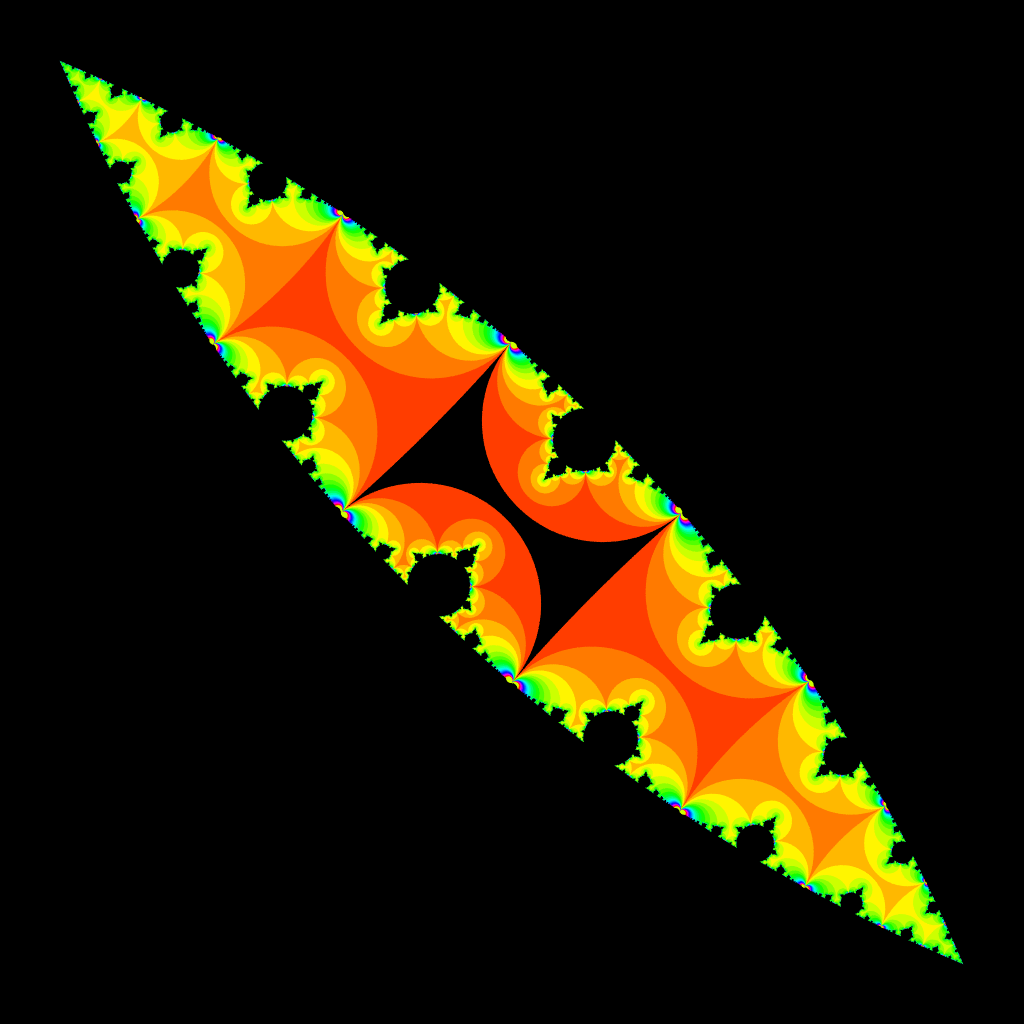
\includegraphics[height=1.35in, keepaspectratio]{img/application/internal/schottky.png}
  \subcaption{\textit{}}
  \label{fig:schottkyAll}
  \hspace*{\fill}
 \end{minipage}
 \begin{minipage}[t]{0.5\hsize}
  \center
  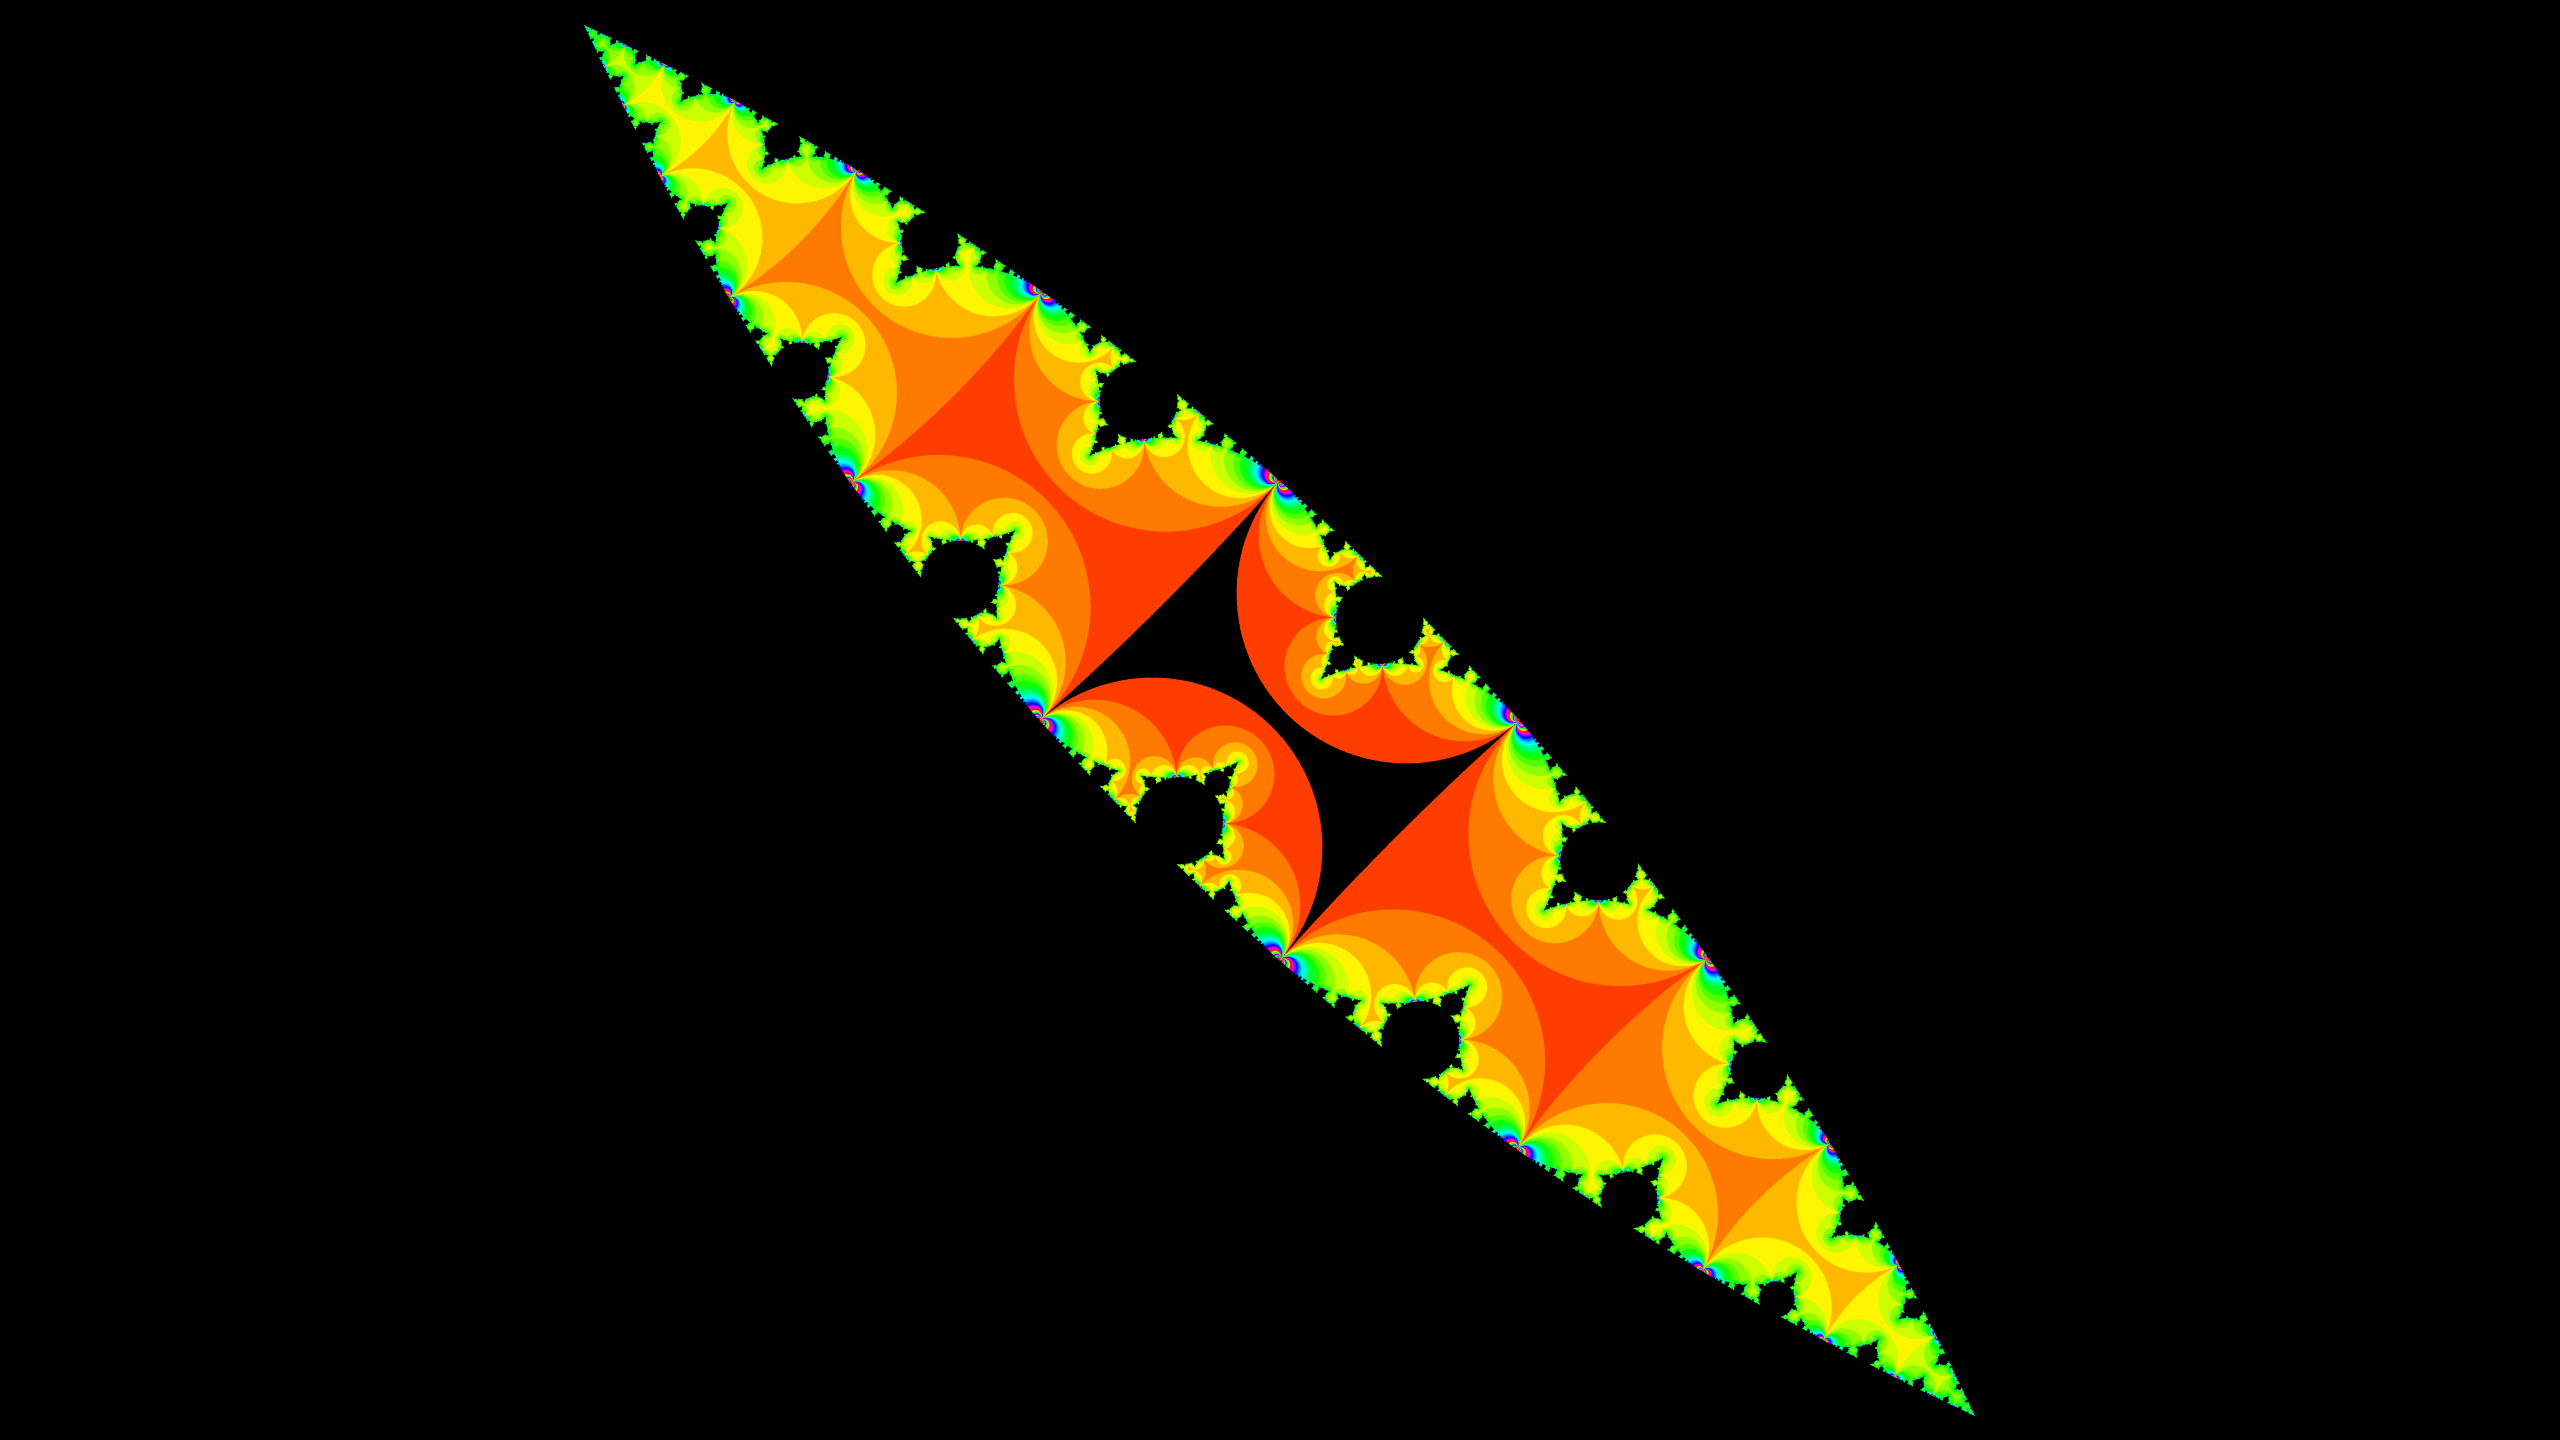
\includegraphics[height=1.35in, keepaspectratio]{img/application/internal/schottkyEdge.png}
  \subcaption{\textit{}}
  \label{fig:schottkyEdge}
  \hspace*{\fill}
 \end{minipage}
 \caption{\textit{Edge of the circle inversion fractal.}}
 \label{fig:schottkyDivide}
\end{figure}

\noindent In two-dimensional circle inversion fractals,
when all of the circles touch each other, the limit set divides the plane
into two parts as shown in Figure \ref{fig:schottkyDivide}\subref{fig:schottkyAll}.
The image generated by four inversions of circles.
After applying IIS, we only fill the pixel when the transformed point is
moved into an inner part of the black area, and we obtain the inner part
of the circle inversion fractals. See Figure
 \ref{fig:schottkyDivide}\subref{fig:schottkyEdge}.

\subsection{Render Circles}

\begin{figure}[htbp]
 \begin{minipage}[t]{0.5\hsize}
  \center
  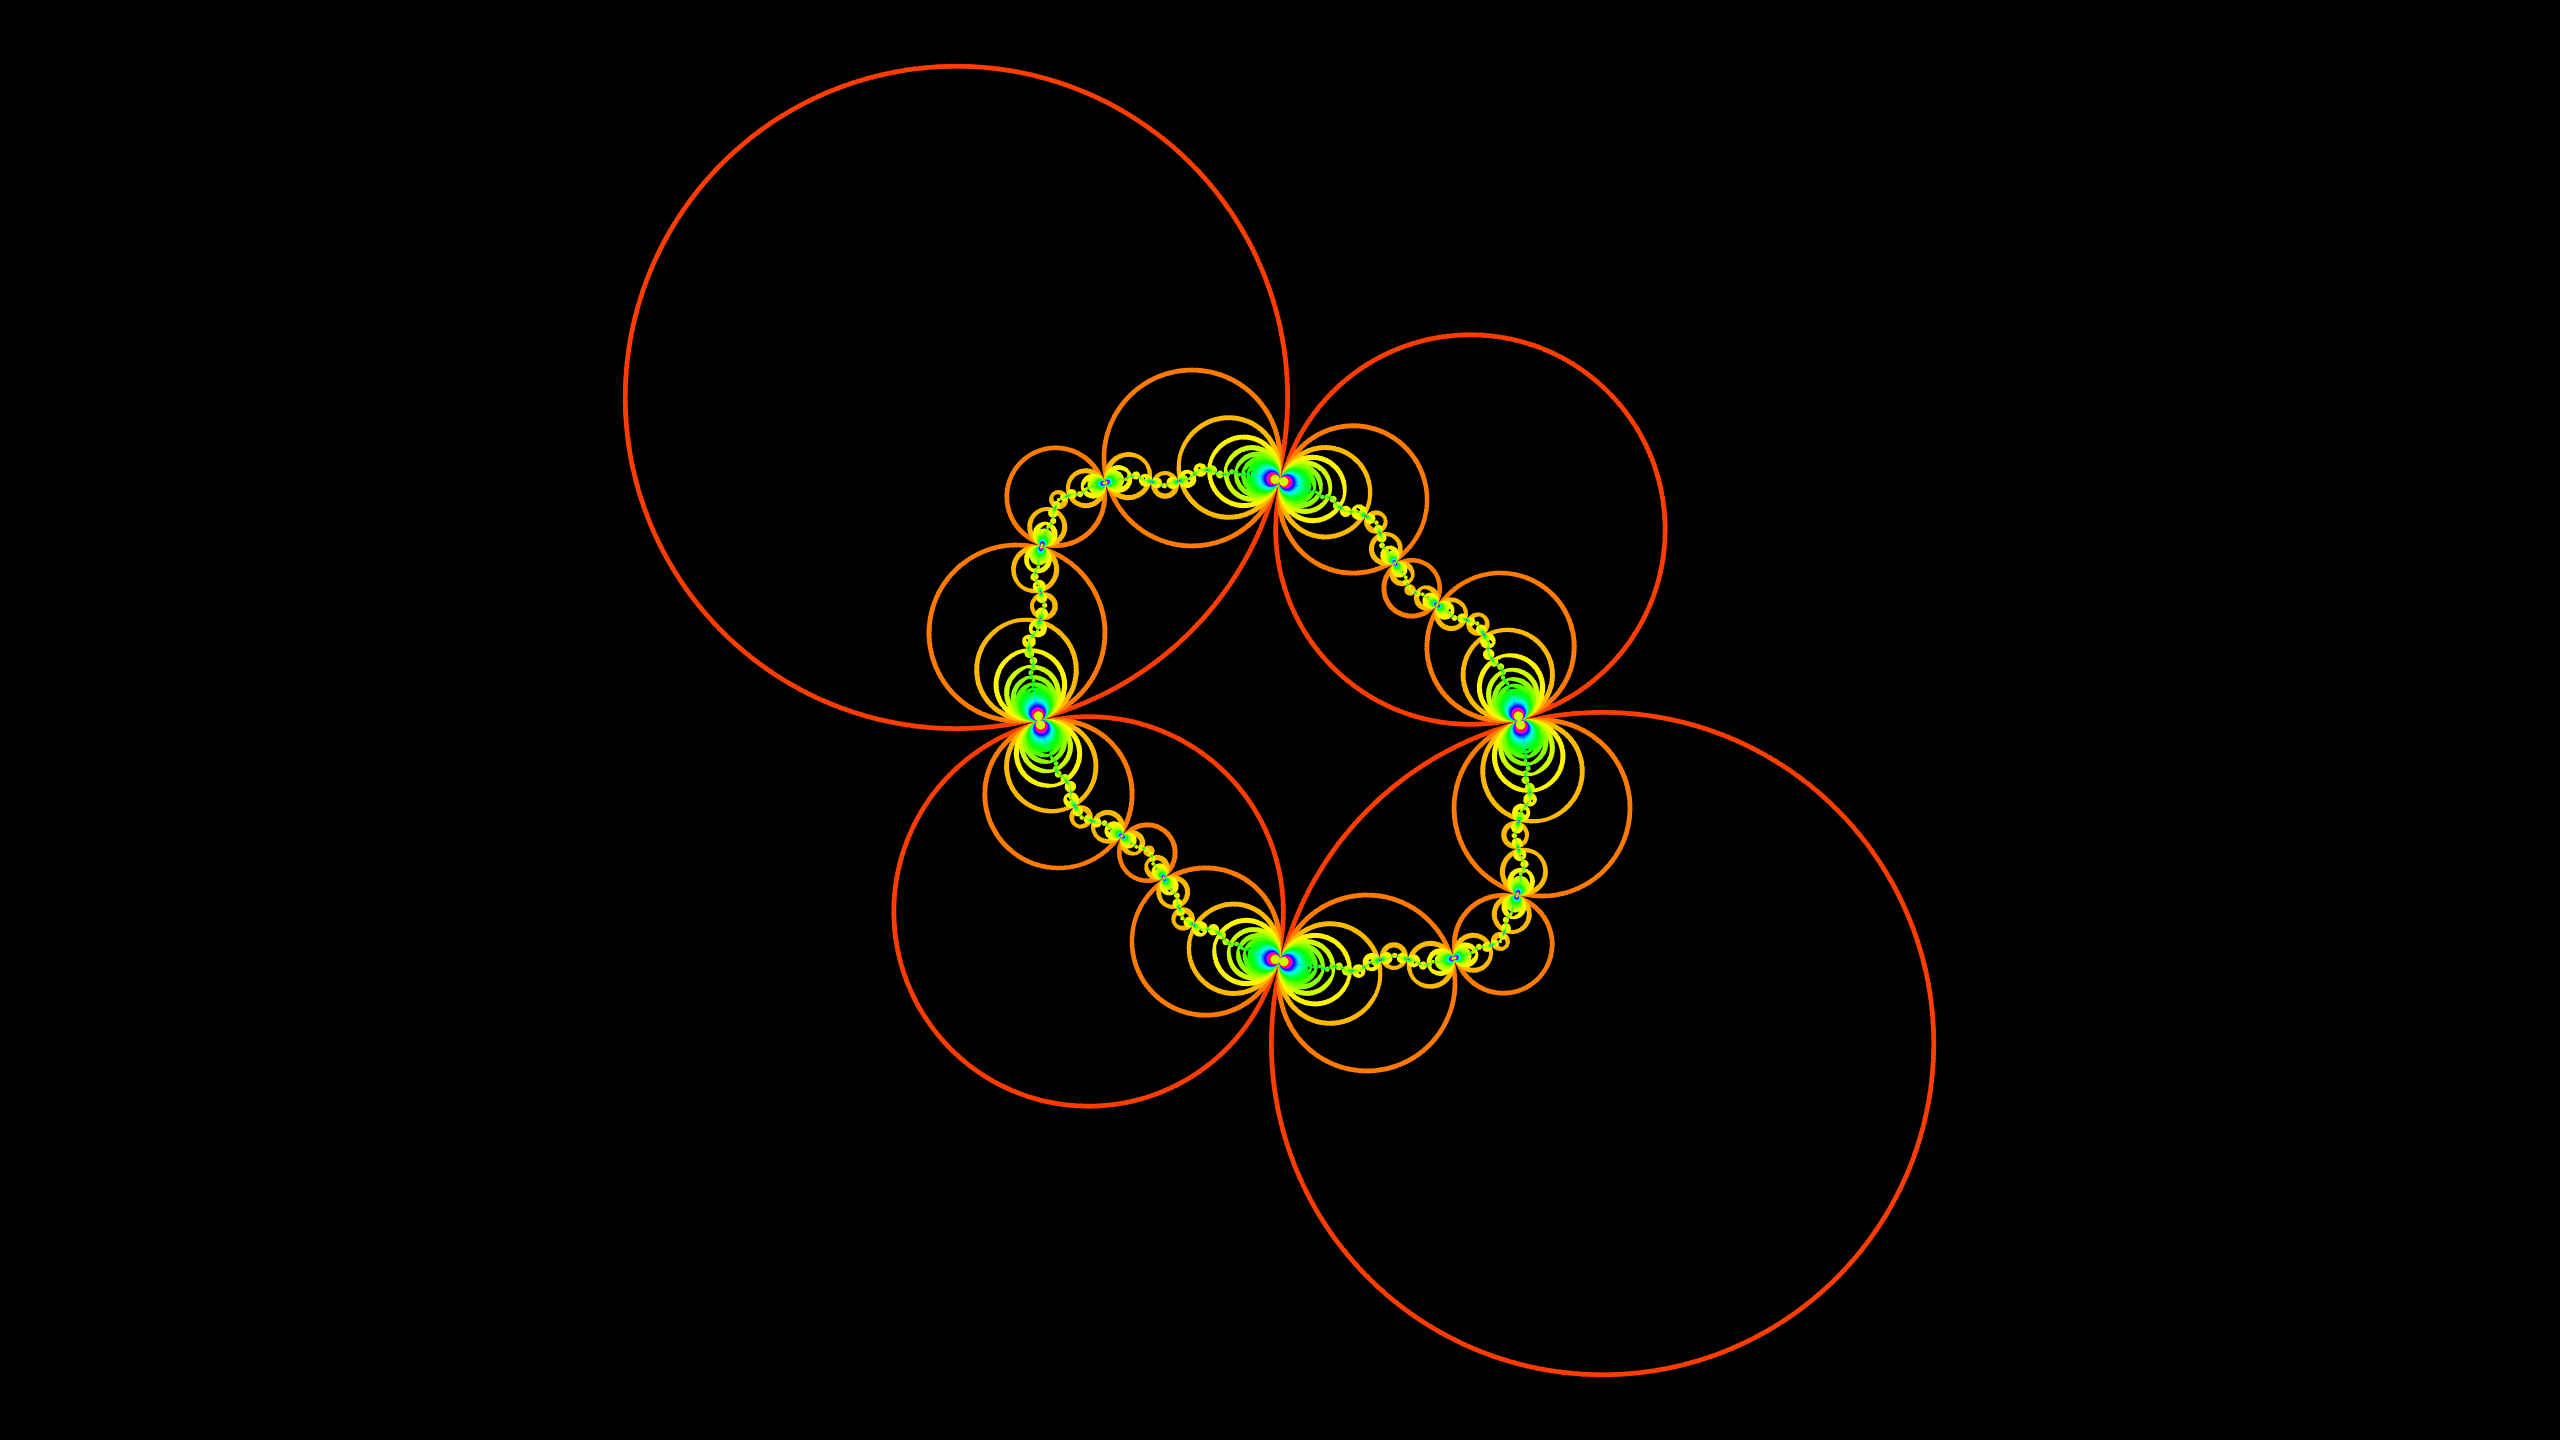
\includegraphics[height=1.35in, keepaspectratio]{img/application/edge/circles.png}
  \subcaption{\textit{}}
  \label{}
  \hspace*{\fill}
 \end{minipage}
 \begin{minipage}[t]{0.5\hsize}
  \center
  \includegraphics[height=1.35in, keepaspectratio]{img/application/edge/circleEdge.png}
  \subcaption{\textit{}}
  \label{}
  \hspace*{\fill}
 \end{minipage}
 \caption{\textit{Circle inversion fractal.}}
 \label{fig:circleEdge}
\end{figure}

\noindent
We can draw only edges of disks in circle inversion fractals as shown in
Figure \ref{fig:circleEdge}.
We can estimate the distance from the circumference of the disks using Jacobian
of circle inversions.
When we apply circle inversions, we multiply and accumulate Jacobian of
the inversions.
When the transformed point is moved to the outside of the initial disks,
we divide computed distance by accumulated Jacobian.

\subsection{Geometrical Representation of M\"obius Transformation Groups}

So far, we only use a simple circle or sphere inversions.
Other interesting images can be generated using more
complicated M\"obius transformations.
It is known that we can construct any M\"obius transformation out of
inversions. We can compose them by an even number of inversion.
Thus, we can apply IIS to visualize fractals combining circle inversion
fractals and extended M\"obius transformation groups.
Moreover, we can tweak the parameters of M\"obius transformations by
arranging geometrical objects like circles or lines on the plane.
So, we can control parameters easily and intuitively.

The author is developing visualization software for inversion fractals.
It is available at \url{https://schottky.jp}.
This section is a revised version of \cite{bridges2017:159}.

\subsubsection{Two Dimensionanl Generators}

\begin{figure}[htbp]
 \begin{minipage}[t]{0.5\hsize}
  \begin{minipage}{0.25\hsize}
   \center
   
\includegraphics[ height=1.4in, keepaspectratio]{./img/application/2dGen/infInvEdgedGen.pdf}
   \subcaption{\textit{Generator}}
   \label{fig:infCircleGen}
  \end{minipage}
  \hspace*{\fill}
  \begin{minipage}{0.25\hsize}
   \center
   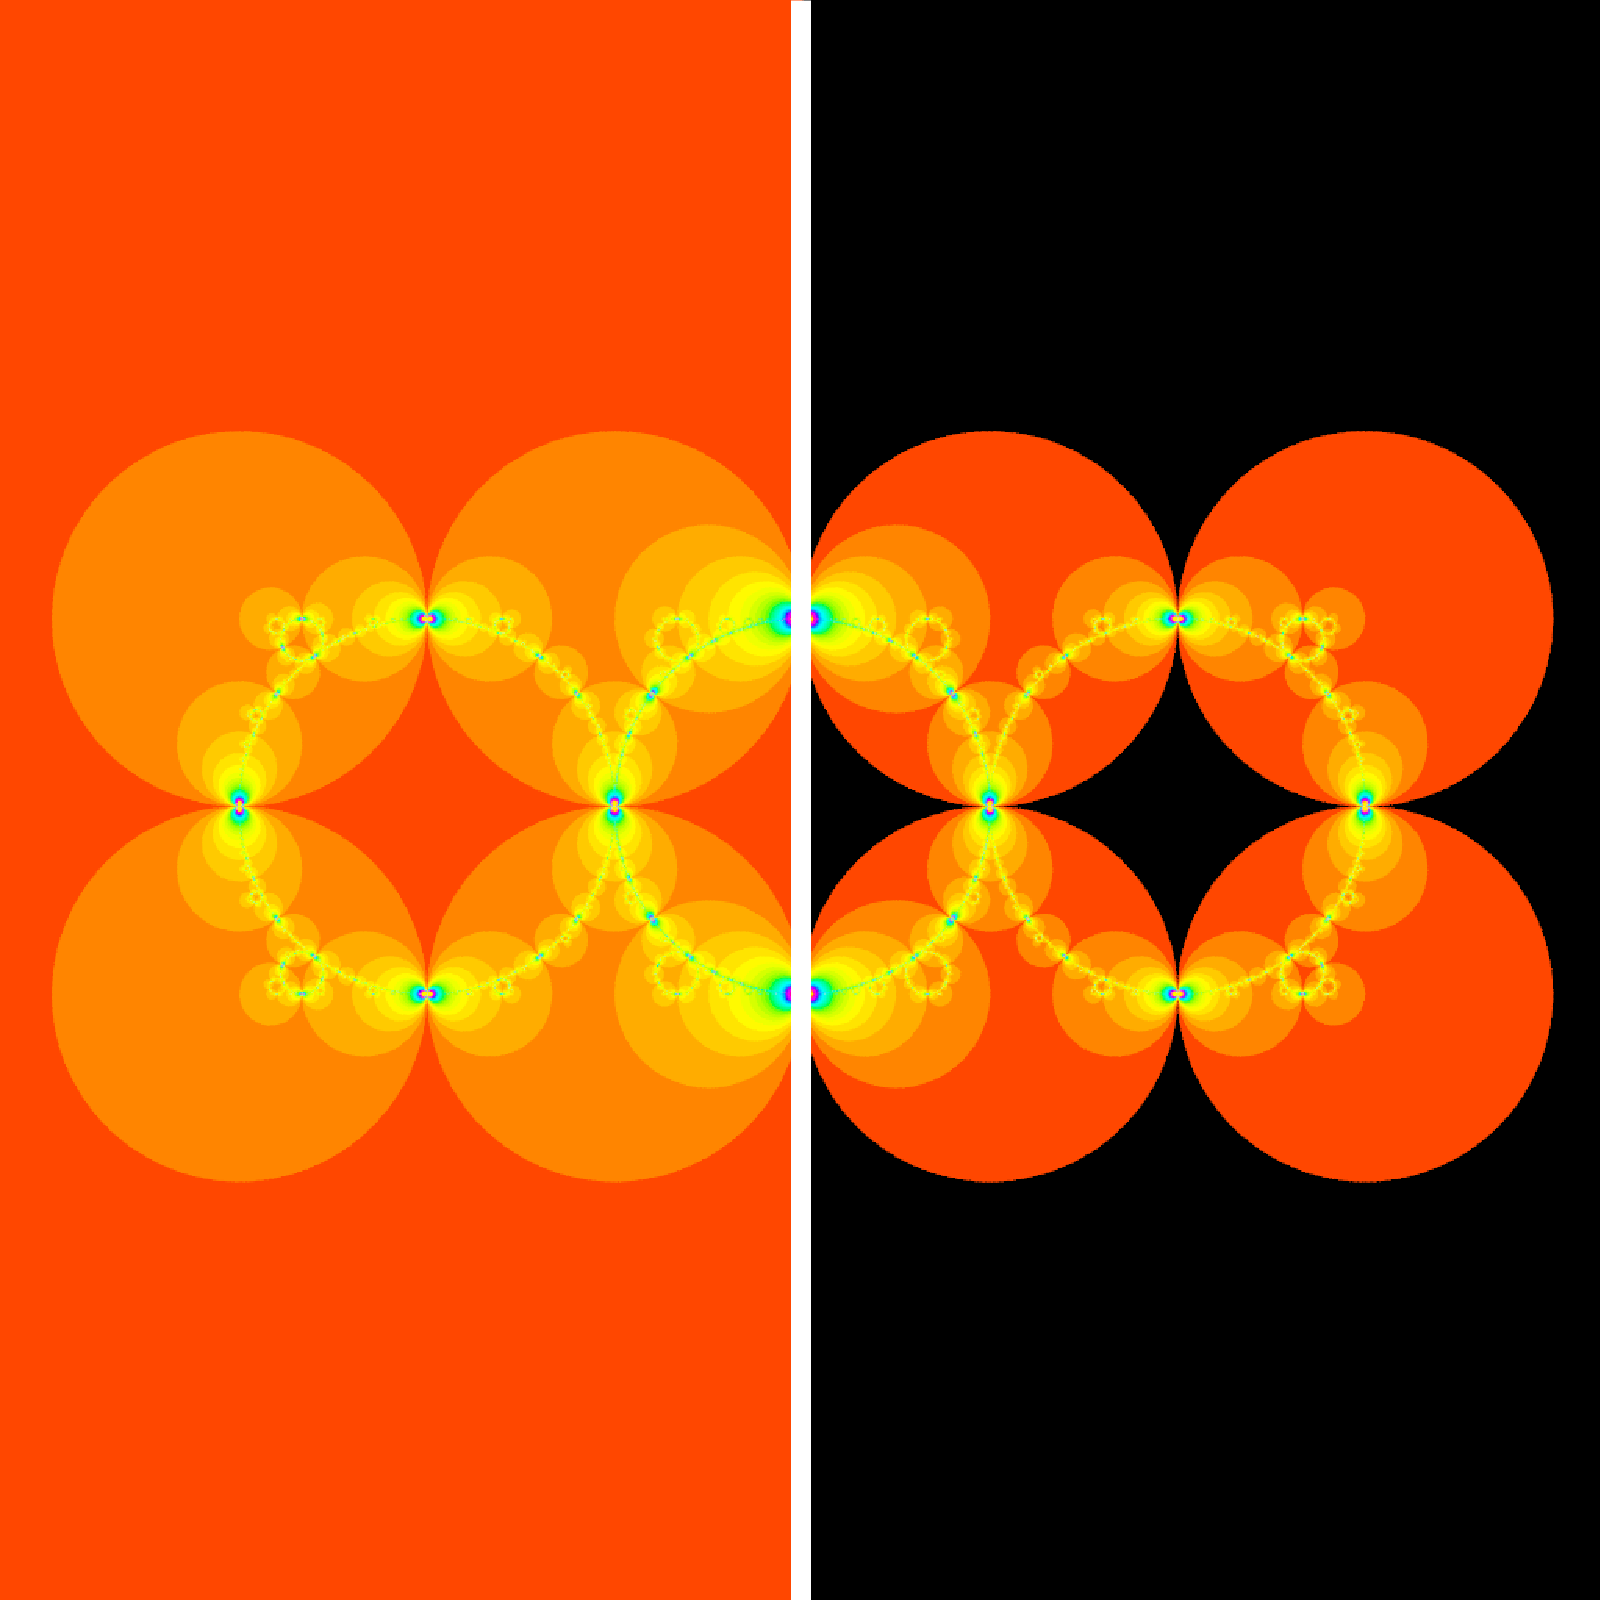
\includegraphics[ height=1.4in, keepaspectratio]{./img/application/2dGen/infInvEdgedOrb.pdf}
   \subcaption{\textit{Orbit}}
   \label{fig:infCircleOrb}
  \end{minipage}
  \hspace*{\fill}
  \caption{\textit{Inversion in the circle with \\ infinite radius and
  four Schottky disks.}}
  \label{fig:infCircle}
 \end{minipage}
 \begin{minipage}[t]{0.5\hsize}
  \begin{minipage}{0.25\hsize}
   \center
   
\includegraphics[ height=1.4in, keepaspectratio]{./img/application/2dGen/translationEdgedGen.pdf}
   \subcaption{\textit{Generator}}
   \label{fig:translation2dGen}
  \end{minipage}
  \hspace*{\fill}
  \begin{minipage}{0.25\hsize}
   \center
   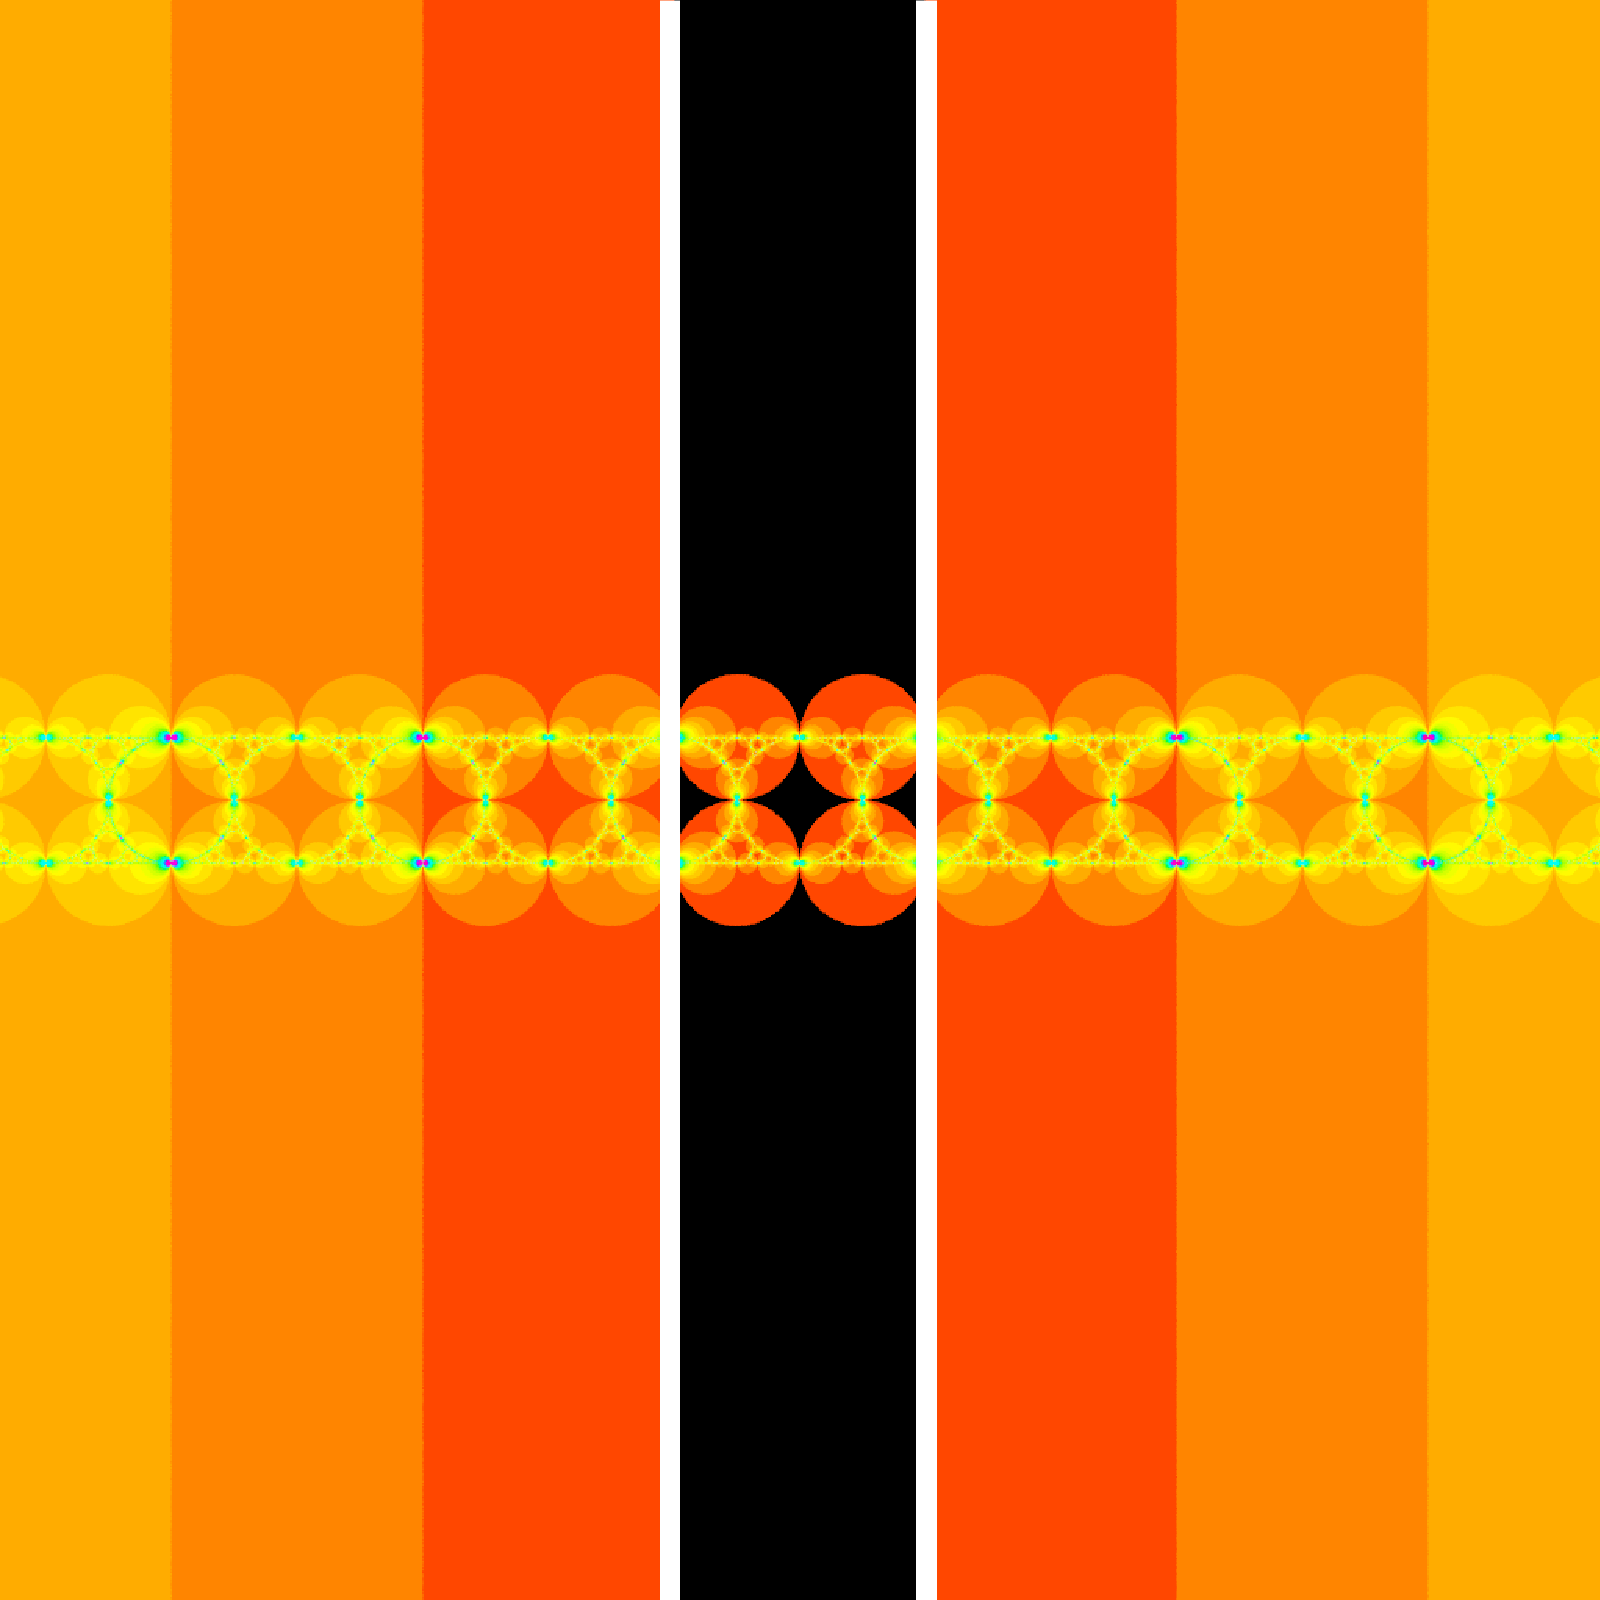
\includegraphics[ height=1.4in, keepaspectratio]{./img/application/2dGen/translationEdgedOrb.pdf}
   \subcaption{\textit{Orbit}}
   \label{fig:translation2dOrb}
  \end{minipage}
  \hspace*{\fill}
  \caption{\textit{Parallel translation generator and four Schottky disks.}}
  \label{fig:translation2d}
 \end{minipage}
 \end{figure}

\begin{figure}[htbp]
 \begin{minipage}{0.5\hsize}
  \begin{minipage}{0.25\hsize}
   \center
   
\includegraphics[ height=1.4in, keepaspectratio]{./img/application/2dGen/rotationEdgedGen.pdf}
   \subcaption{\textit{Generator}}
   \label{fig:rotation2dGen}
  \end{minipage}
 \hspace*{\fill}
  \begin{minipage}{0.25\hsize}
   \center
   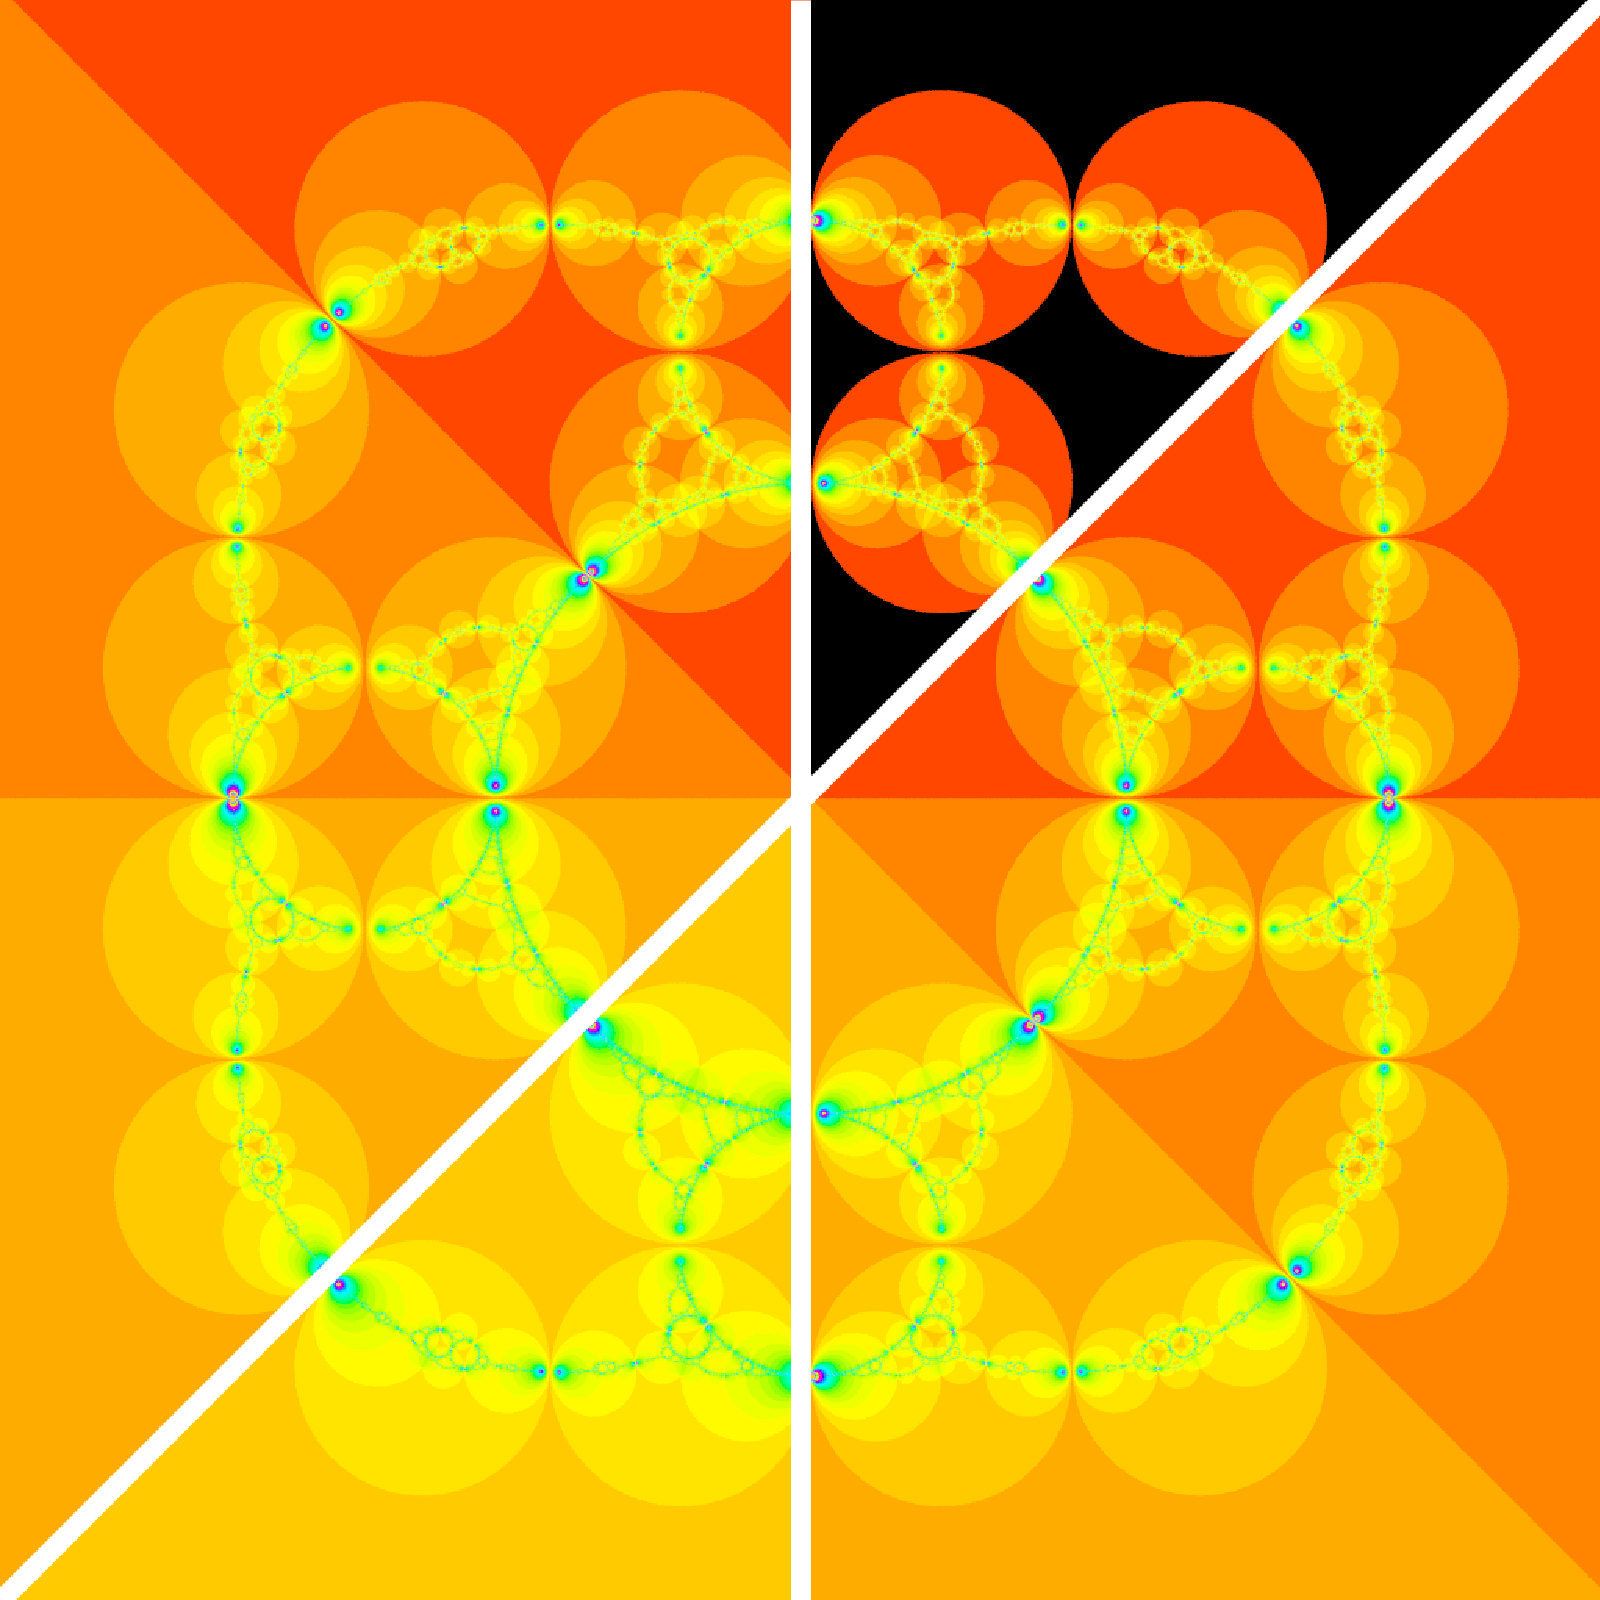
\includegraphics[ height=1.4in, keepaspectratio]{./img/application/2dGen/rotationEdgedOrb.pdf}
   \subcaption{\textit{Orbit}}
   \label{fig:rotation2dOrb}
  \end{minipage}
  \hspace*{\fill}
  \caption{\textit{Rotation generator and three Schottky disks.}}
  \label{fig:rotation2d}
 \end{minipage}
 \begin{minipage}{0.5\hsize}
  \begin{minipage}{0.25\hsize}
   \center
   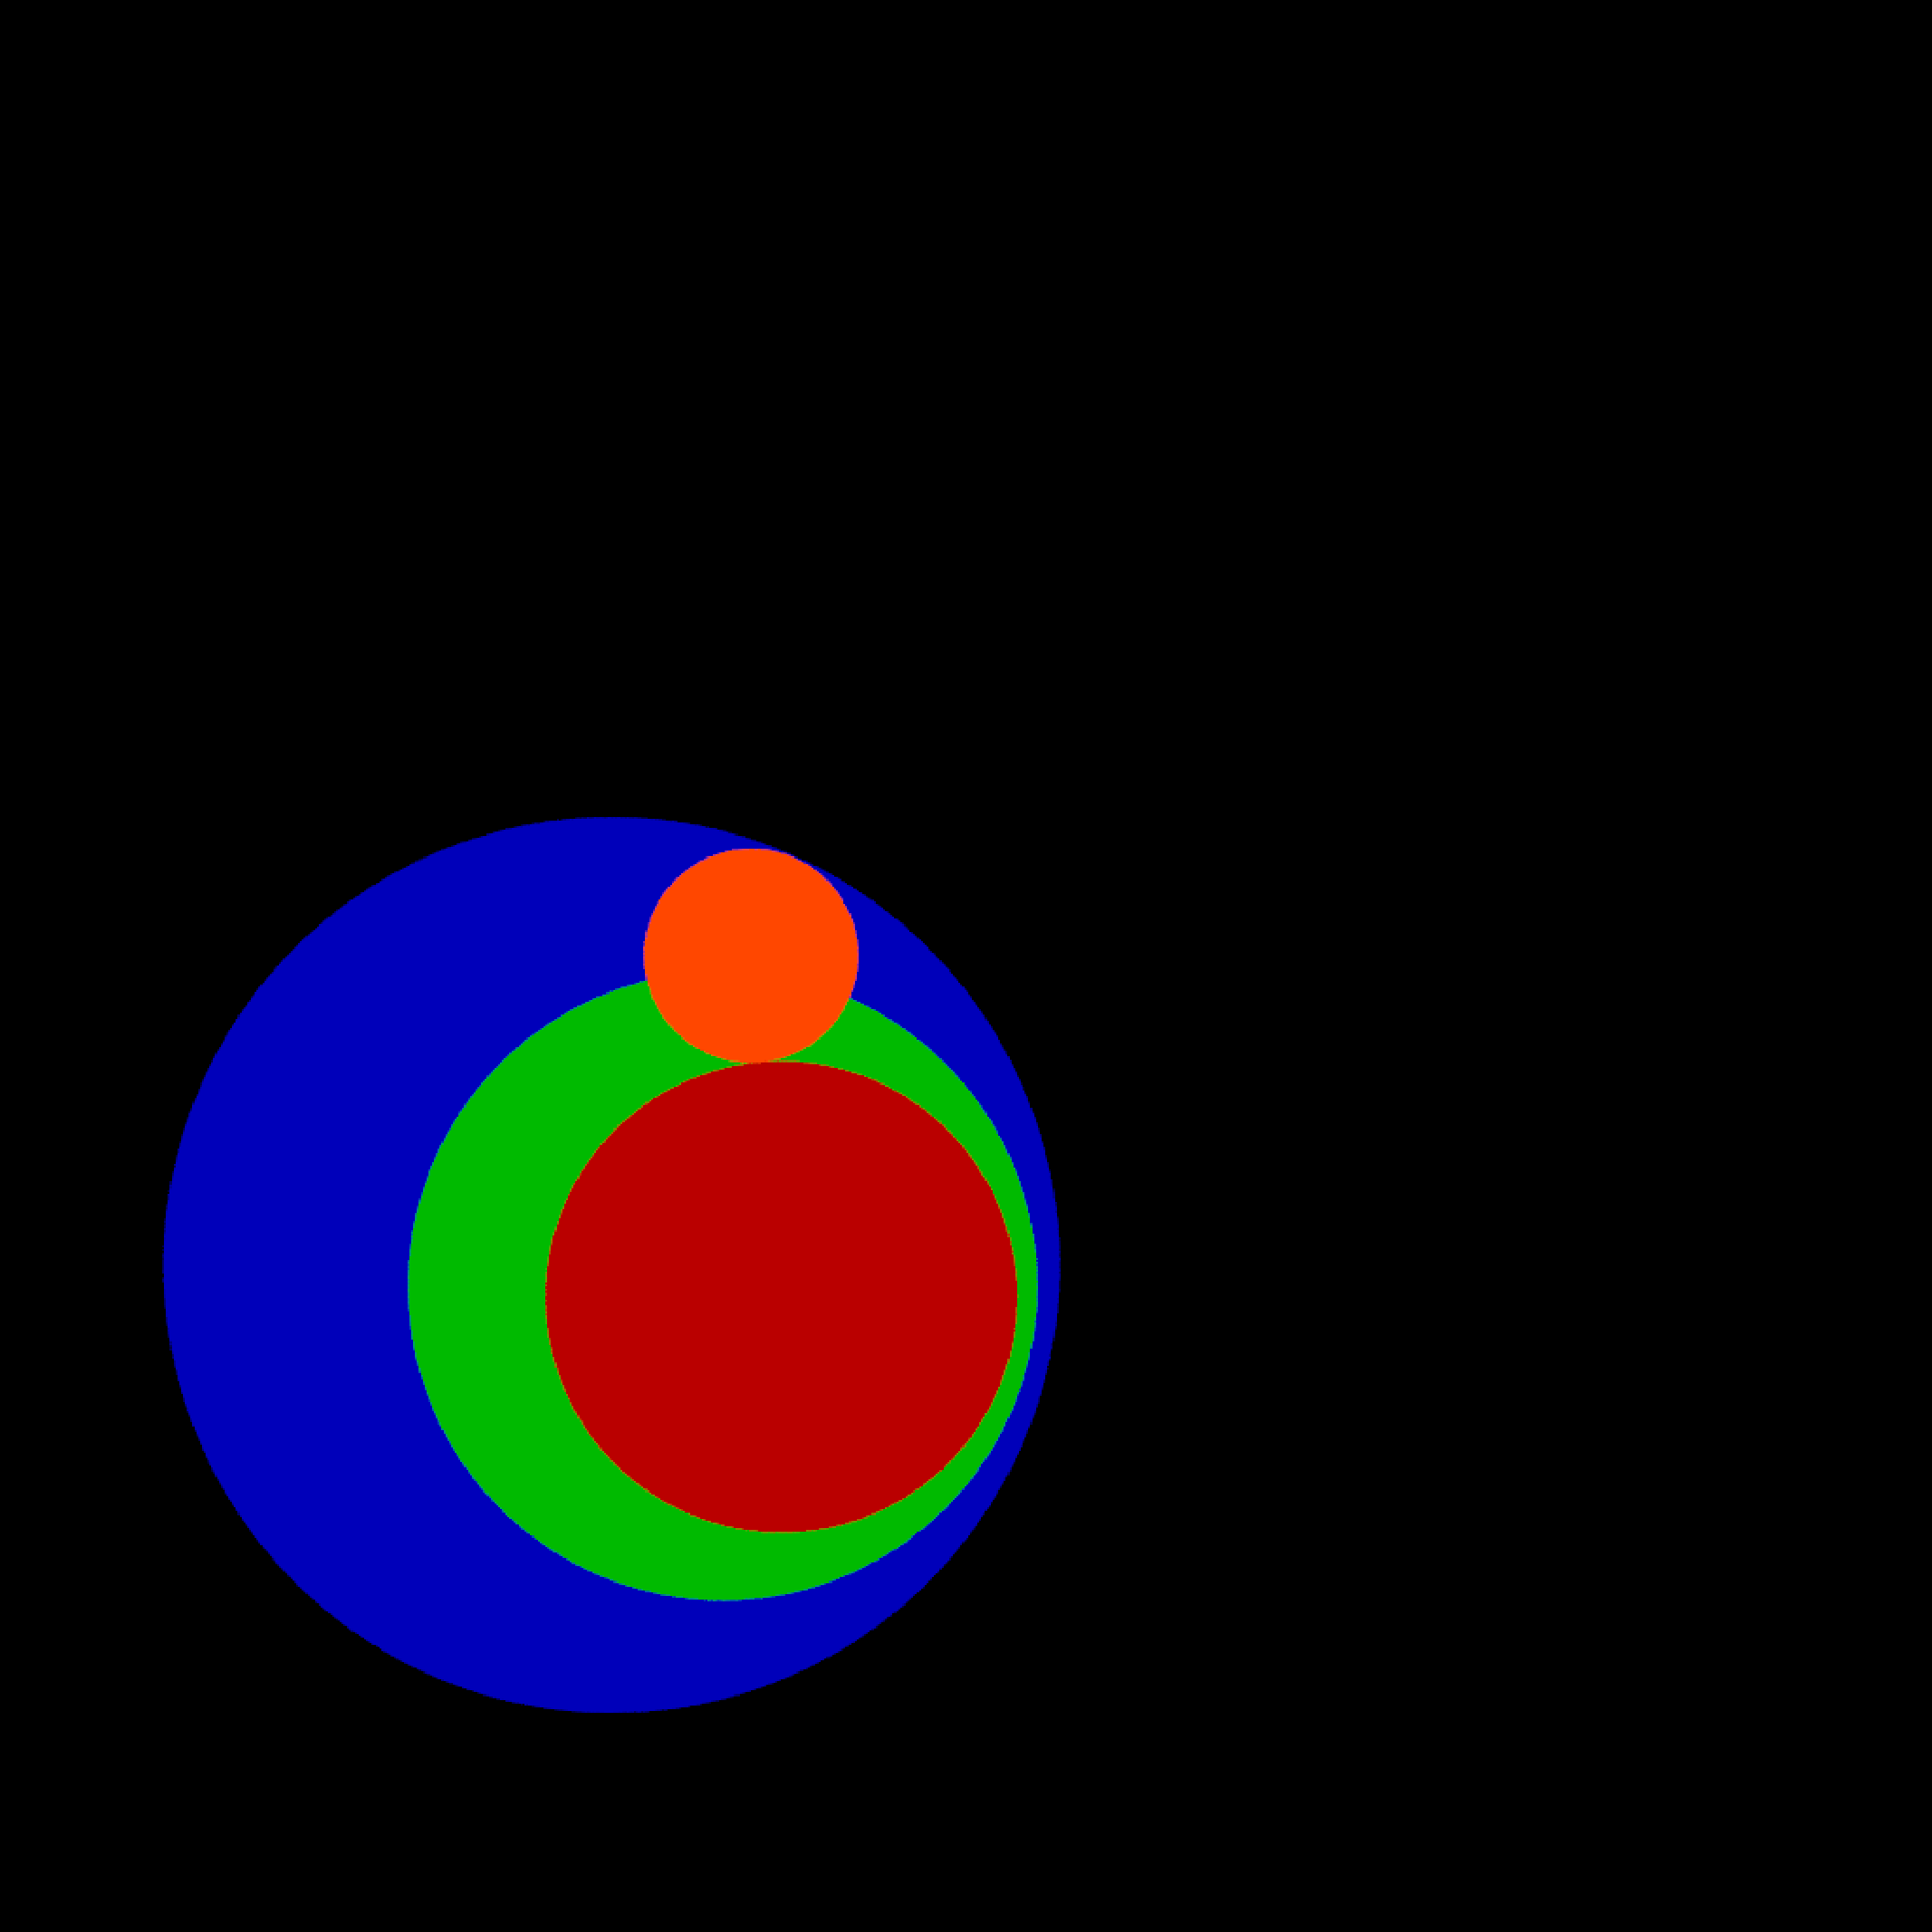
\includegraphics[ height=1.4in, keepaspectratio]{./img/application/2dGen/hyperbolicRect0.pdf}
   \subcaption{\textit{Generator}}
   \label{fig:hyperbolic2dGen}
  \end{minipage}
 \hspace*{\fill}
  \begin{minipage}{0.25\hsize}
   \center
   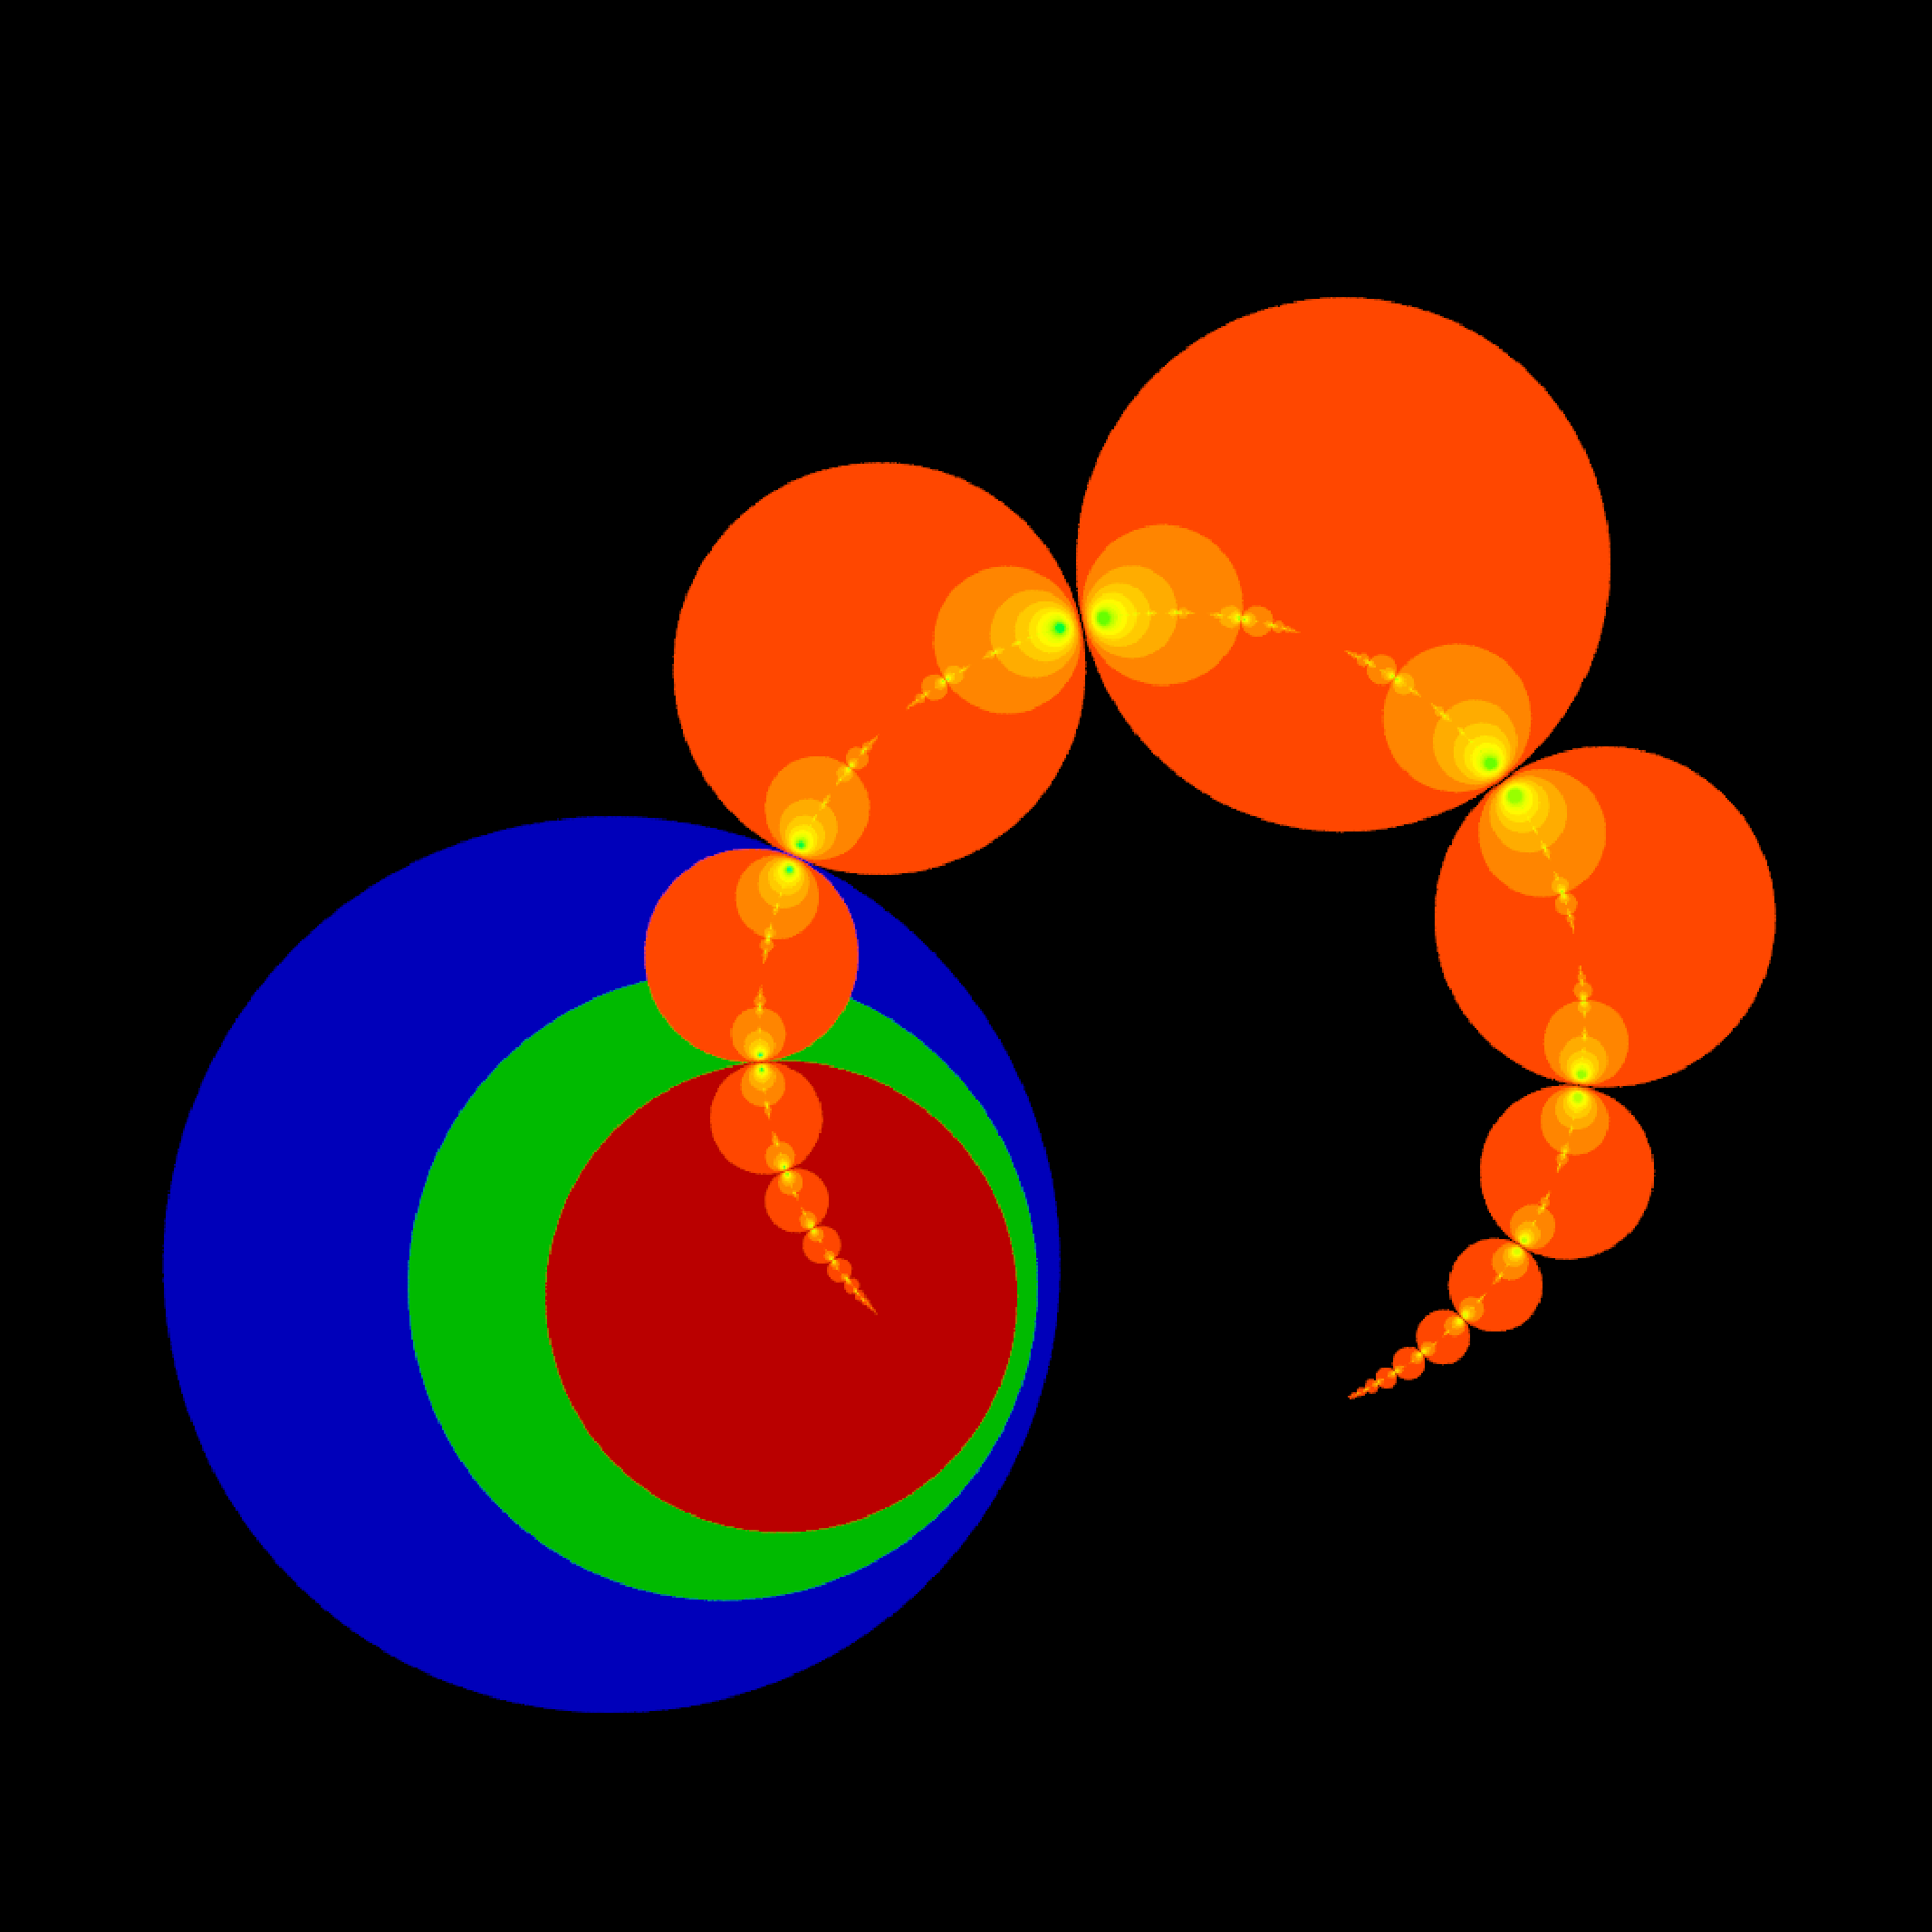
\includegraphics[ height=1.4in, keepaspectratio]{./img/application/2dGen/hyperbolicRect.pdf}
   \subcaption{\textit{Orbit}}
   \label{fig:hyperbolic2dOrb}
  \end{minipage}
 \hspace*{\fill}
  \caption{\textit{Hyperbolic generator and a Schottky disk.}}
  \label{fig:hyperbolic2d}
 \end{minipage}
\end{figure}

\begin{figure}[htbp]
 \begin{minipage}[t]{0.5\hsize}
  \begin{minipage}{0.25\hsize}
   \center
   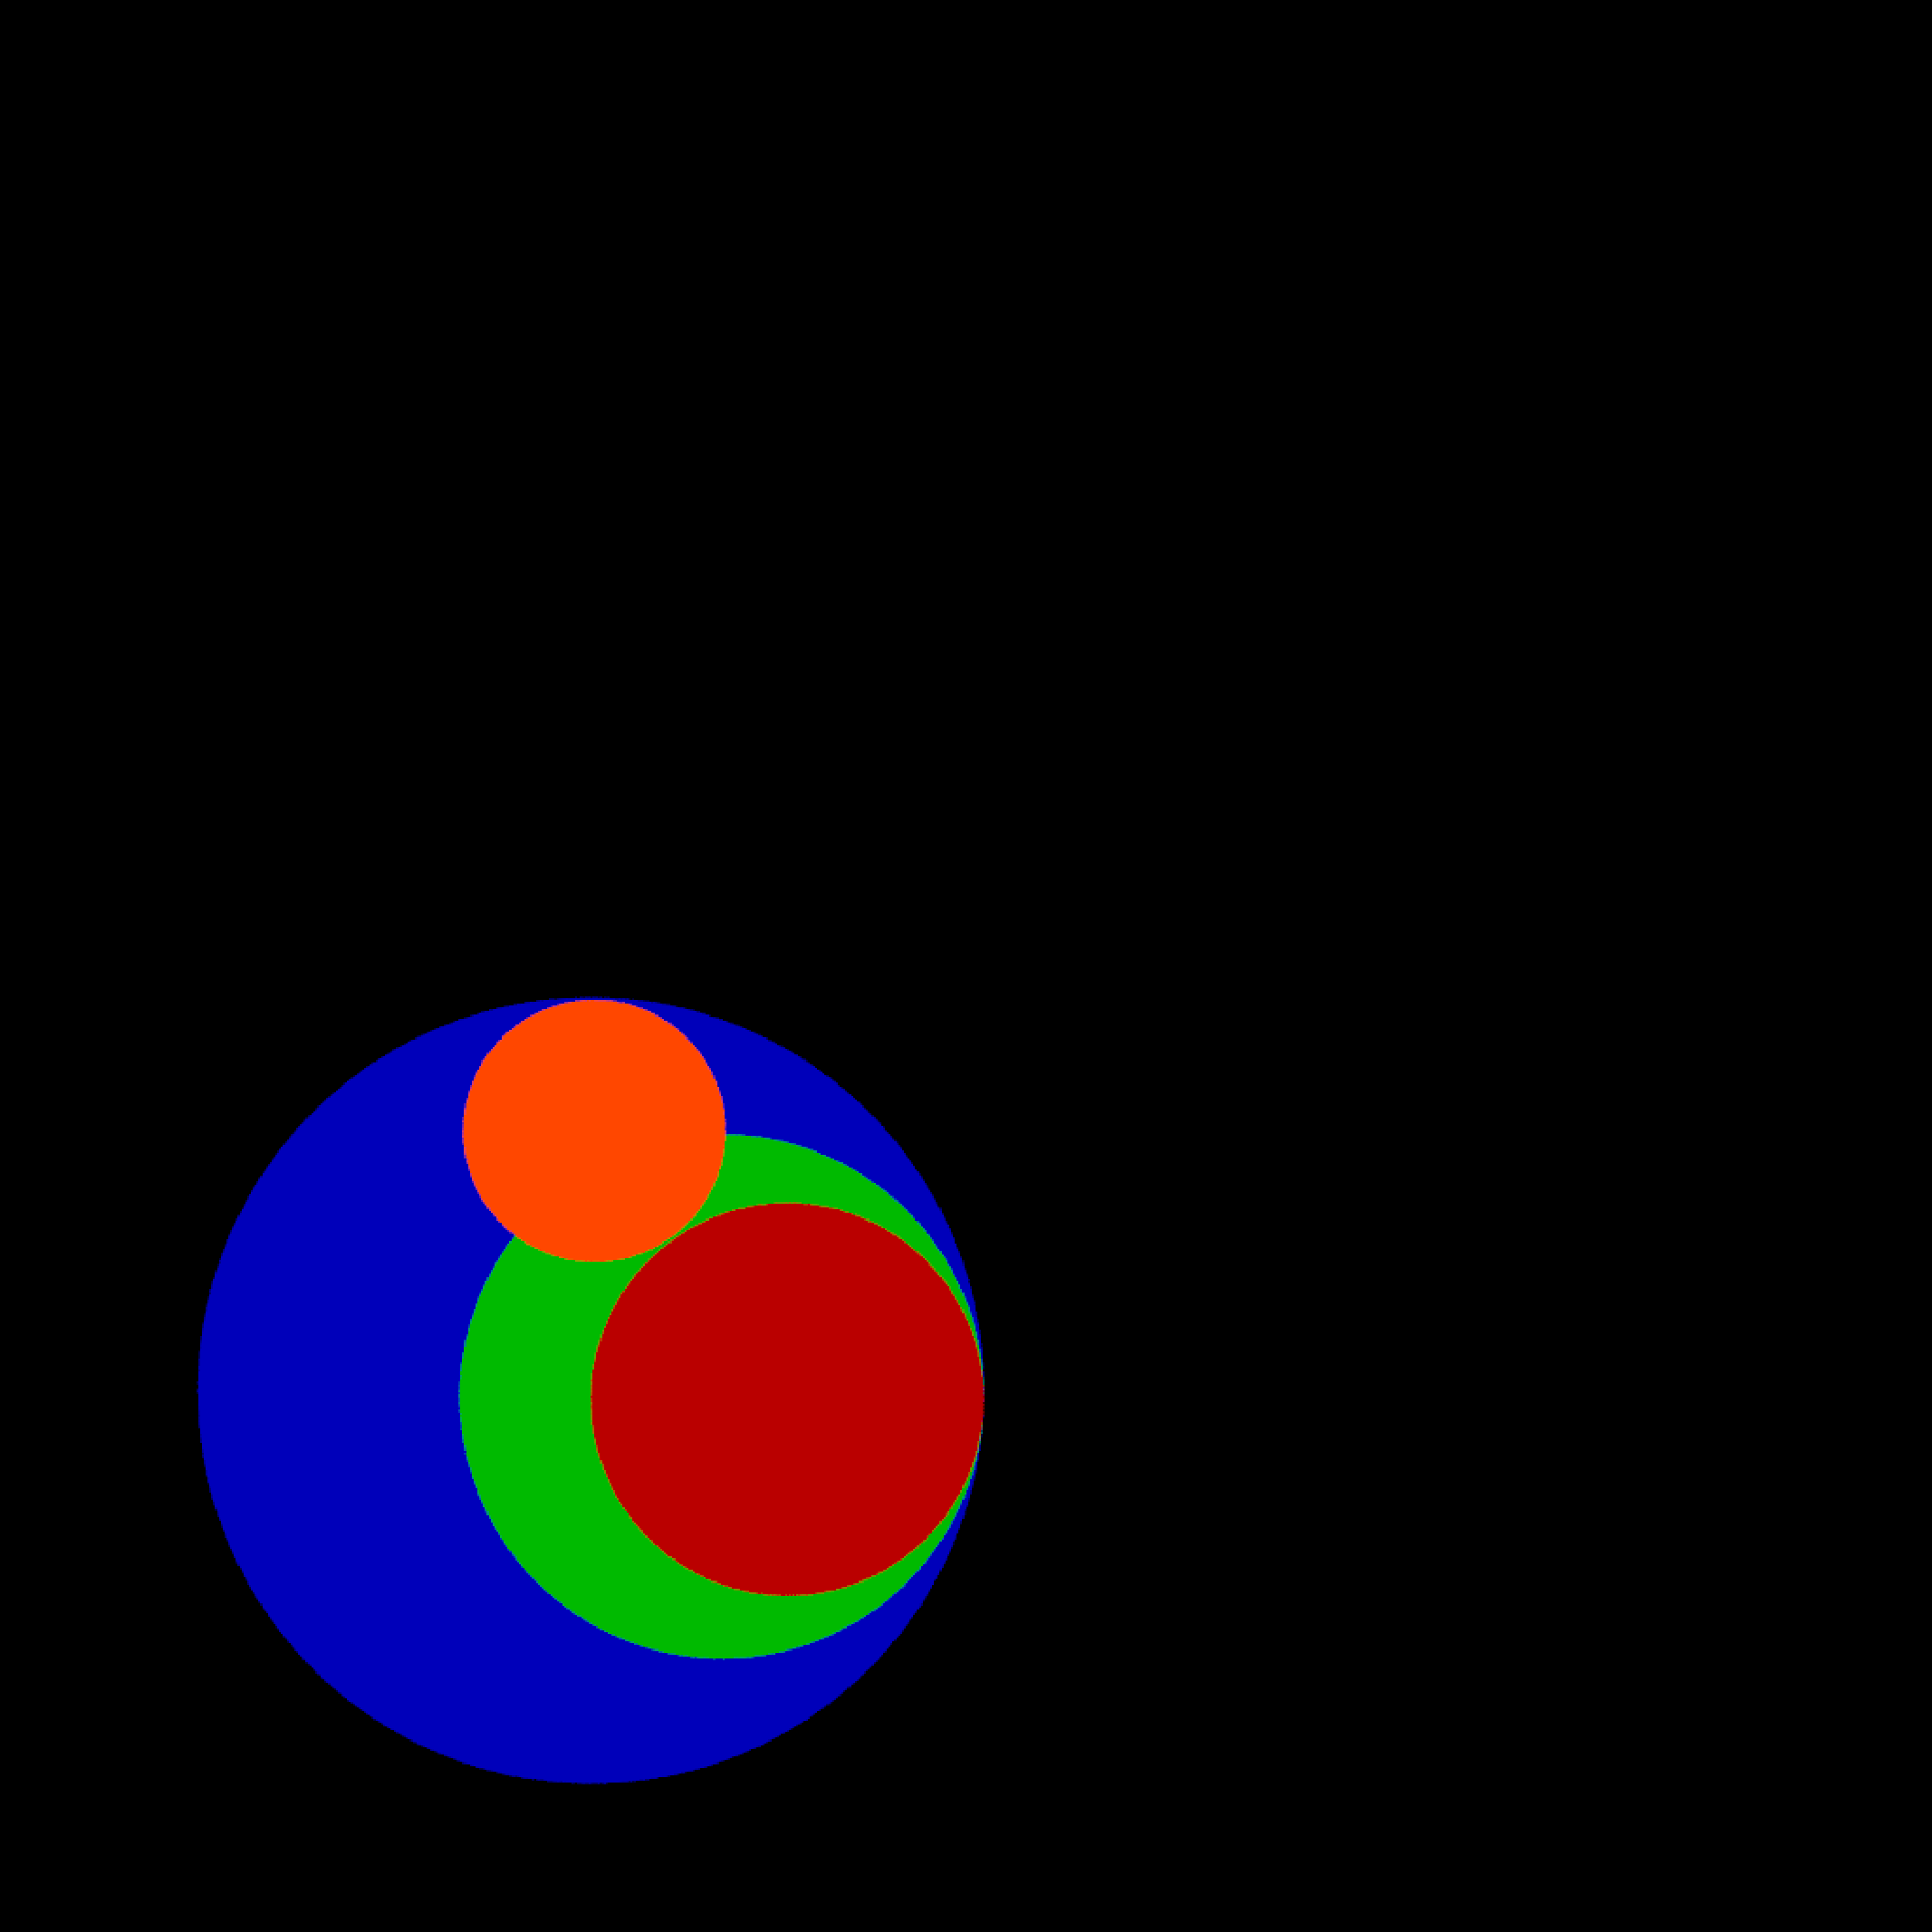
\includegraphics[ height=1.4in, keepaspectratio]{./img/application/2dGen/parabolicRect0.pdf}
   \subcaption{\textit{Generator}}
   \label{fig:parabolic2dGen}
  \end{minipage}
 \hspace*{\fill}
  \begin{minipage}{0.25\hsize}
   \center
   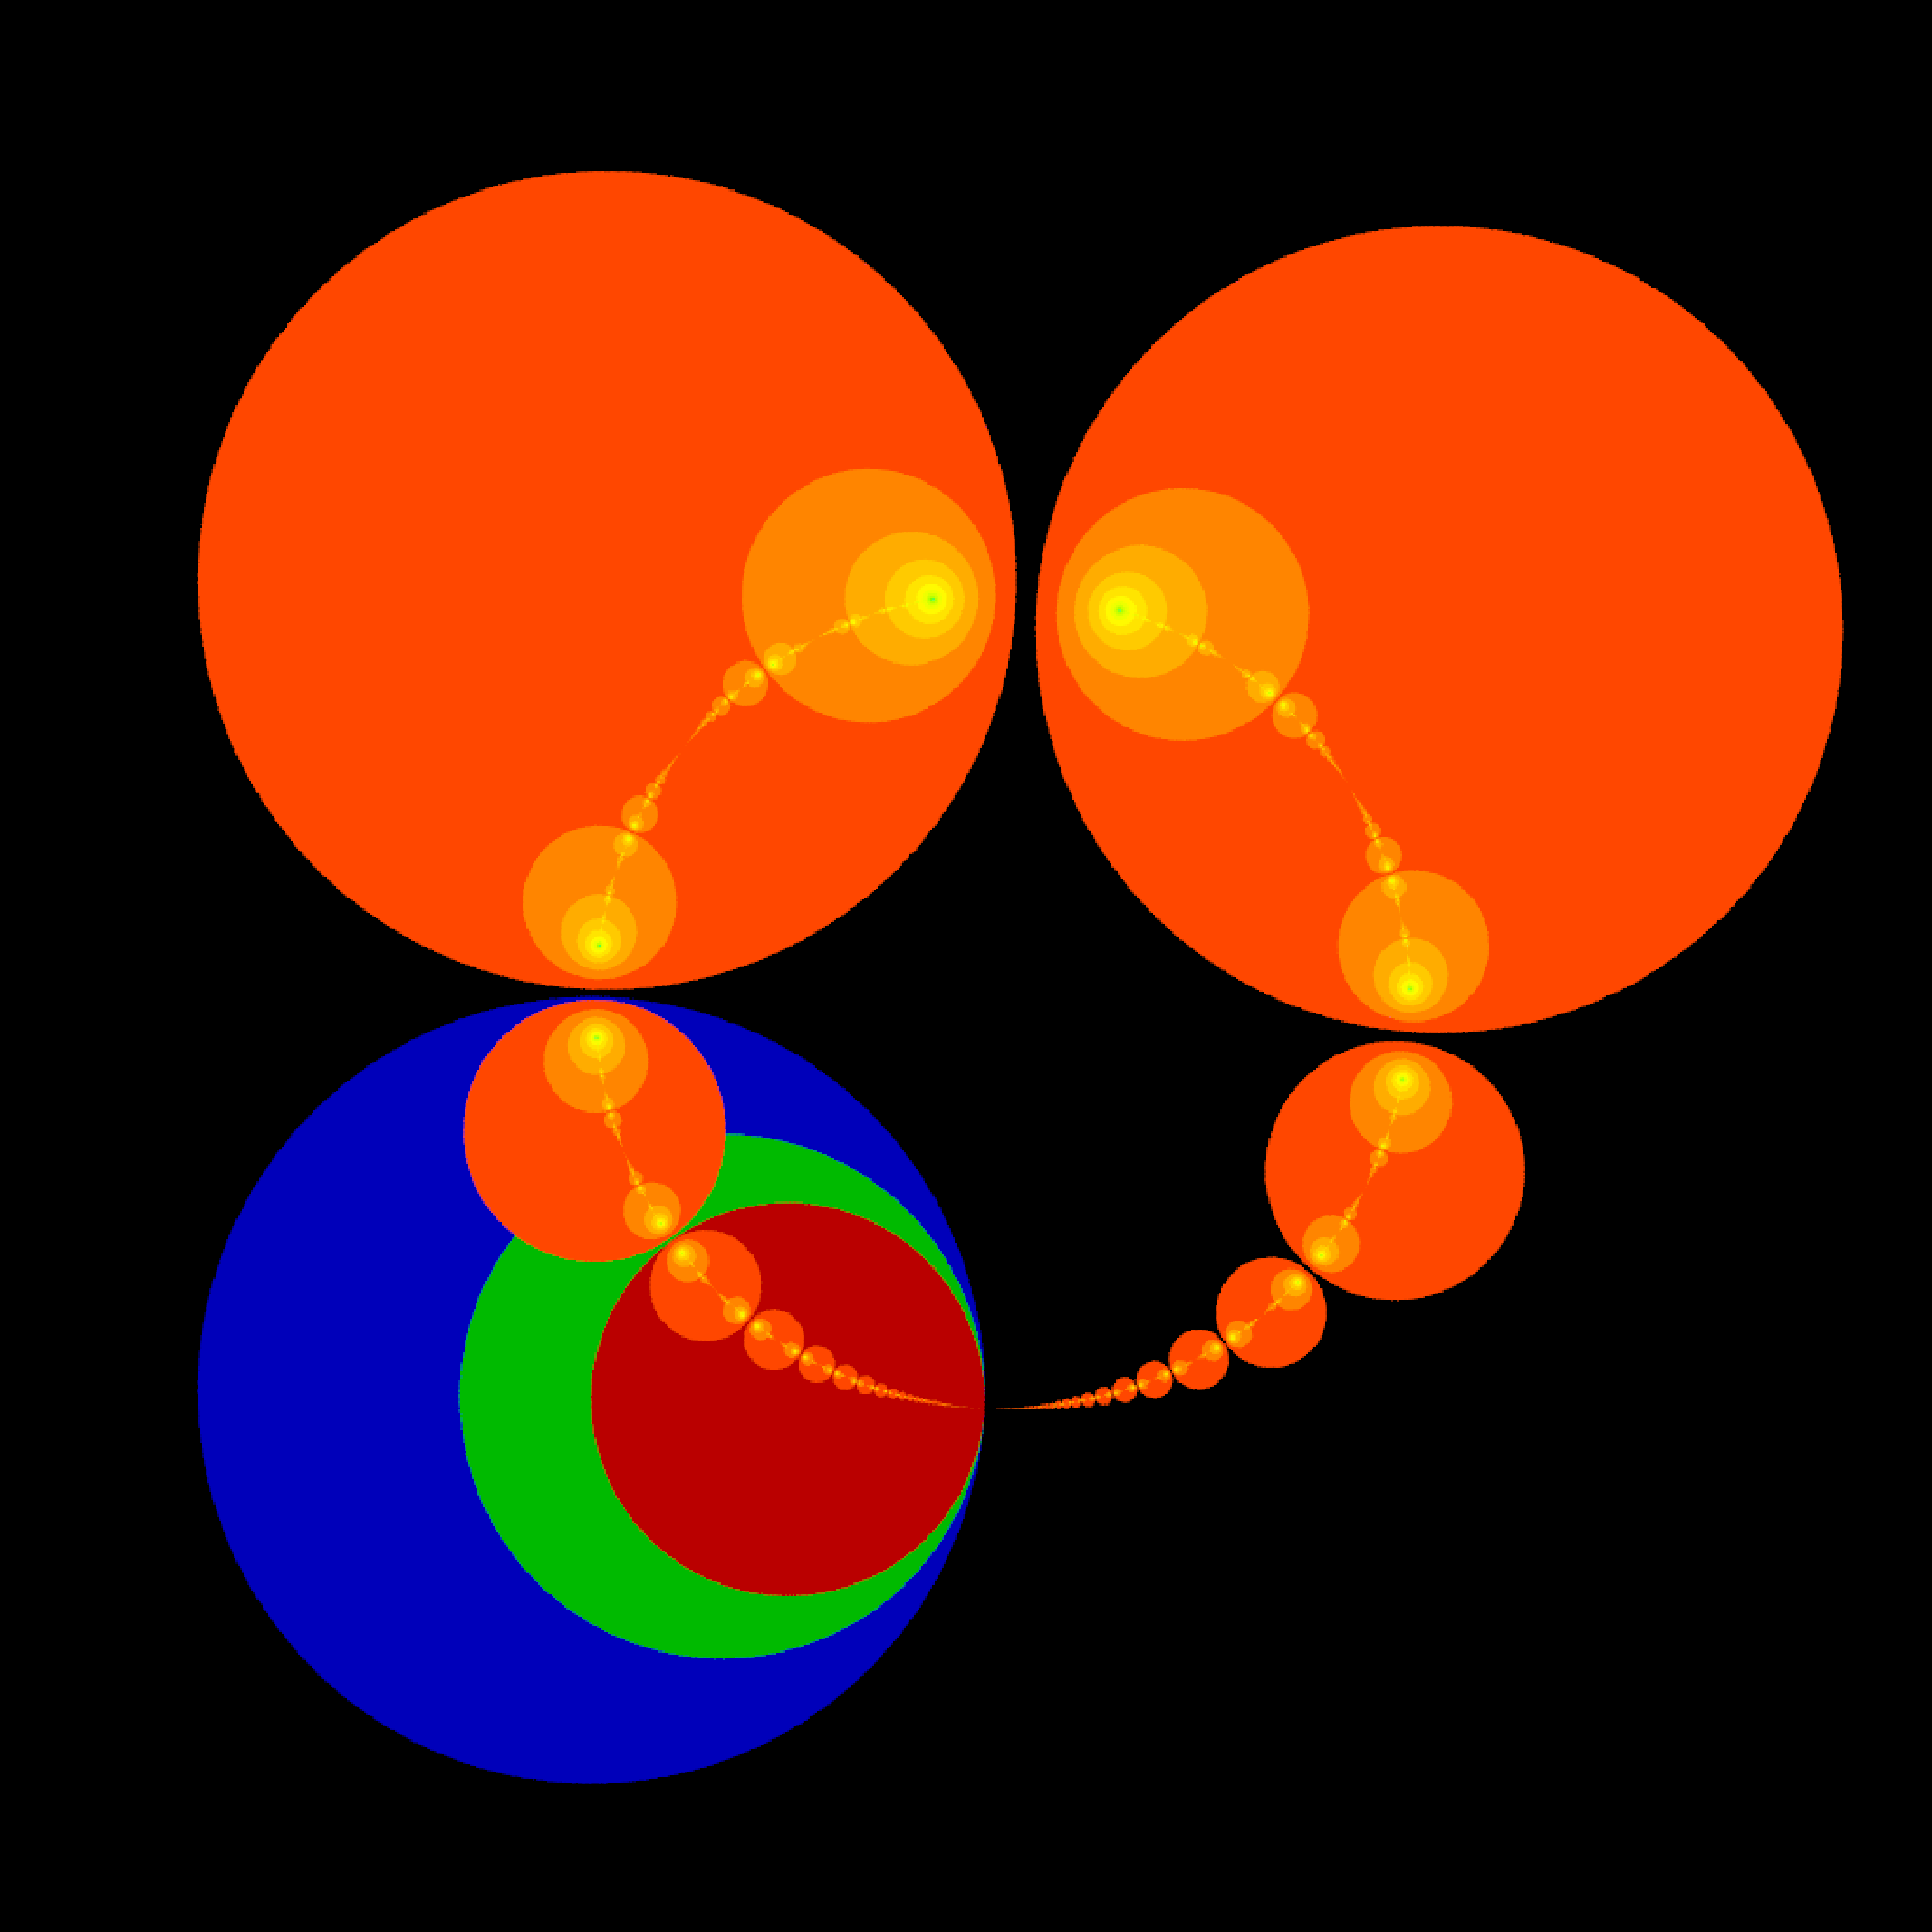
\includegraphics[ height=1.4in, keepaspectratio]{./img/application/2dGen/parabolicRect.pdf}
   \subcaption{\textit{Orbit}}
   \label{fig:parabolic2dOrb}
  \end{minipage}
  \hspace*{\fill}
  \caption{\textit{The orbit of Parabolic generator and \\a Schottky disk.}}
  \label{fig:parabolic2d}
 \end{minipage}
 \begin{minipage}[t]{0.5\hsize}
  \begin{minipage}{0.25\hsize}
   \center
   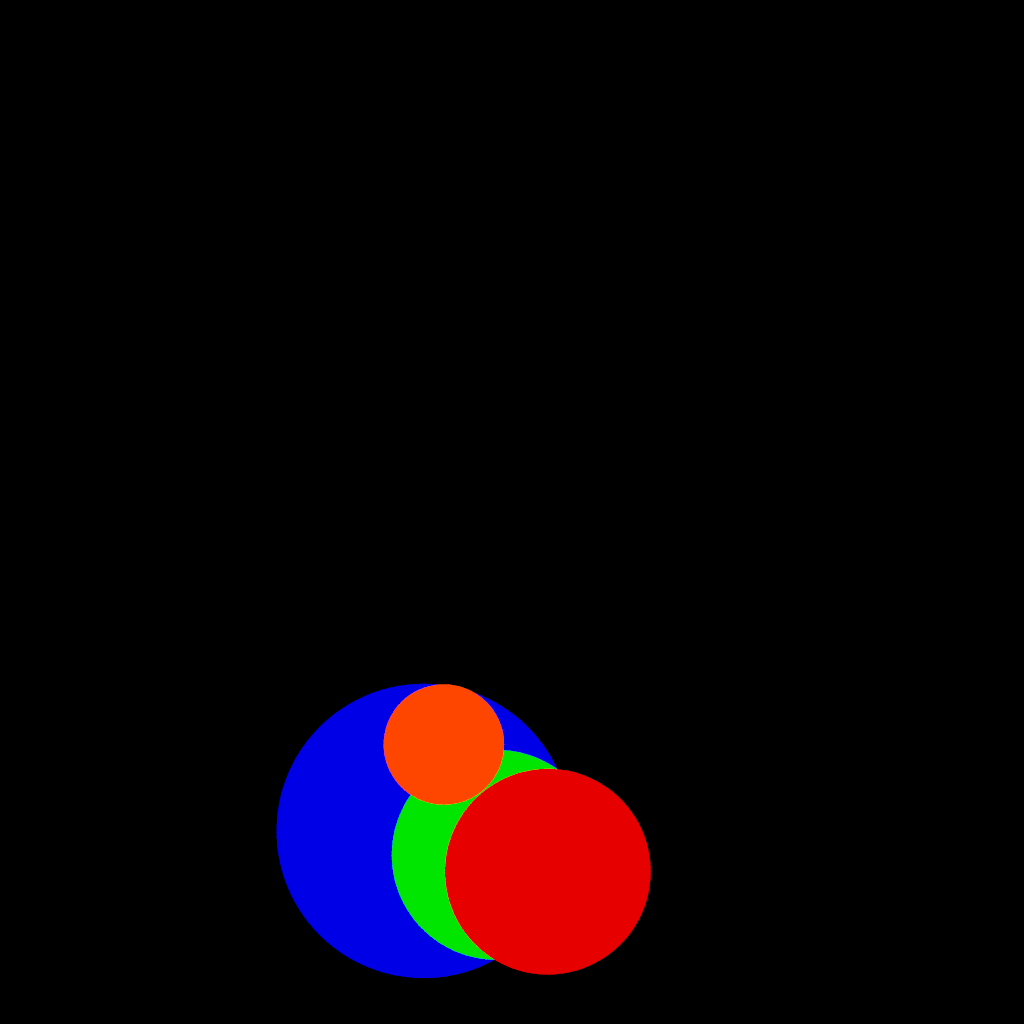
\includegraphics[ height=1.4in, keepaspectratio]{./img/application/2dGen/ellipticGen.png}
   \subcaption{\textit{Generator}}
   \label{fig:elliptic2dGen}
  \end{minipage}
 \hspace*{\fill}
  \begin{minipage}{0.25\hsize}
   \center
   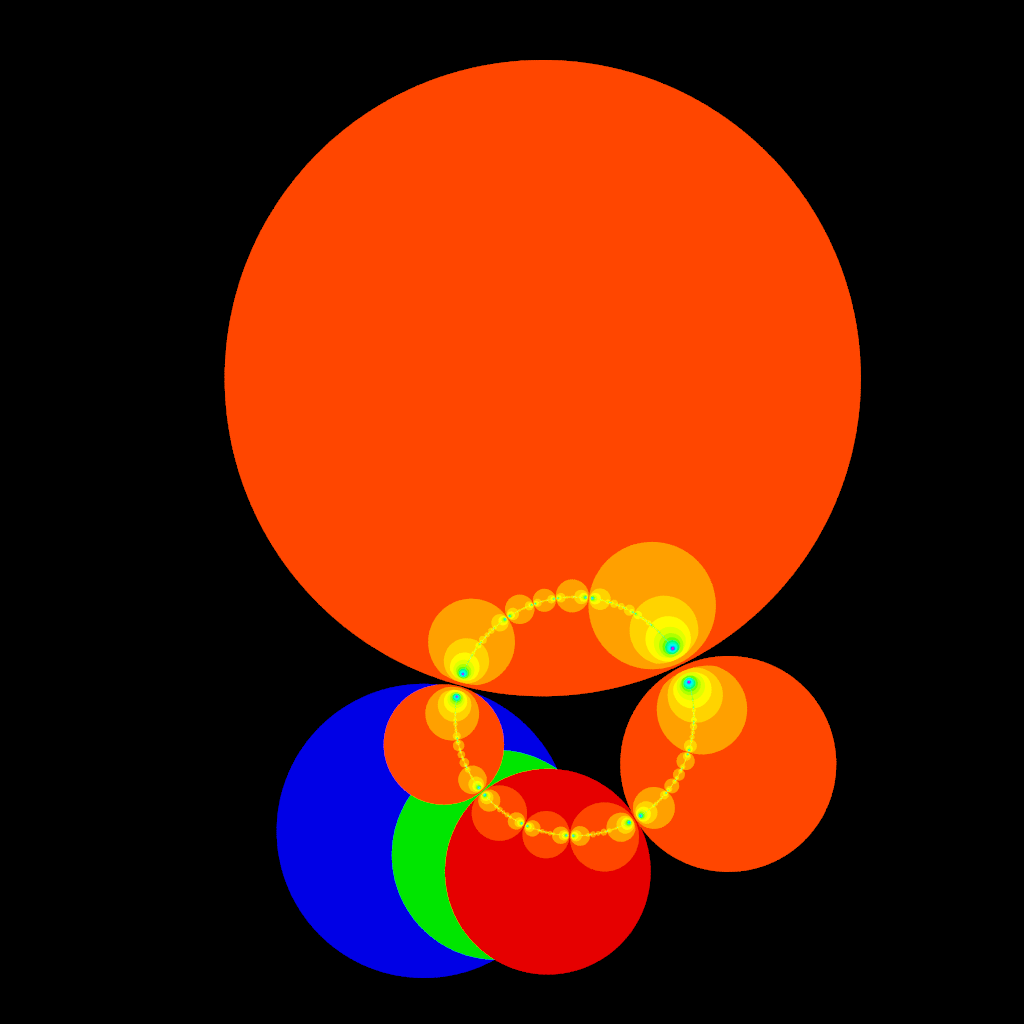
\includegraphics[ height=1.4in, keepaspectratio]{./img/application/2dGen/ellipticOrb.png}
   \subcaption{\textit{Orbit}}
   \label{fig:elliptic2dOrb}
  \end{minipage}
 \hspace*{\fill}
  \caption{\textit{Elliptic generator and a Schottky disk.}}
  \label{fig:elliptic2d}
 \end{minipage}
\end{figure}

\begin{figure}[htbp]
  \begin{minipage}{0.5\hsize}
   \center
   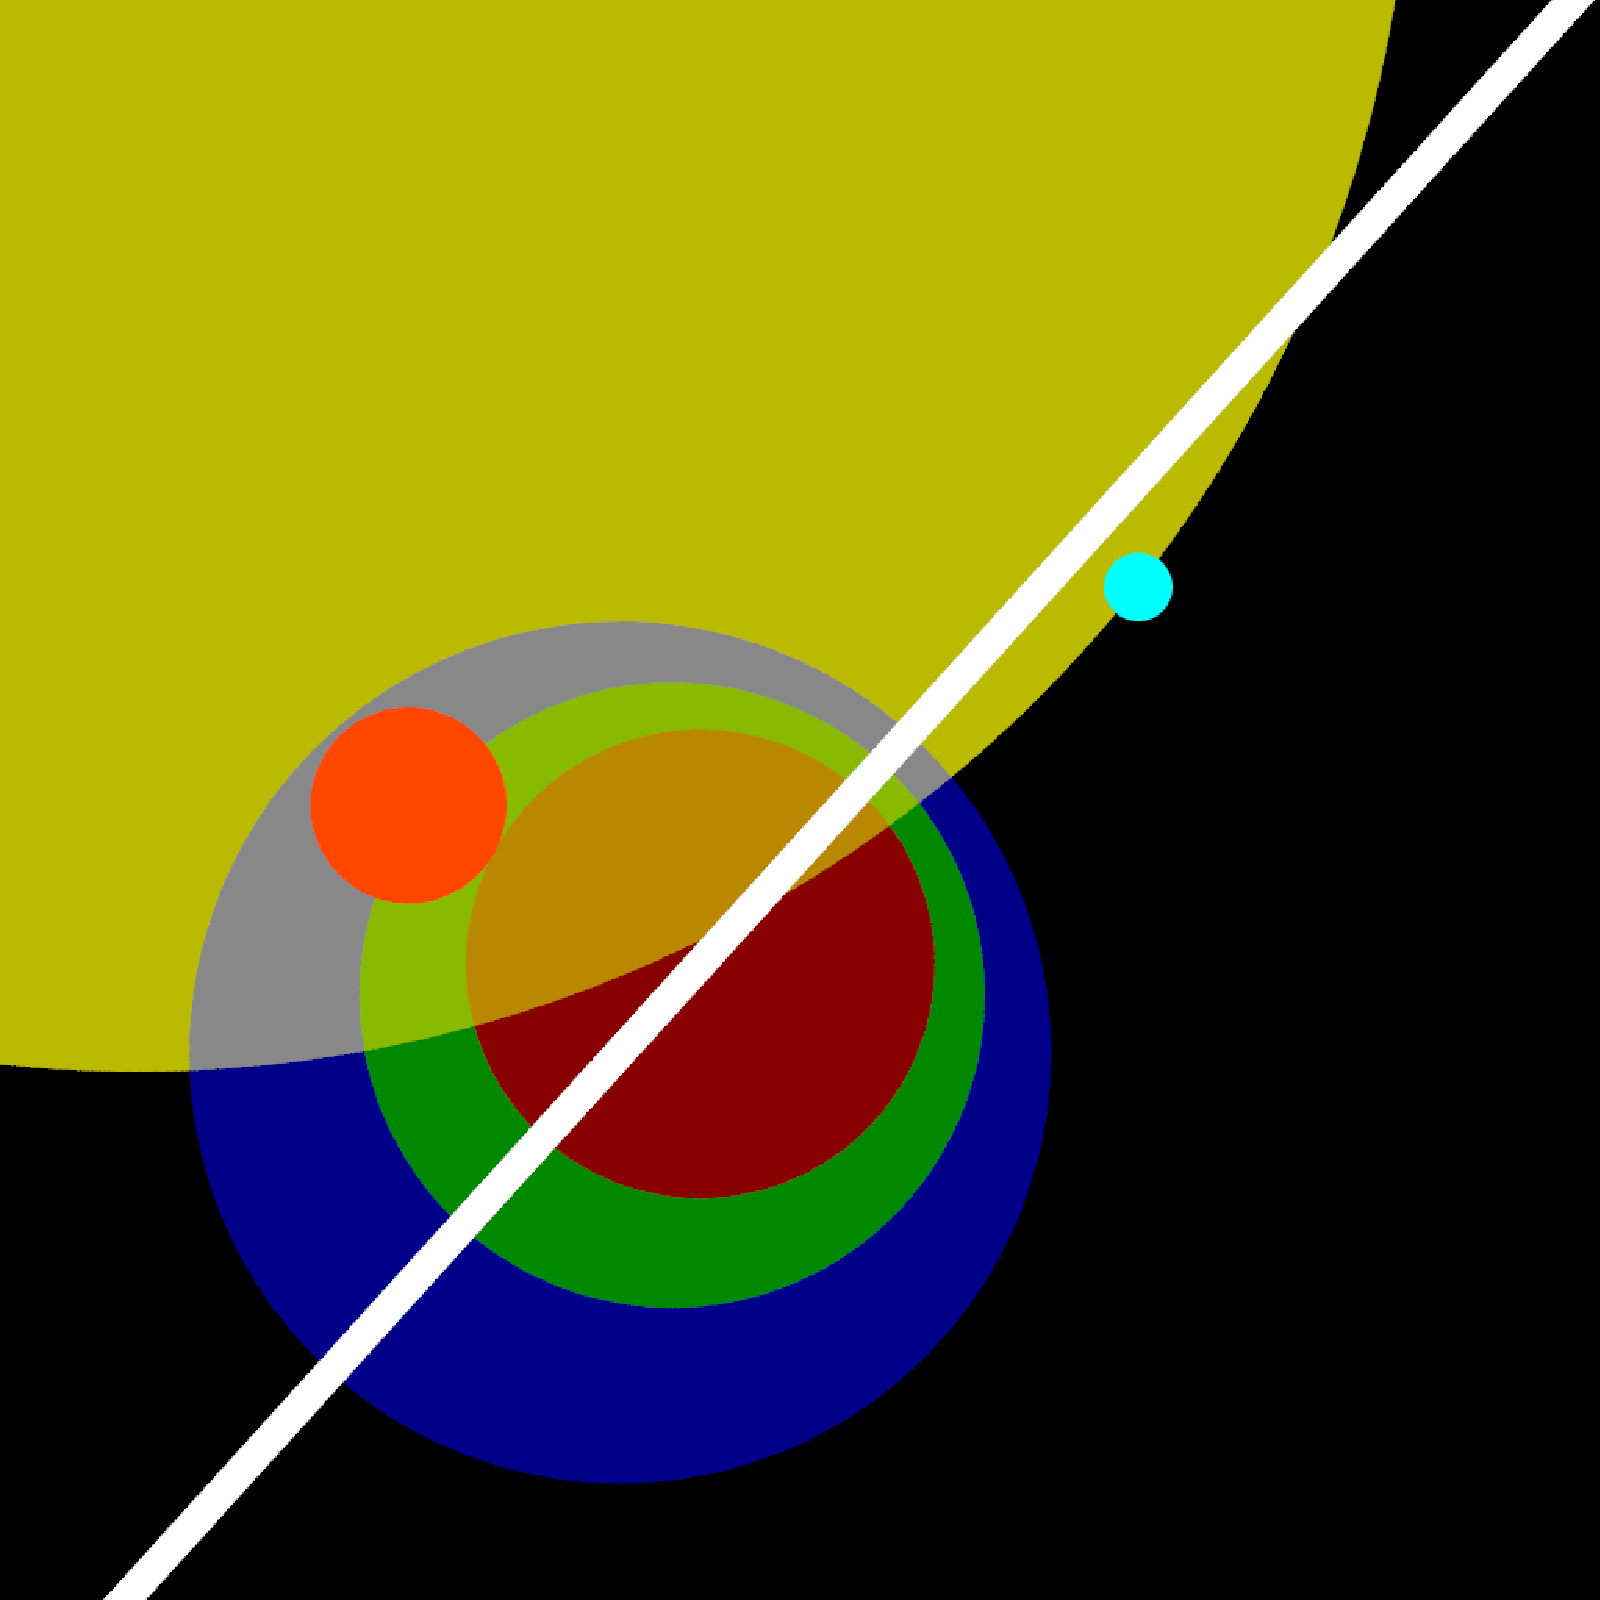
\includegraphics[ height=1.4in, keepaspectratio]{./img/application/2dGen/loxo0.pdf}
   \subcaption{\textit{Generator}}
   \label{fig:loxo2dGen}
  \end{minipage}
 \hspace*{\fill}
  \begin{minipage}{0.5\hsize}
   \center
   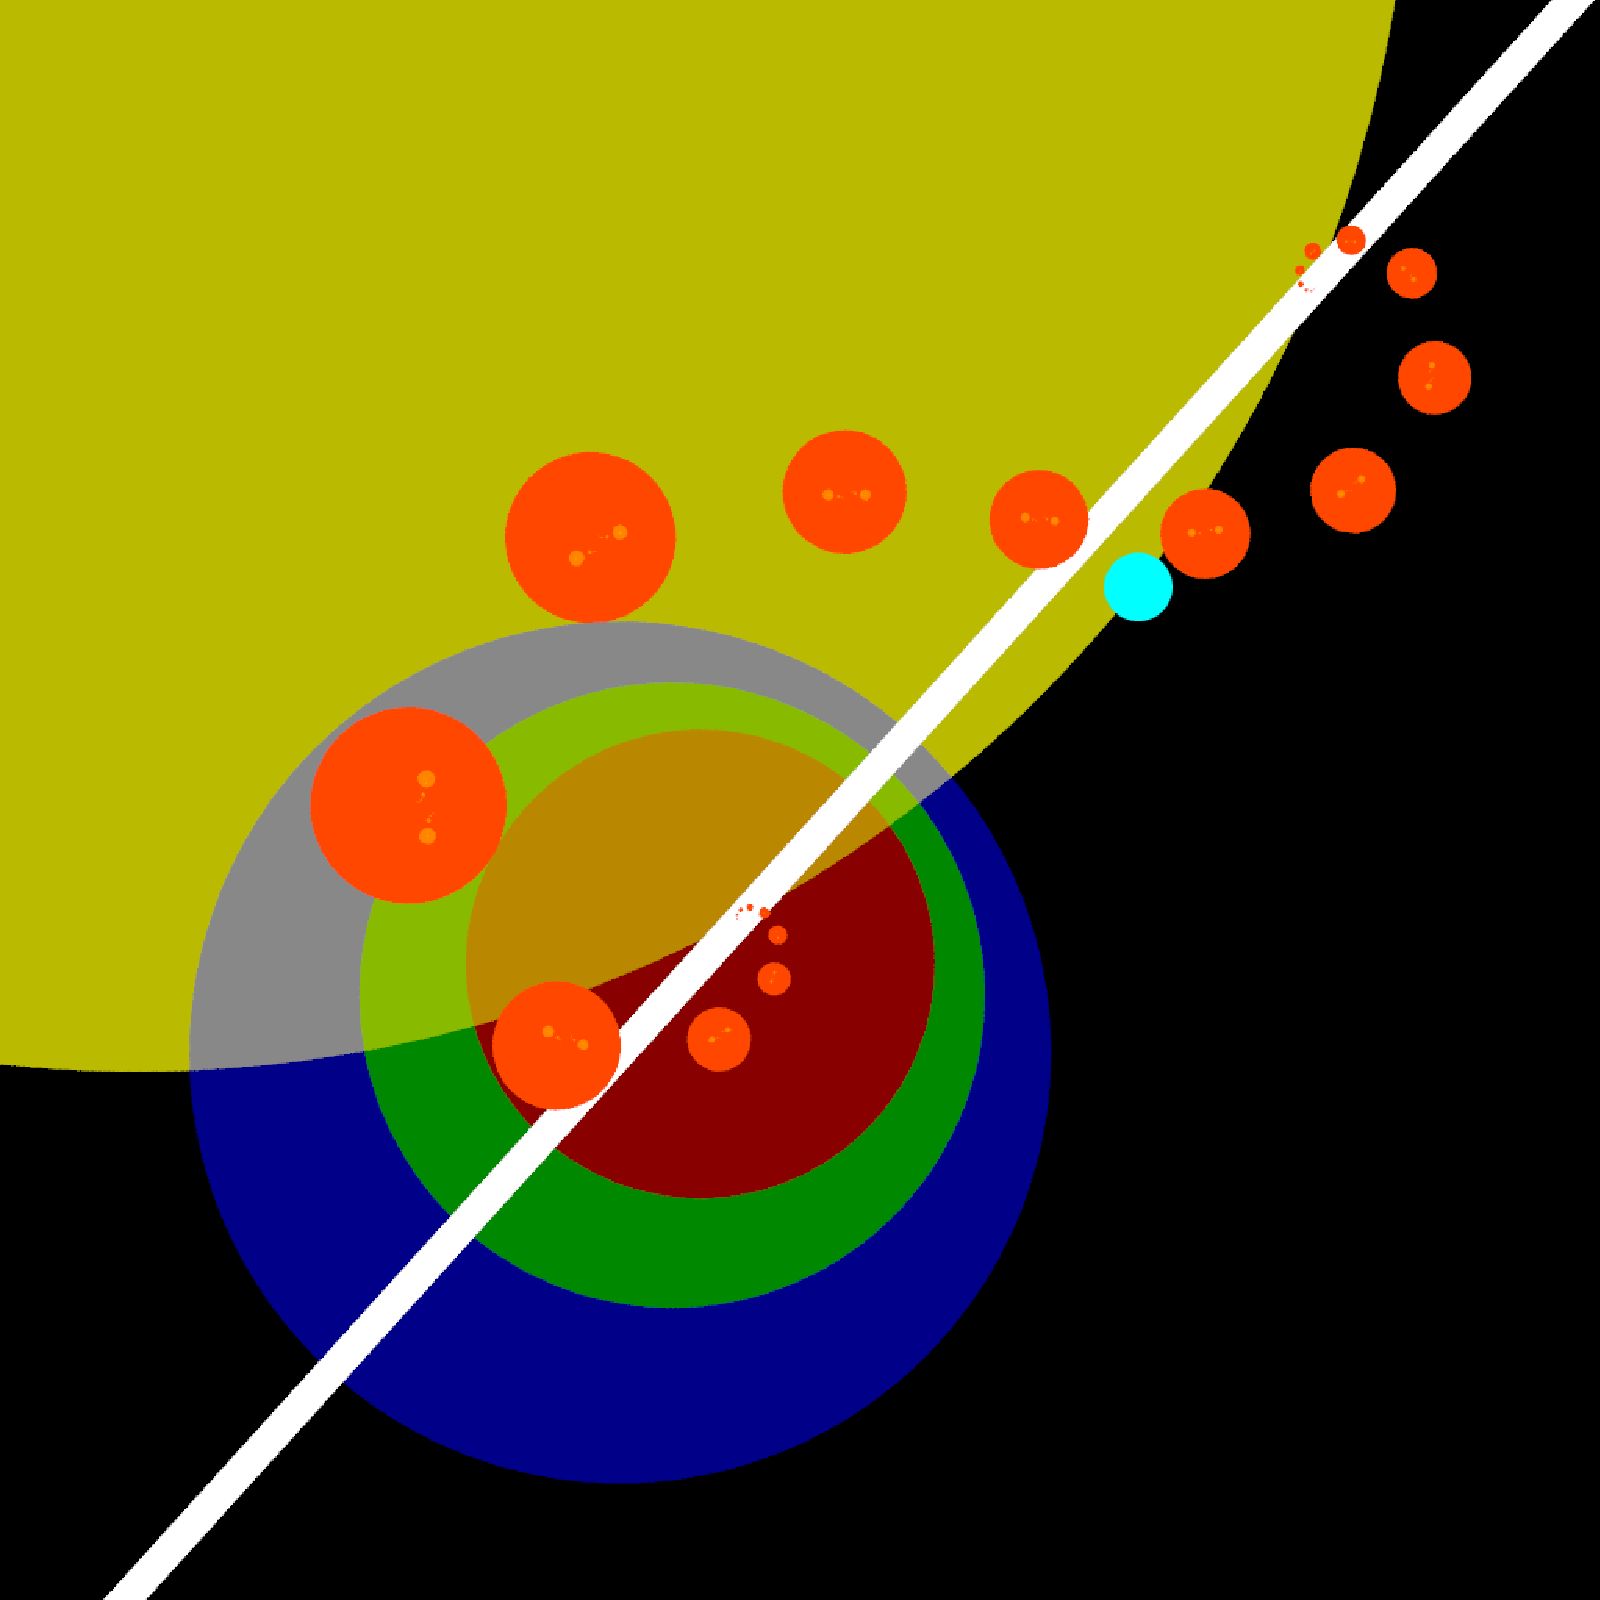
\includegraphics[ height=1.4in, keepaspectratio]{./img/application/2dGen/loxoOrb.pdf}
   \subcaption{\textit{Orbit}}
   \label{fig:loxo2dOrb}
  \end{minipage}
 \hspace*{\fill}
  \caption{\textit{Loxodromic generator and a Schottky disk.}}
  \label{fig:loxodromic2d}
\end{figure}

\noindent\textbf{Inversion in a Circle with Infinite Radius.}
An inversion in a circle with infinite radius is treated as a reflection
over a borderline of half plane. See Figure
\ref{fig:infCircle}\subref{fig:infCircleGen}.
The four inversion circles are lying on the right side, and there is the
orange region on the left side. The region is a half plane, that is, a
disk with infinite radius. Its boundary is colored with a white line.
The orbit is shown in
Figure \ref{fig:infCircle}\subref{fig:infCircleOrb}.
As we can see, the circles are reflected over the white line.

\noindent\textbf{Parallel Translation.}
A composition of reflections over two parallel half planes facing each
other generates a parallel translation. See Figure
\ref{fig:translation2d}\subref{fig:translation2dGen}.
There are two orange half planes on the right and left sides.
The orbit is shown in Figure
\ref{fig:translation2d}\subref{fig:translation2dOrb}.

\noindent\textbf{Rotation.}
A composition of reflections over two crossing half planes generates a
rotation. The generator is shown in Figure
\ref{fig:rotation2d}\subref{fig:rotation2dGen}
The two half planes are crossing. The rotation axis is a crossing point of
white borderlines. The orbit is shown in Figure 
\ref{fig:rotation2d}\subref{fig:rotation2dOrb}.
It has a rotation symmetry and it is an elliptic transformation.
Crossing angle of two borderlines should be
rational angles; otherwise, the orbit will overlap each other.

\noindent\textbf{Composition of Two Circles.}
 Next, we use a composition of inversions in two circles.
 See Figure \ref{fig:hyperbolic2d}\subref{fig:hyperbolic2dGen}.
 There are one inversion disk and three regions colored with red, green,
 and blue.
 We call the boundary of red disk $C1$, 
 the outer circle of green region $C2$, and
 let $C1'$ be the inversion of $C1$ in $C2$.
 The outer circle of the blue region is $C1'$.
 The generator is composed of $C1$, $C2$, and $C1'$.
 While $C1$ and $C2$ have no intersection, the composition of inversions
 in $C1$ and $C2$ represents hyperbolic transformations
 \footnote{\url{https://www.shadertoy.com/view/MsScWW}}.
 The orbit is shown in Figure
 \ref{fig:hyperbolic2d}\subref{fig:hyperbolic2dOrb}.
 The orbit of the disk converges to two fixed points.
 We compose the map $G$ as follows.
 The prefix $I$ represents an inversion, for example, $I_{C1}$ represents
 an inversion in $C1$.
 \begin{align*}
  G =
  \begin{cases}
   I_{C2} \circ I_{C1} & (\text{The point is inside of } C1) \\
   I_{C1} \circ I_{C2} & (\text{The point is outside of }C1')
  \end{cases}
 \end{align*}
 In the process of IIS, we can transform the point to the fundamental
 domain by applying $G$ repeatedly.
 The fundamental domain of this type of generators is the blue and green
 area in Figure \ref{fig:hyperbolic2d}\subref{fig:hyperbolic2dGen}.

 Then, we displace $C1$.
 When $C1$ and $C2$ are kissing as shown in Figure 
 \ref{fig:parabolic2d}\subref{fig:parabolic2dGen},
 this generator becomes a parabolic transformation
 \footnote{\url{https://www.shadertoy.com/view/XsBcDD}}.
 The fixed points overlap each other, and the orbit converges to the
 point as shown in Figure \ref{fig:parabolic2d}\subref{fig:parabolic2dOrb}.

 When $C1$ and $C2$ are crossing as in Figure \ref{fig:elliptic2d},
 the generator becomes an elliptic transformation.
 The orbit is as shown in Figure \ref{fig:elliptic2d}\subref{fig:elliptic2dOrb}.
 The disks are rotated around crossing line.
 Note that a crossing angle of $C1$ and $C2$ should be rational angles;
 otherwise, the orbit of the disks will overlap each other.

\noindent\textbf{Loxodromic.}
 We can twist the orbit by adding another two inversions.
 See Figure \ref{fig:loxodromic2d}\subref{fig:loxo2dGen}.
 The yellow disk and the white line are added to the hyperbolic generator.
 The white line is a line with two centers of $C1$ and $C2$.
 We call the line $L$, the boundary of the yellow disk $C3$, and
 light blue point $P$.
 $P$ is a user-defined control point, and the circle $C3$ is determined
 by three points, one is the point $P$, and the others are inversions
 of $P$ in $C1$ and $C2$.
 $L$ and $C3$ are perpendicular to $C1$ and $C2$.
 Thus, a composition of the reflection over $L$ and the inversion in $C3$
 represents a rotation, and
 the orbit of the group is twisted as shown in Figure
 \ref{fig:loxodromic2d}\subref{fig:loxo2dOrb}. This is a loxodromic
 transformation\footnote{\url{https://www.shadertoy.com/view/lsSyDW}}.
 The map $G$ is as follows.
 \begin{align*}
  G =
  \begin{cases}
   (I_{C2} \circ I_{C1}) \circ (I_{C3} \circ I_L) & (\text{The point is inside of } C1) \\
   (I_L \circ I_{C3}) \circ (I_{C1} \circ I_{C2}) & (\text{The point is outside of }C1')
  \end{cases}
 \end{align*}

\subsubsection{Three Dimensionanl Generators}

\begin{figure}[h!tbp]
 \begin{minipage}[t]{0.5\hsize}
  \begin{minipage}{0.25\hsize}
   \center
   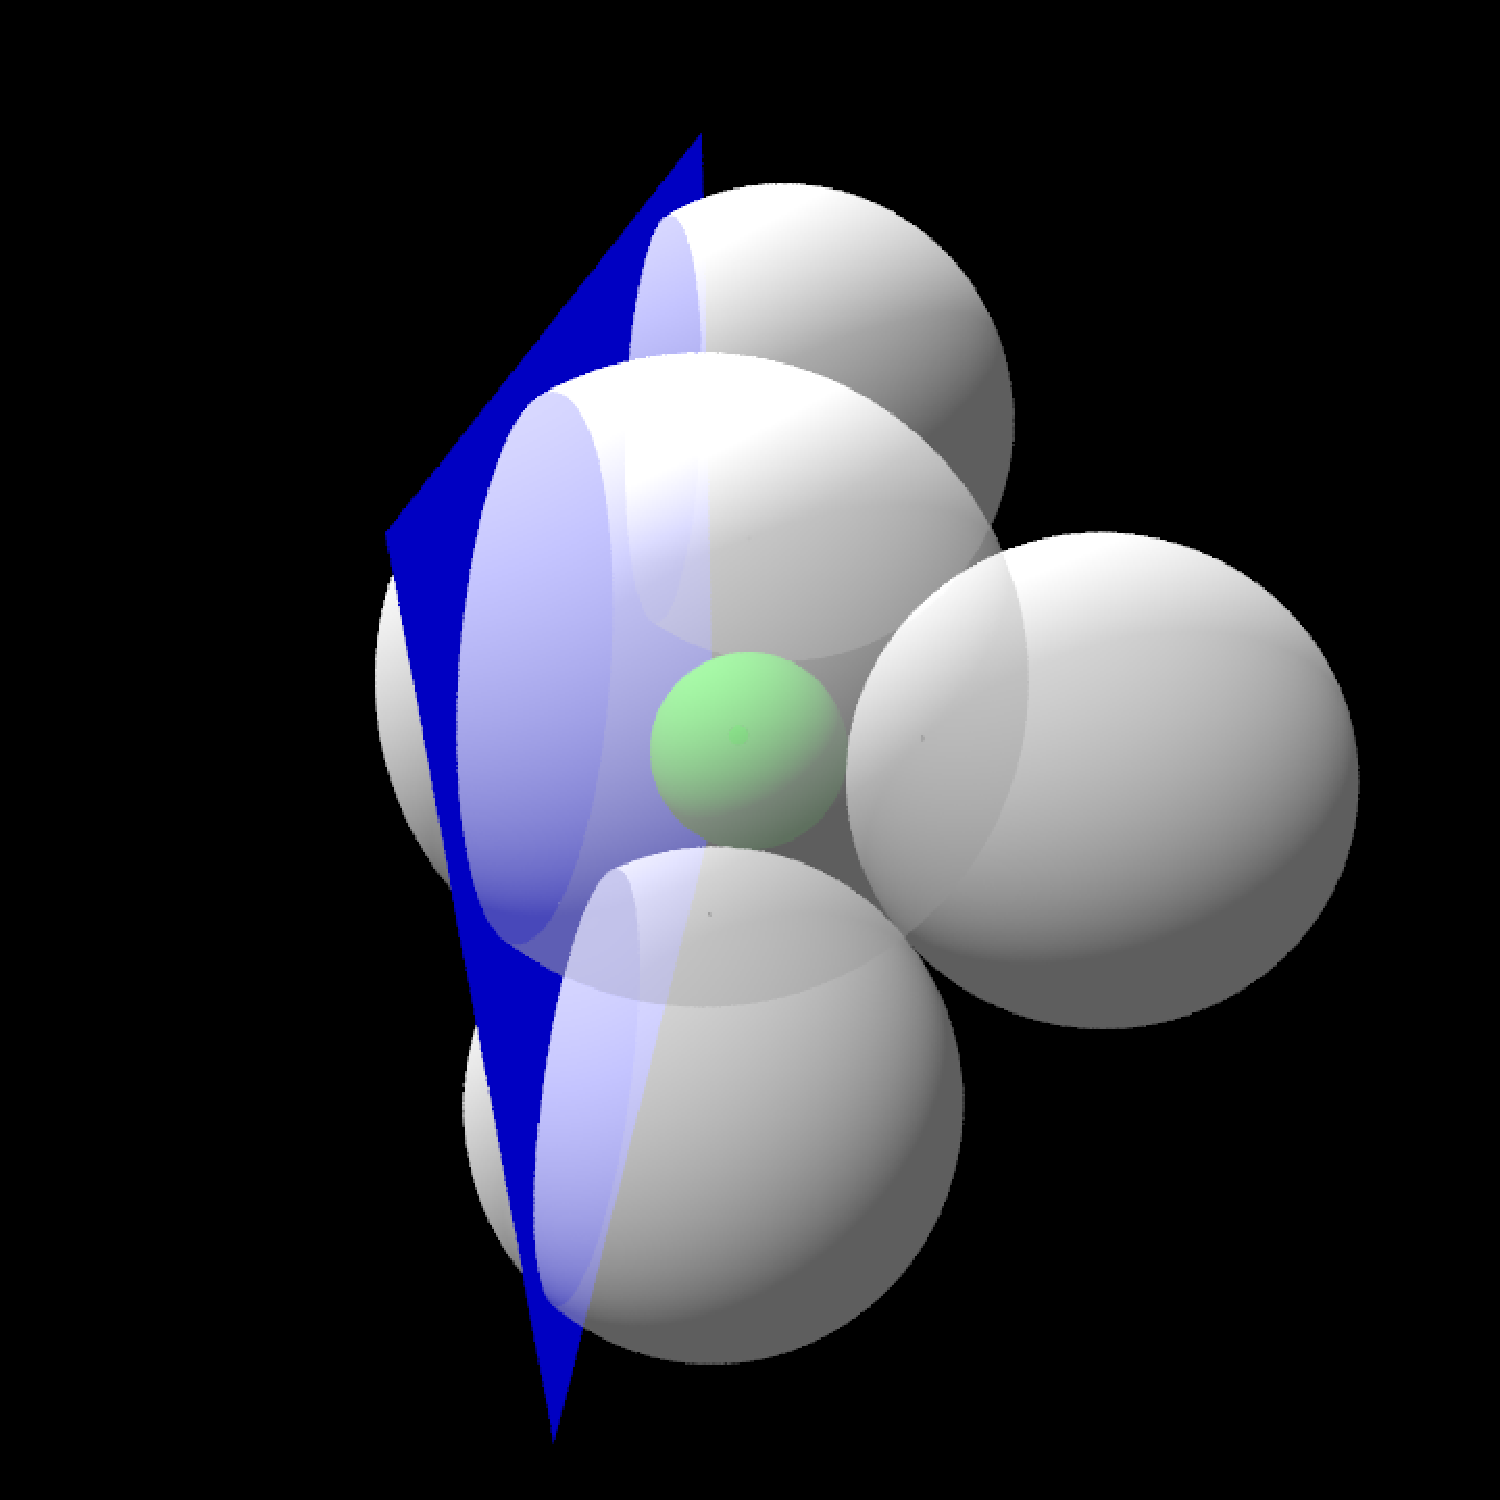
\includegraphics[width=1.4in, height=1.4in, keepaspectratio]{./img/application/3dGen/infSphereGen.pdf}
   \subcaption{\textit{Generator}}
   \label{fig:infSphereGen}
  \end{minipage}
  \hspace*{\fill}
  \begin{minipage}{0.25\hsize}
   \center
   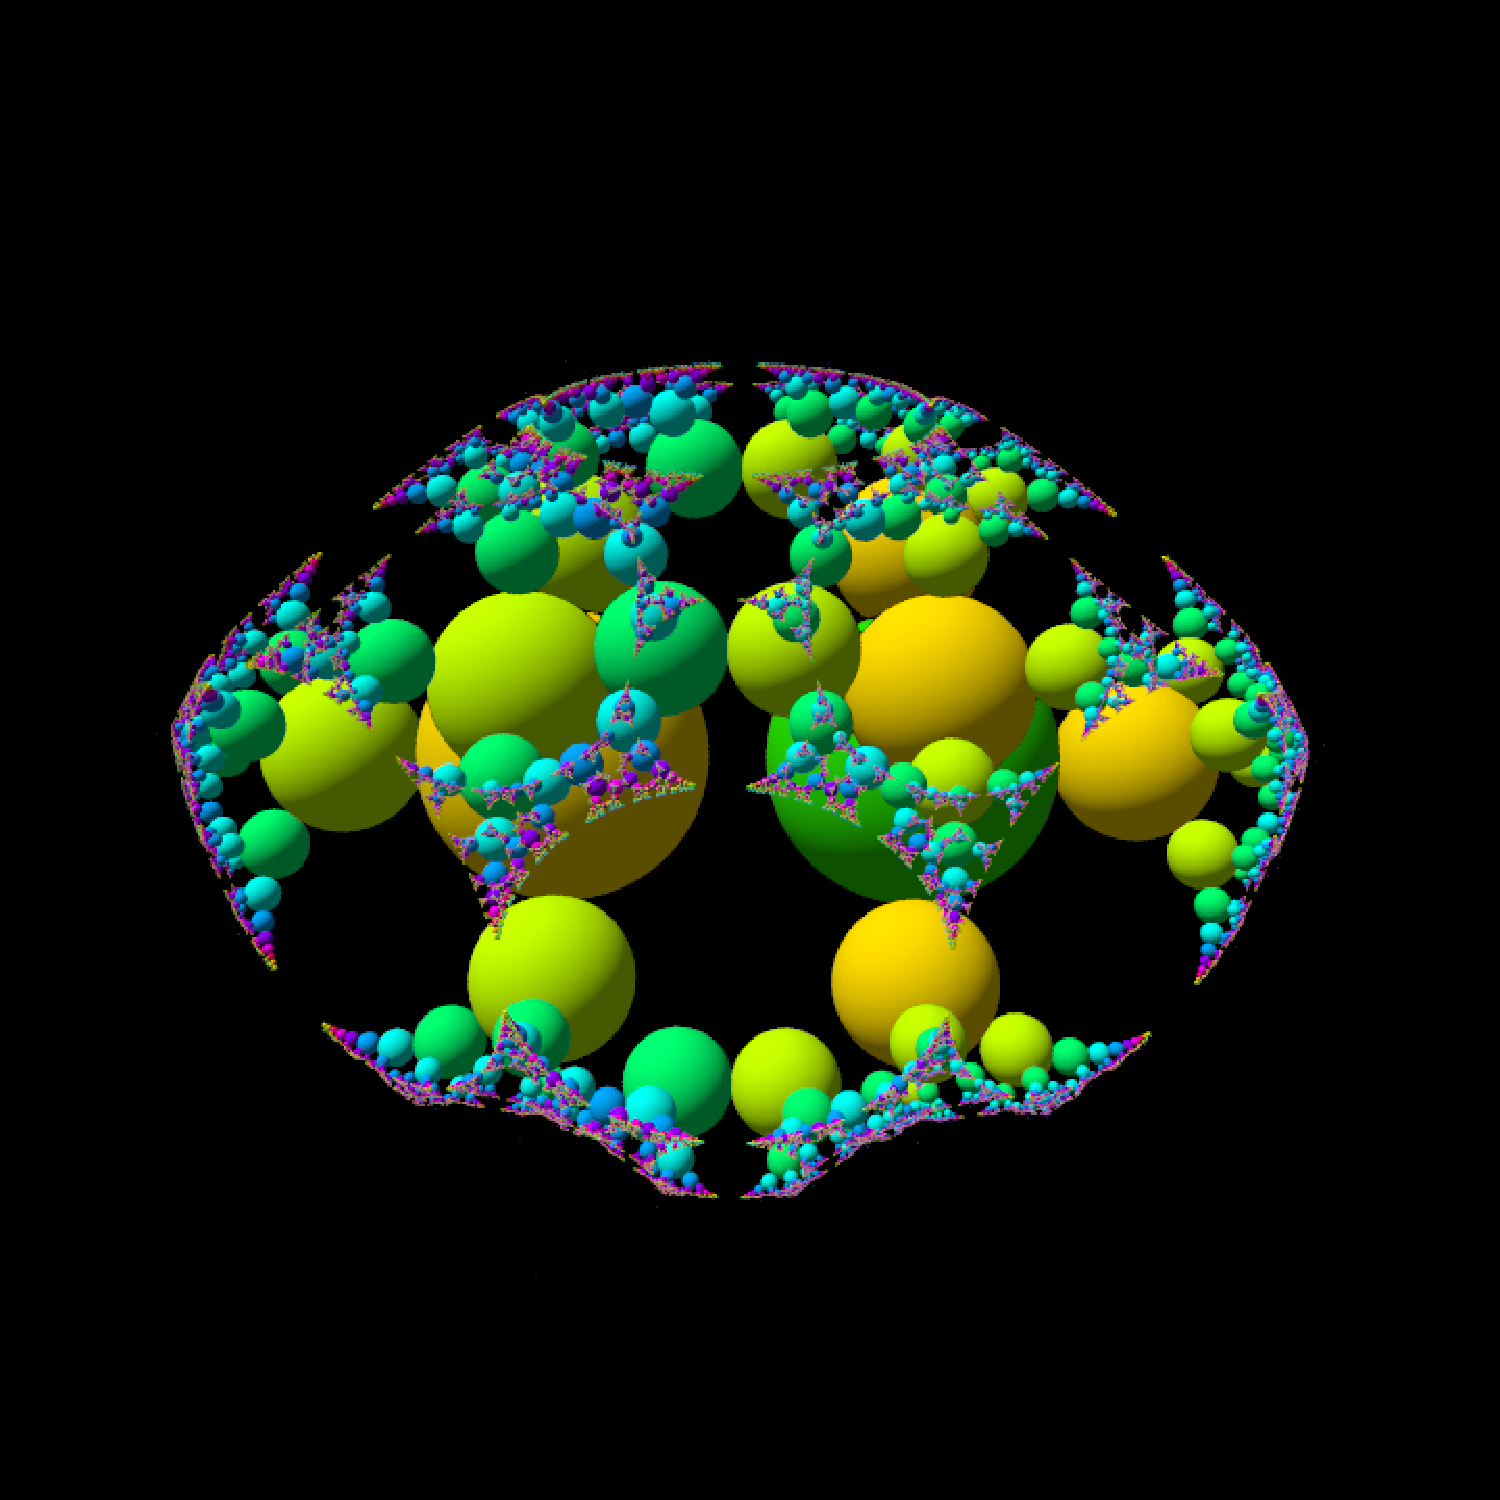
\includegraphics[width=1.4in, height=1.4in, keepaspectratio]{./img/application/3dGen/infSphereOrbit.pdf}
   \subcaption{\textit{Orbit}}
   \label{fig:infSphereOrb}
  \end{minipage}
  \hspace*{\fill}
  \caption{\textit{Inversion in the sphere with infinite radius, four
  Schottky spheres, and a base sphere.}}
  \label{fig:infSphere}
 \end{minipage}
 \hspace*{\fill}
 \begin{minipage}[t]{0.5\hsize}
  \begin{minipage}{0.25\hsize}
   \center
   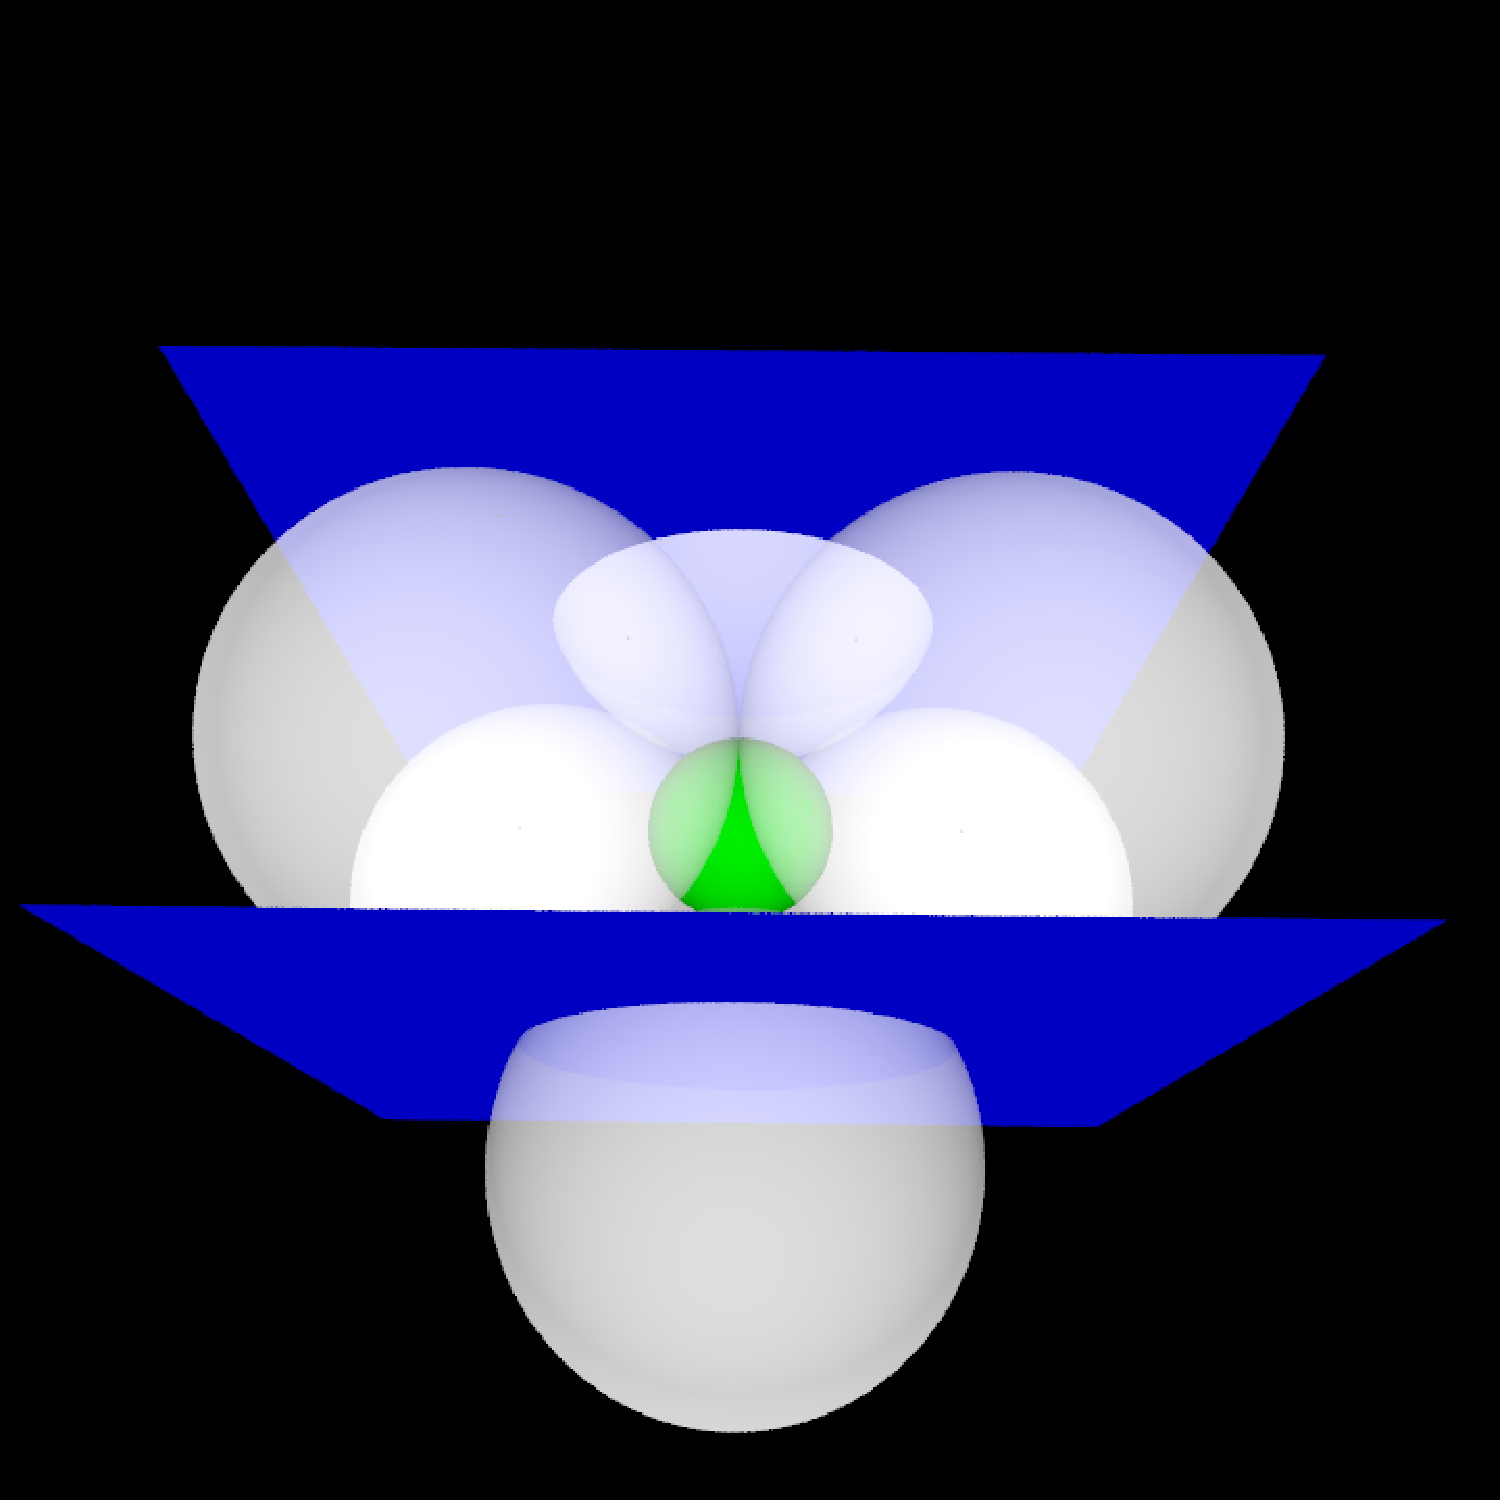
\includegraphics[width=1.4in, height=1.4in, keepaspectratio]{./img/application/3dGen/translationGen.pdf}
   \subcaption{\textit{Generator}}
   \label{fig:translation3dGen}
  \end{minipage}
  \hspace*{\fill}
 \begin{minipage}{0.25\hsize}
  \center
  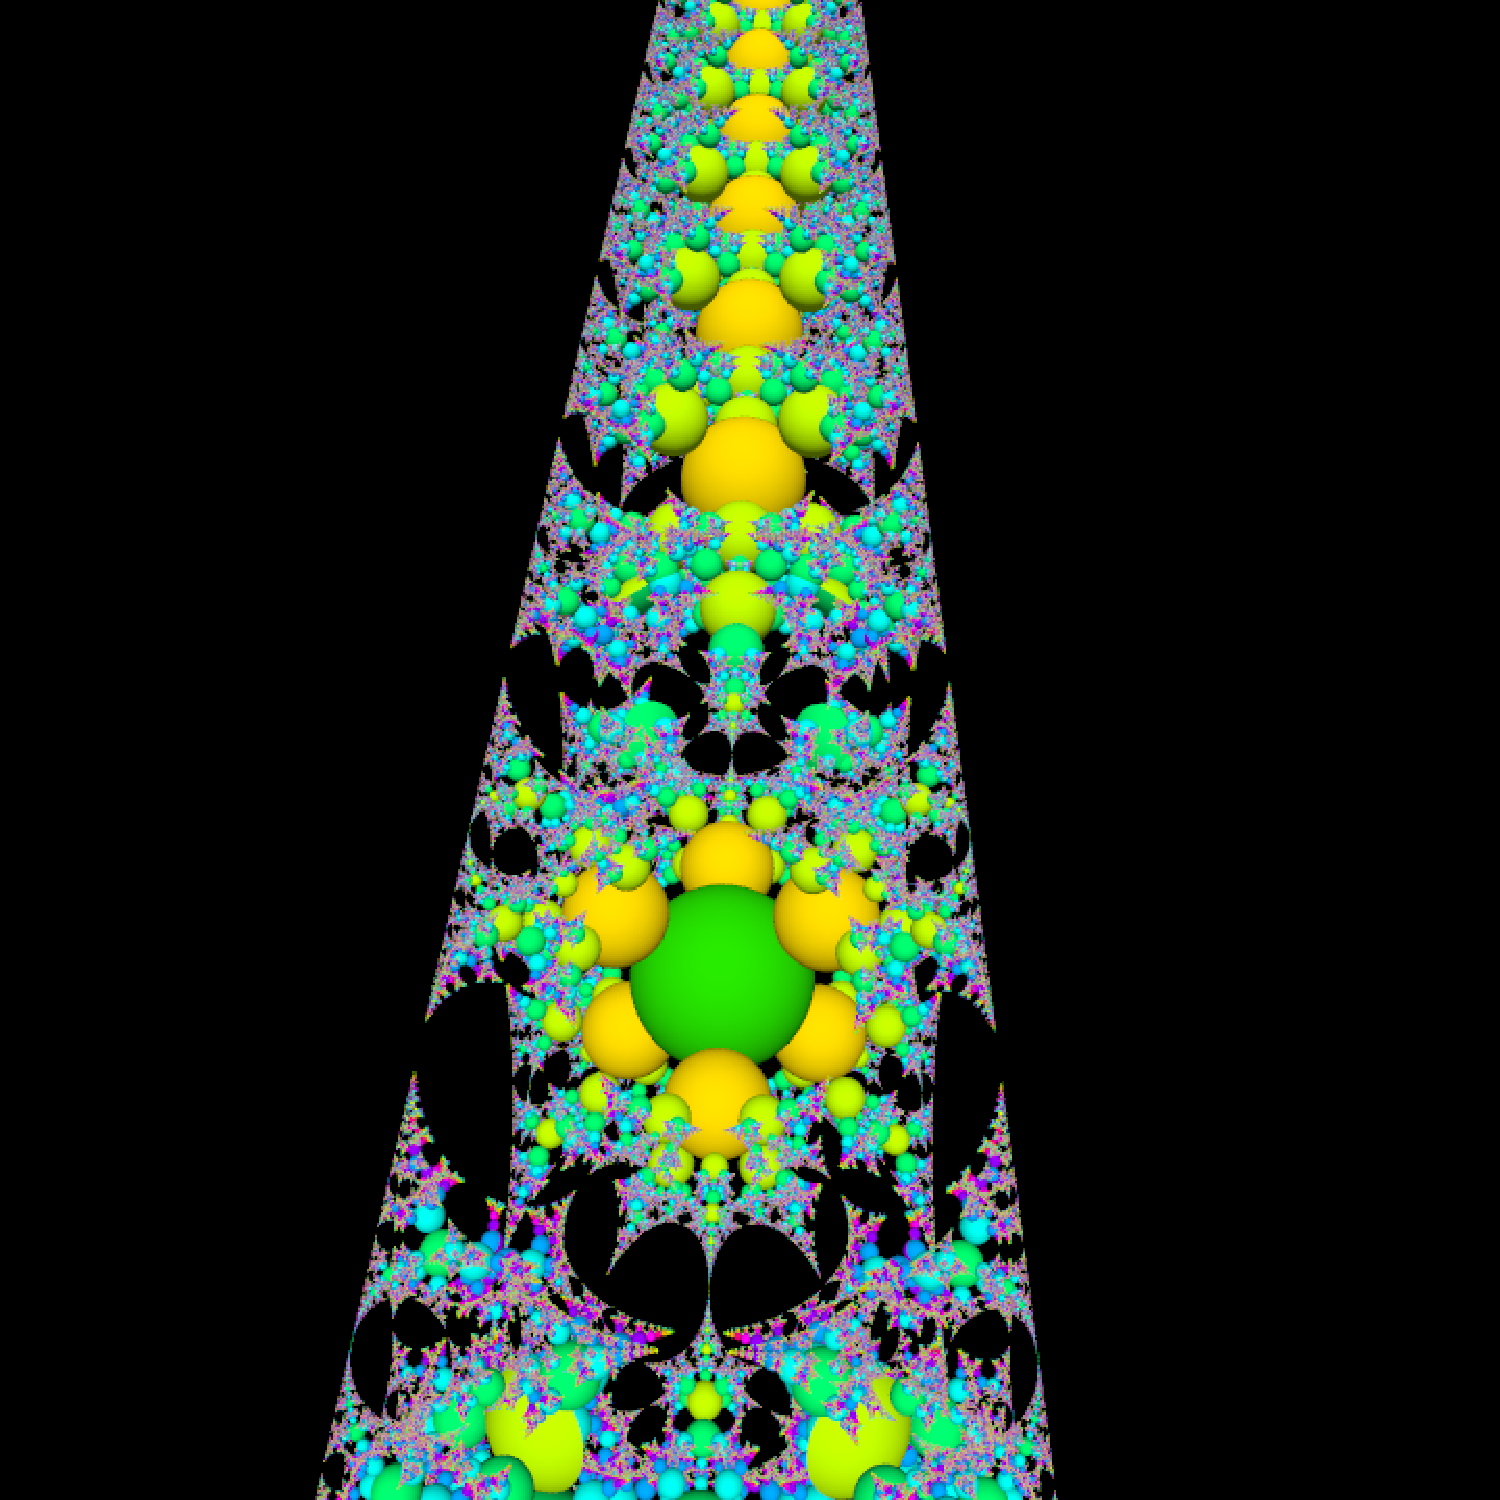
\includegraphics[width=1.4in, height=1.4in, keepaspectratio]{./img/application/3dGen/translationOrbit.pdf}
  \subcaption{\textit{Orbit}}
    \label{fig:translation3dOrb}
 \end{minipage}
  \hspace*{\fill}
  \caption{\textit{Parallel translation generator, six Schottky spheres
  and a base sphere.}}
  \label{fig:translation3d}
 \end{minipage}
\end{figure}

\begin{figure}[h!tbp]
 \begin{minipage}[t]{0.5\hsize}
  \begin{minipage}{0.25\hsize}
   \center
    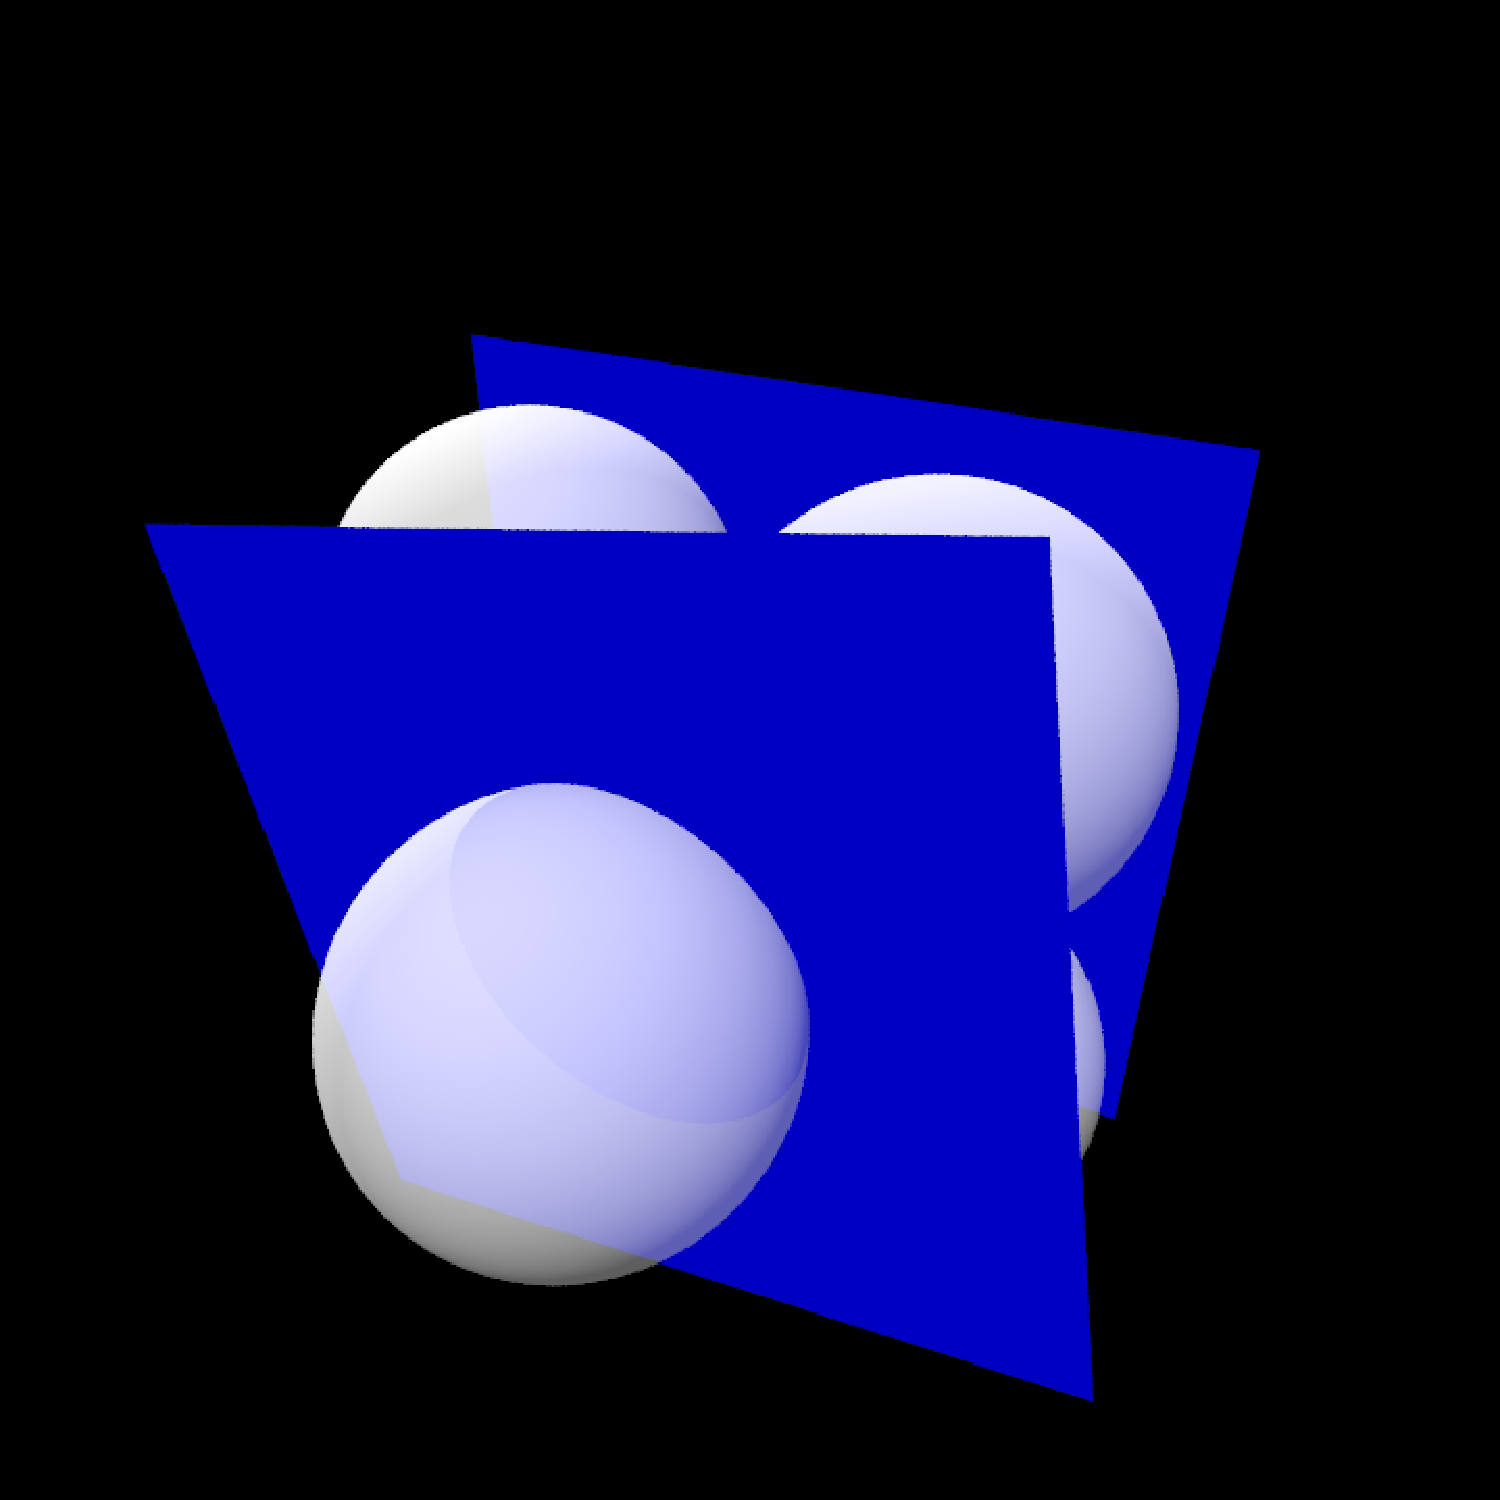
\includegraphics[width=1.4in, height=1.4in, keepaspectratio]{./img/application/3dGen/compParabolicGen.pdf}
    \subcaption{\textit{Generator}}
    \label{fig:compParabolicGen}
  \end{minipage}
  \hspace*{\fill}
  \begin{minipage}{0.25\hsize}
   \center
   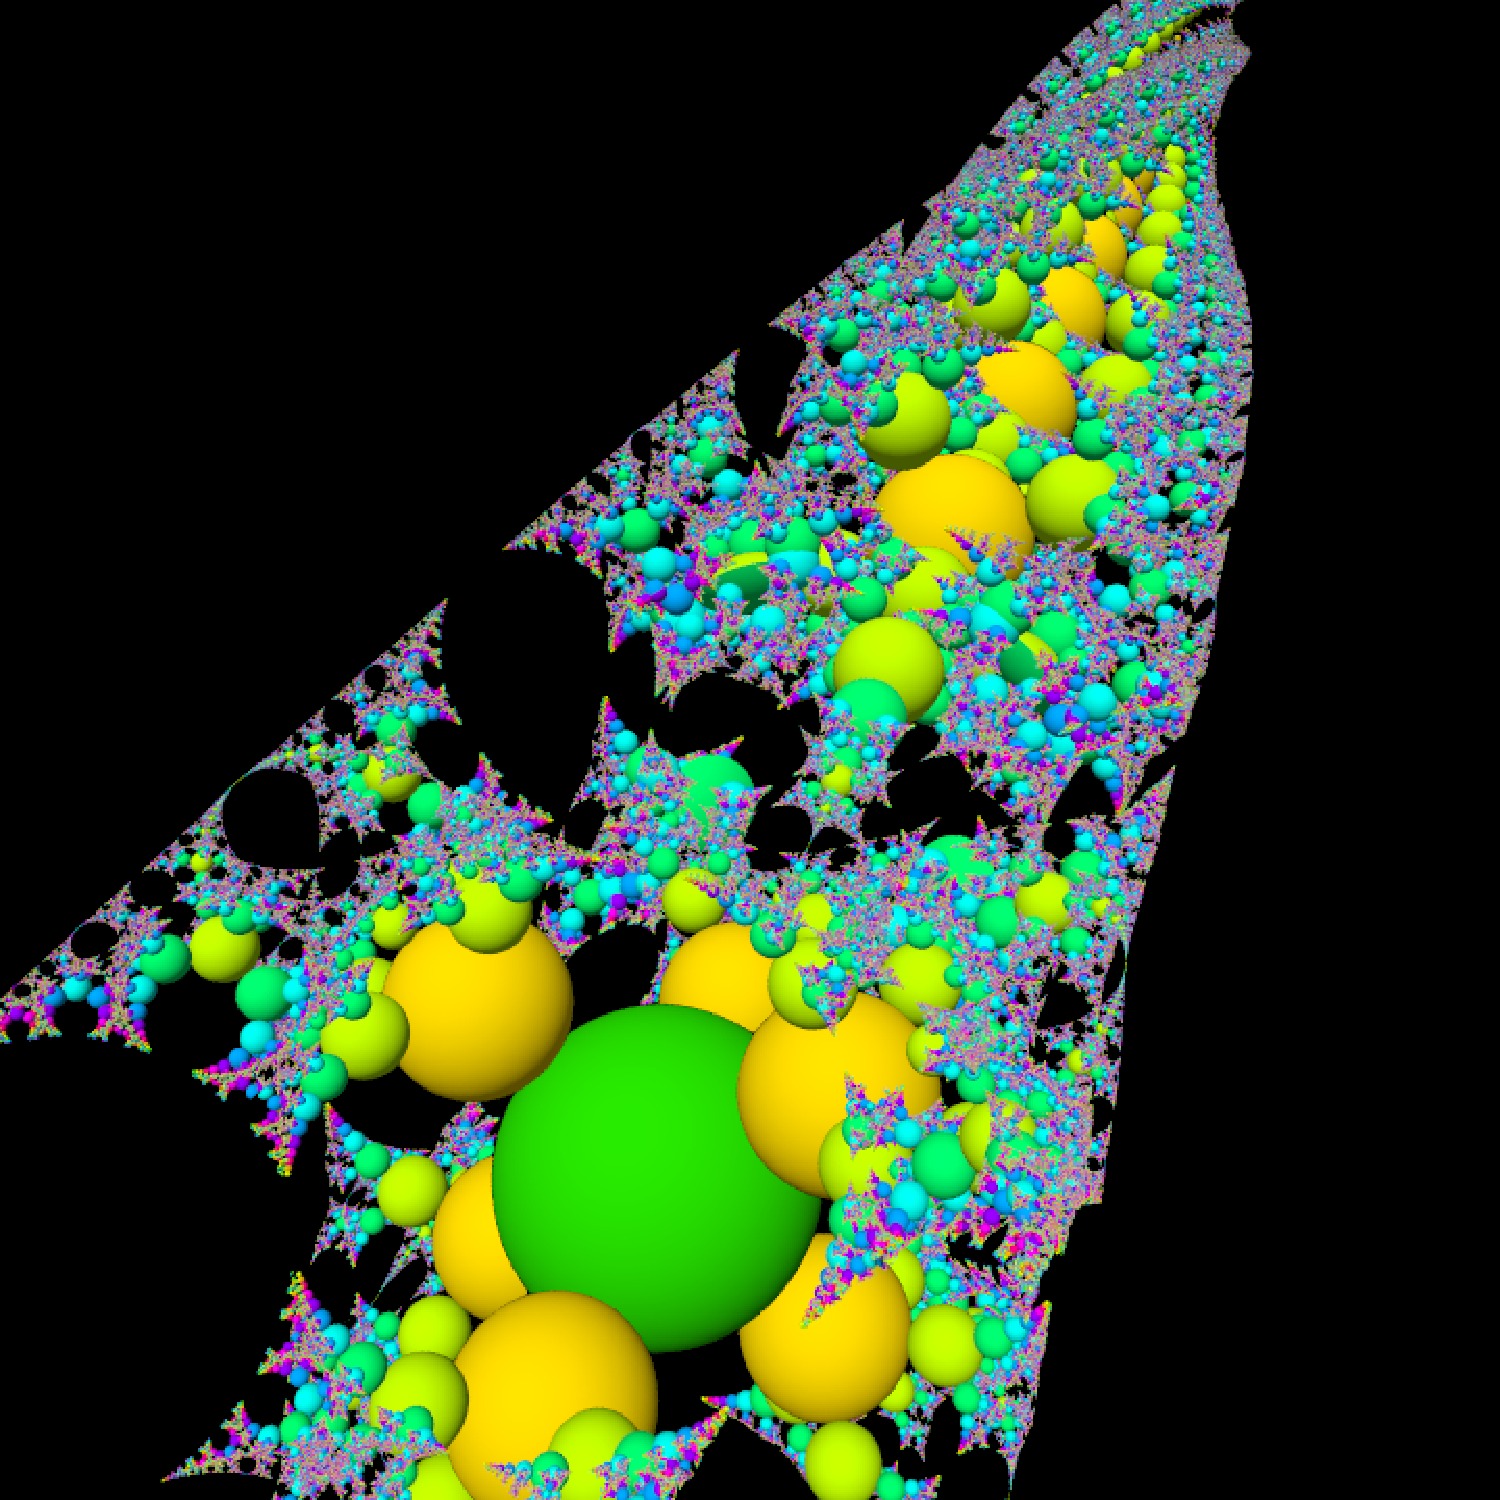
\includegraphics[width=1.4in, height=1.4in, keepaspectratio]{./img/application/3dGen/compParabolicOrb.pdf}
   \subcaption{\textit{Orbit}}
   \label{fig:compParabolicOrb}
  \end{minipage}
  \hspace*{\fill}
  \caption{\textit{Compound parabolic generator, six \\Schottky spheres
  and a base sphere.}}
  \label{fig:compParabolic}
 \end{minipage}
 \hspace*{\fill}
 \begin{minipage}[t]{0.5\hsize}
  \begin{minipage}{0.25\hsize}
   \center
   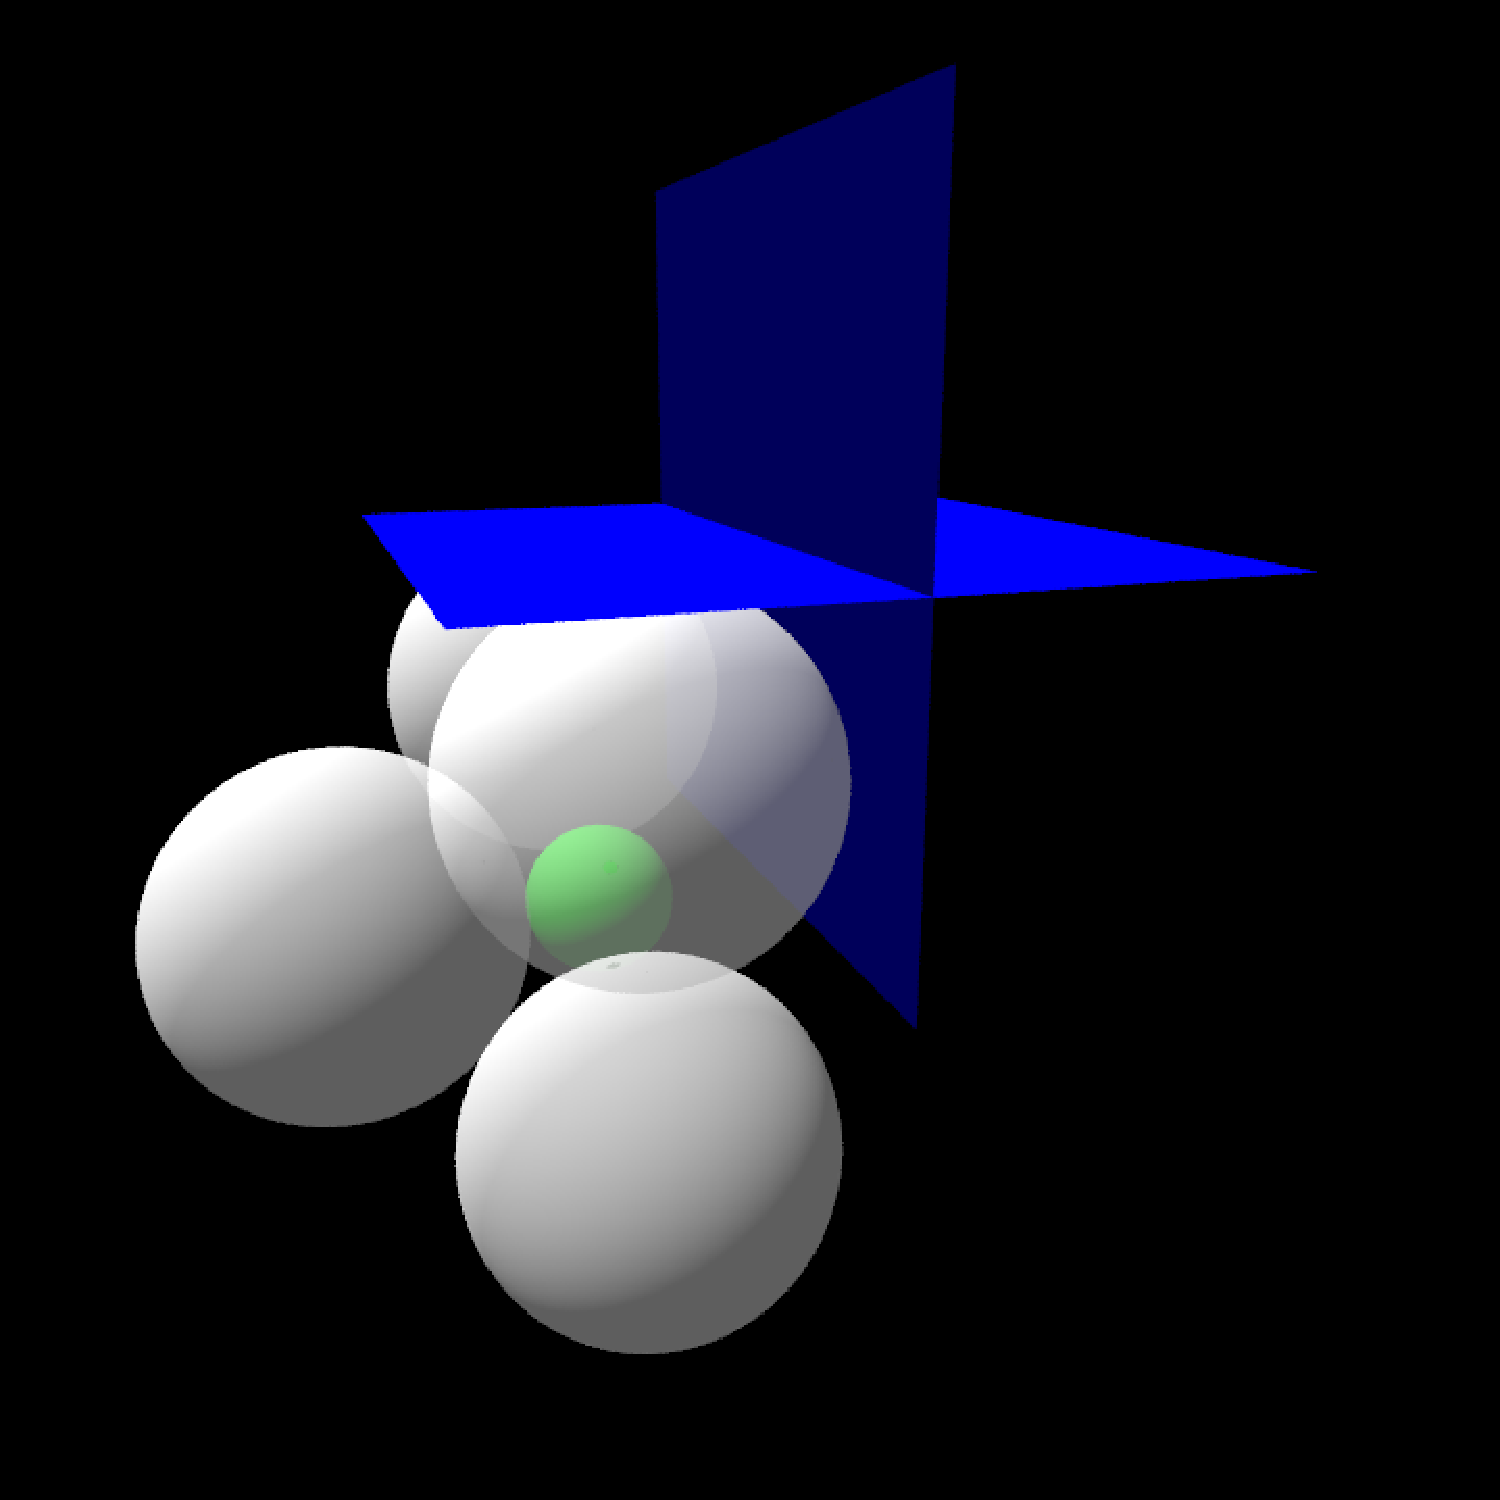
\includegraphics[width=1.4in, height=1.4in, keepaspectratio]{./img/application/3dGen/rotationGen.pdf}
   \subcaption{\textit{Generator}}
   \label{fig:rotationGen}
  \end{minipage}
  \hspace*{\fill}
  \begin{minipage}{0.25\hsize}
   \center
   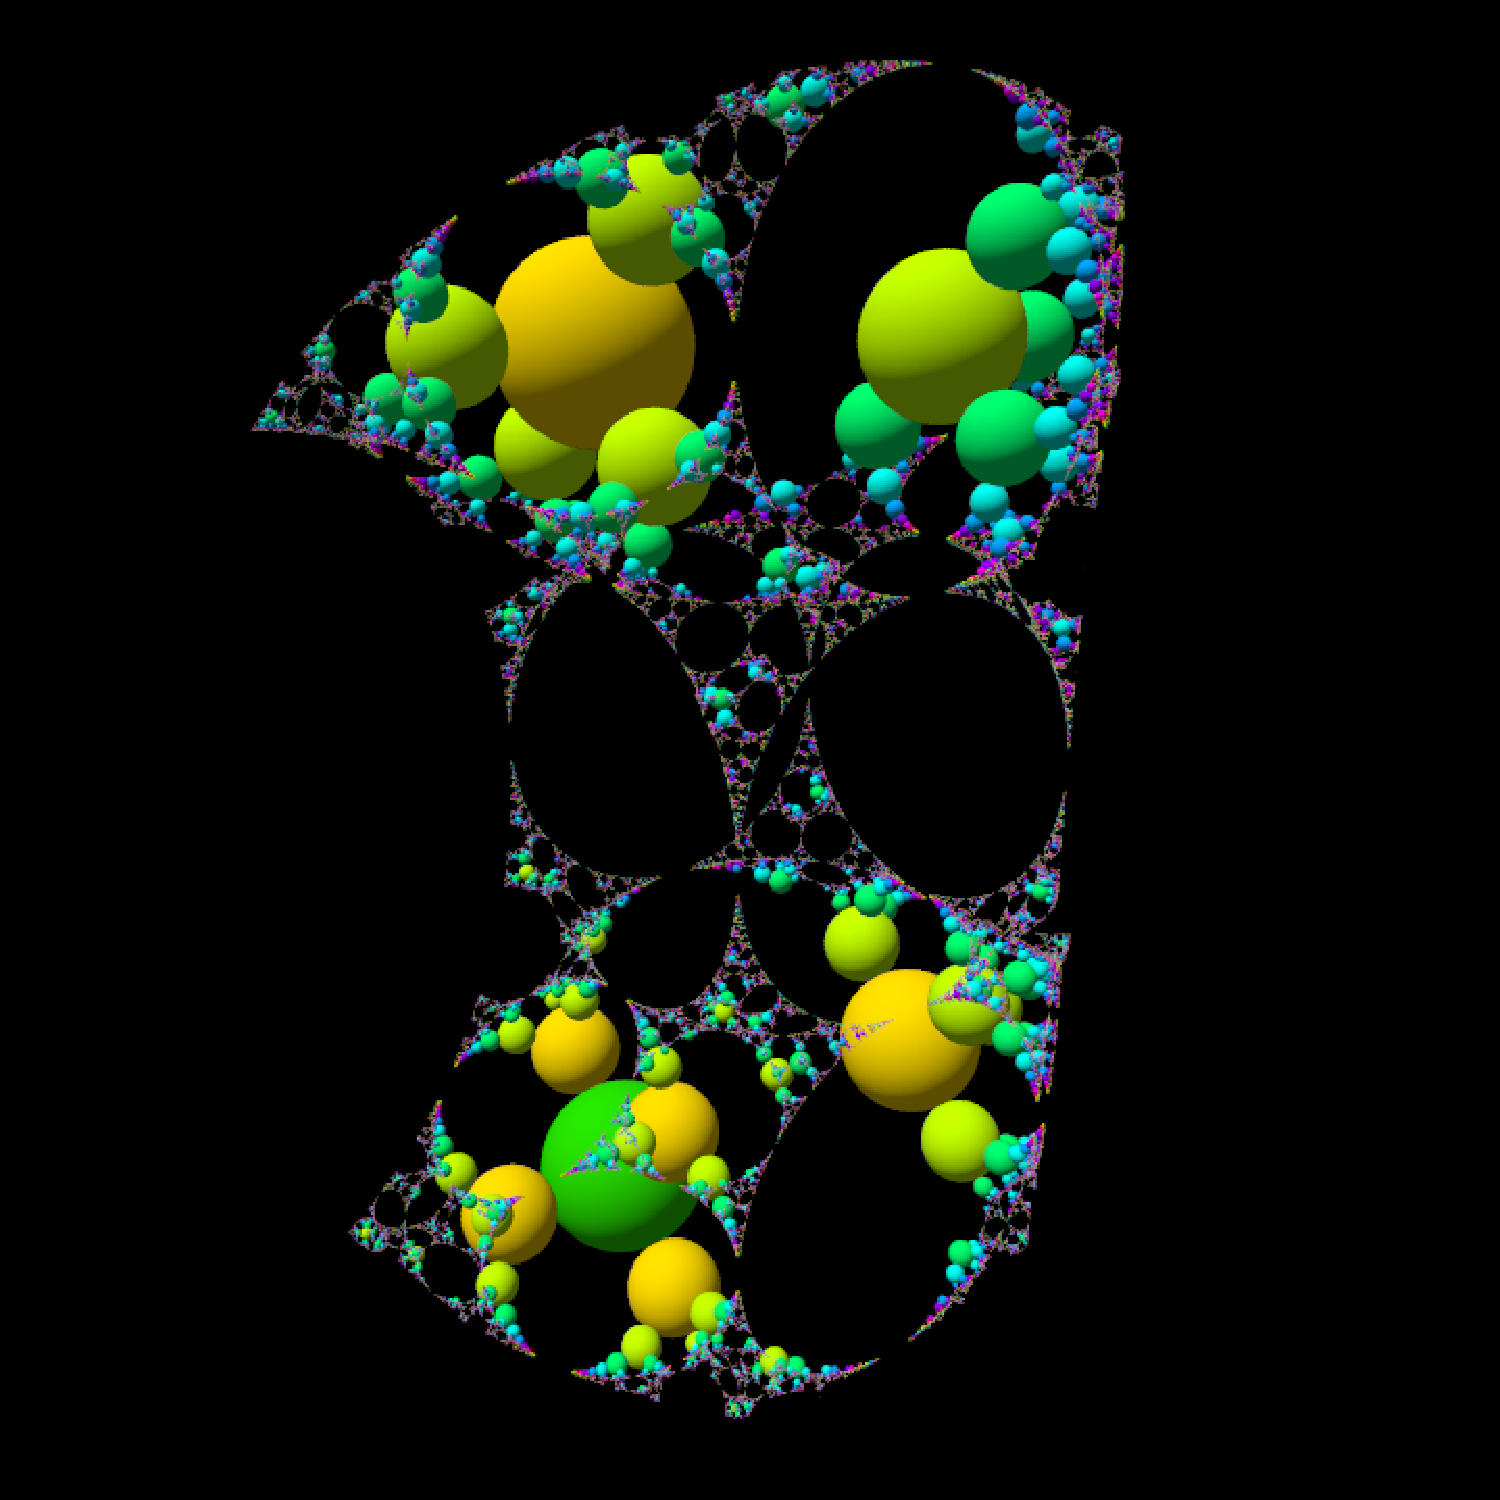
\includegraphics[width=1.4in, height=1.4in, keepaspectratio]{./img/application/3dGen/rotationOrb.pdf}
   \subcaption{\textit{Orbit}}
   \label{fig:rotationOrb}
  \end{minipage}
  \hspace*{\fill}
  \caption{\textit{Rotation generator, four Schottky spheres, and a base
  sphere.}}
  \label{fig:rotation3d}
 \end{minipage}
\end{figure}

\begin{figure}[h!tbp]
 \begin{minipage}{0.5\hsize}
  \begin{minipage}{0.25\hsize}
   \center
   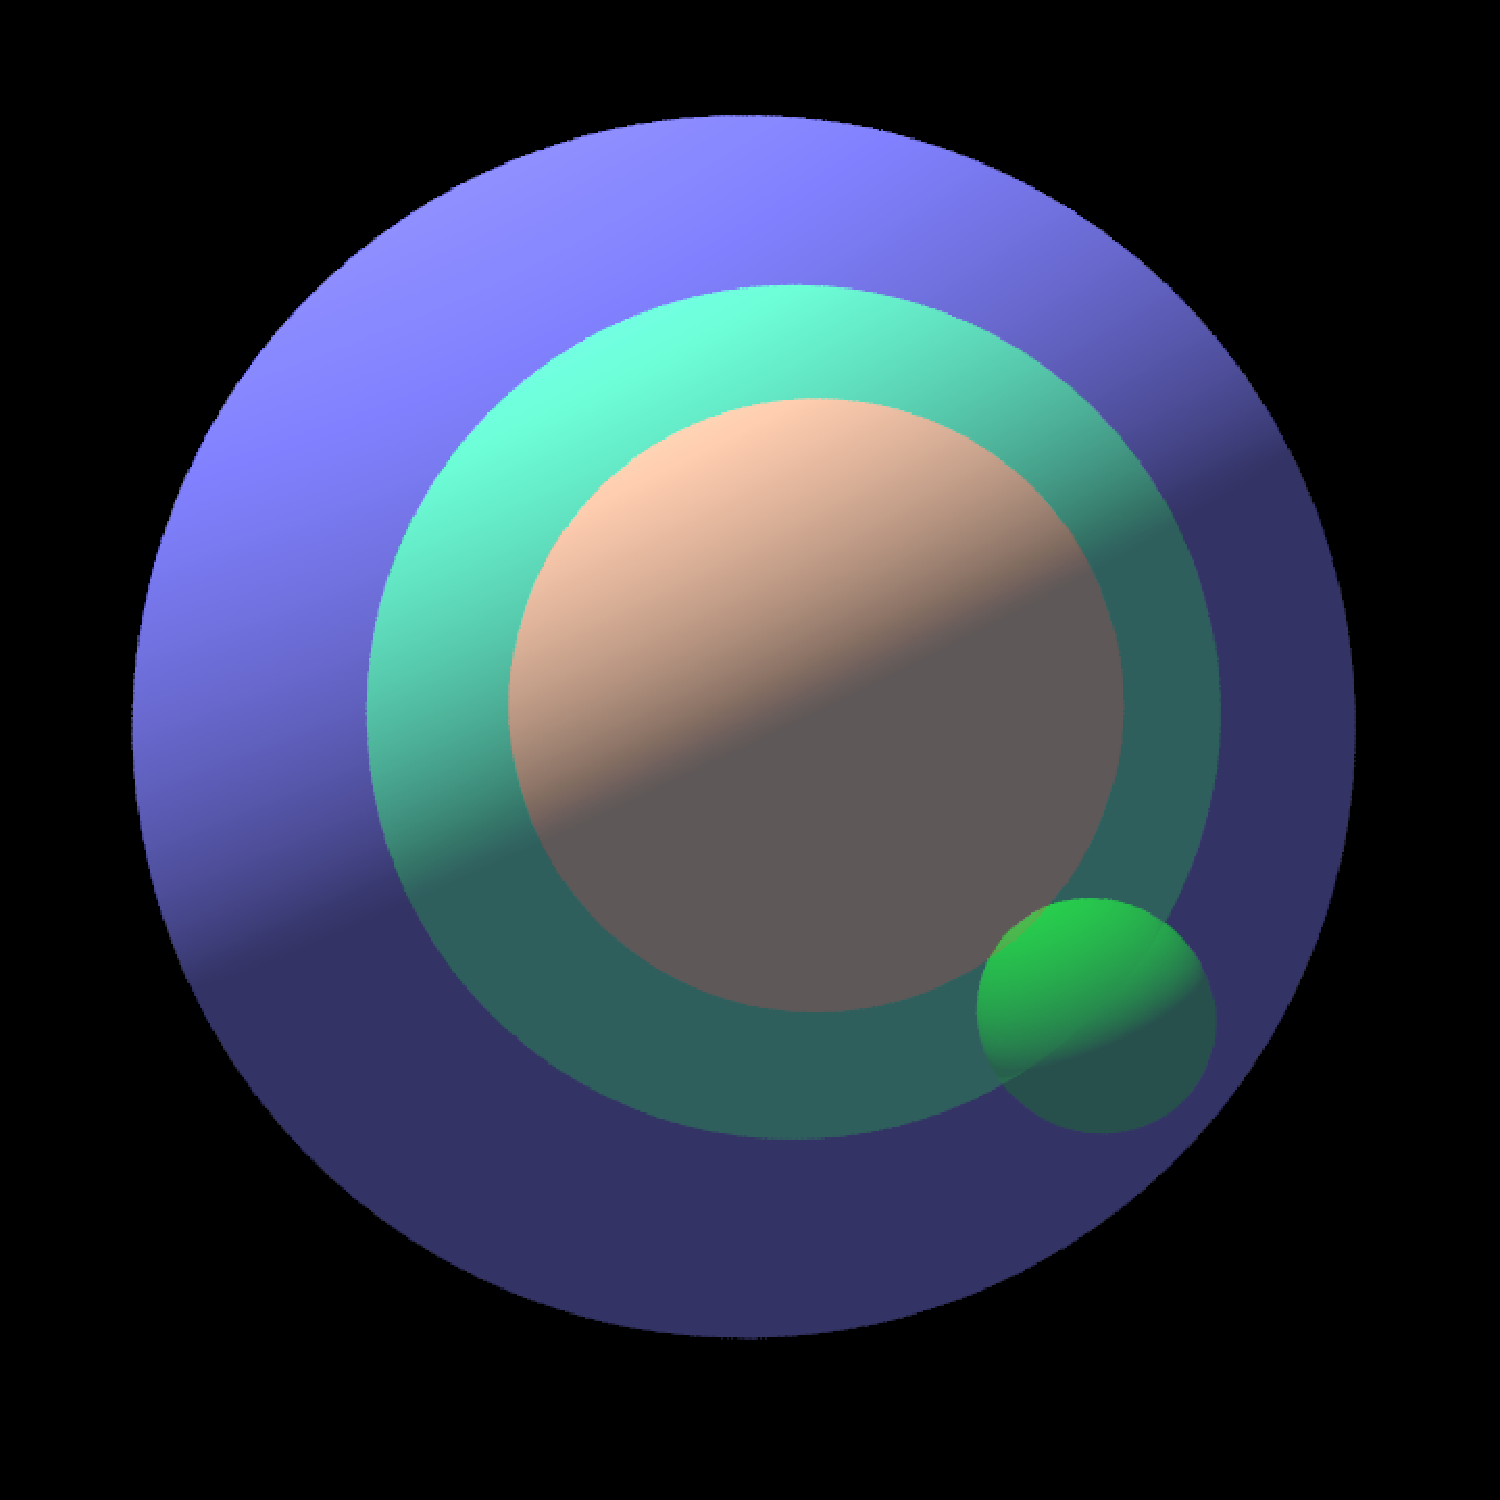
\includegraphics[width=1.4in, height=1.4in, keepaspectratio]{./img/application/3dGen/loxoGenSimple.pdf}
   \subcaption{\textit{Generator}}
   \label{fig:loxoGen3d}
  \end{minipage}
  \hspace*{\fill}
  \begin{minipage}{0.25\hsize}
   \center
   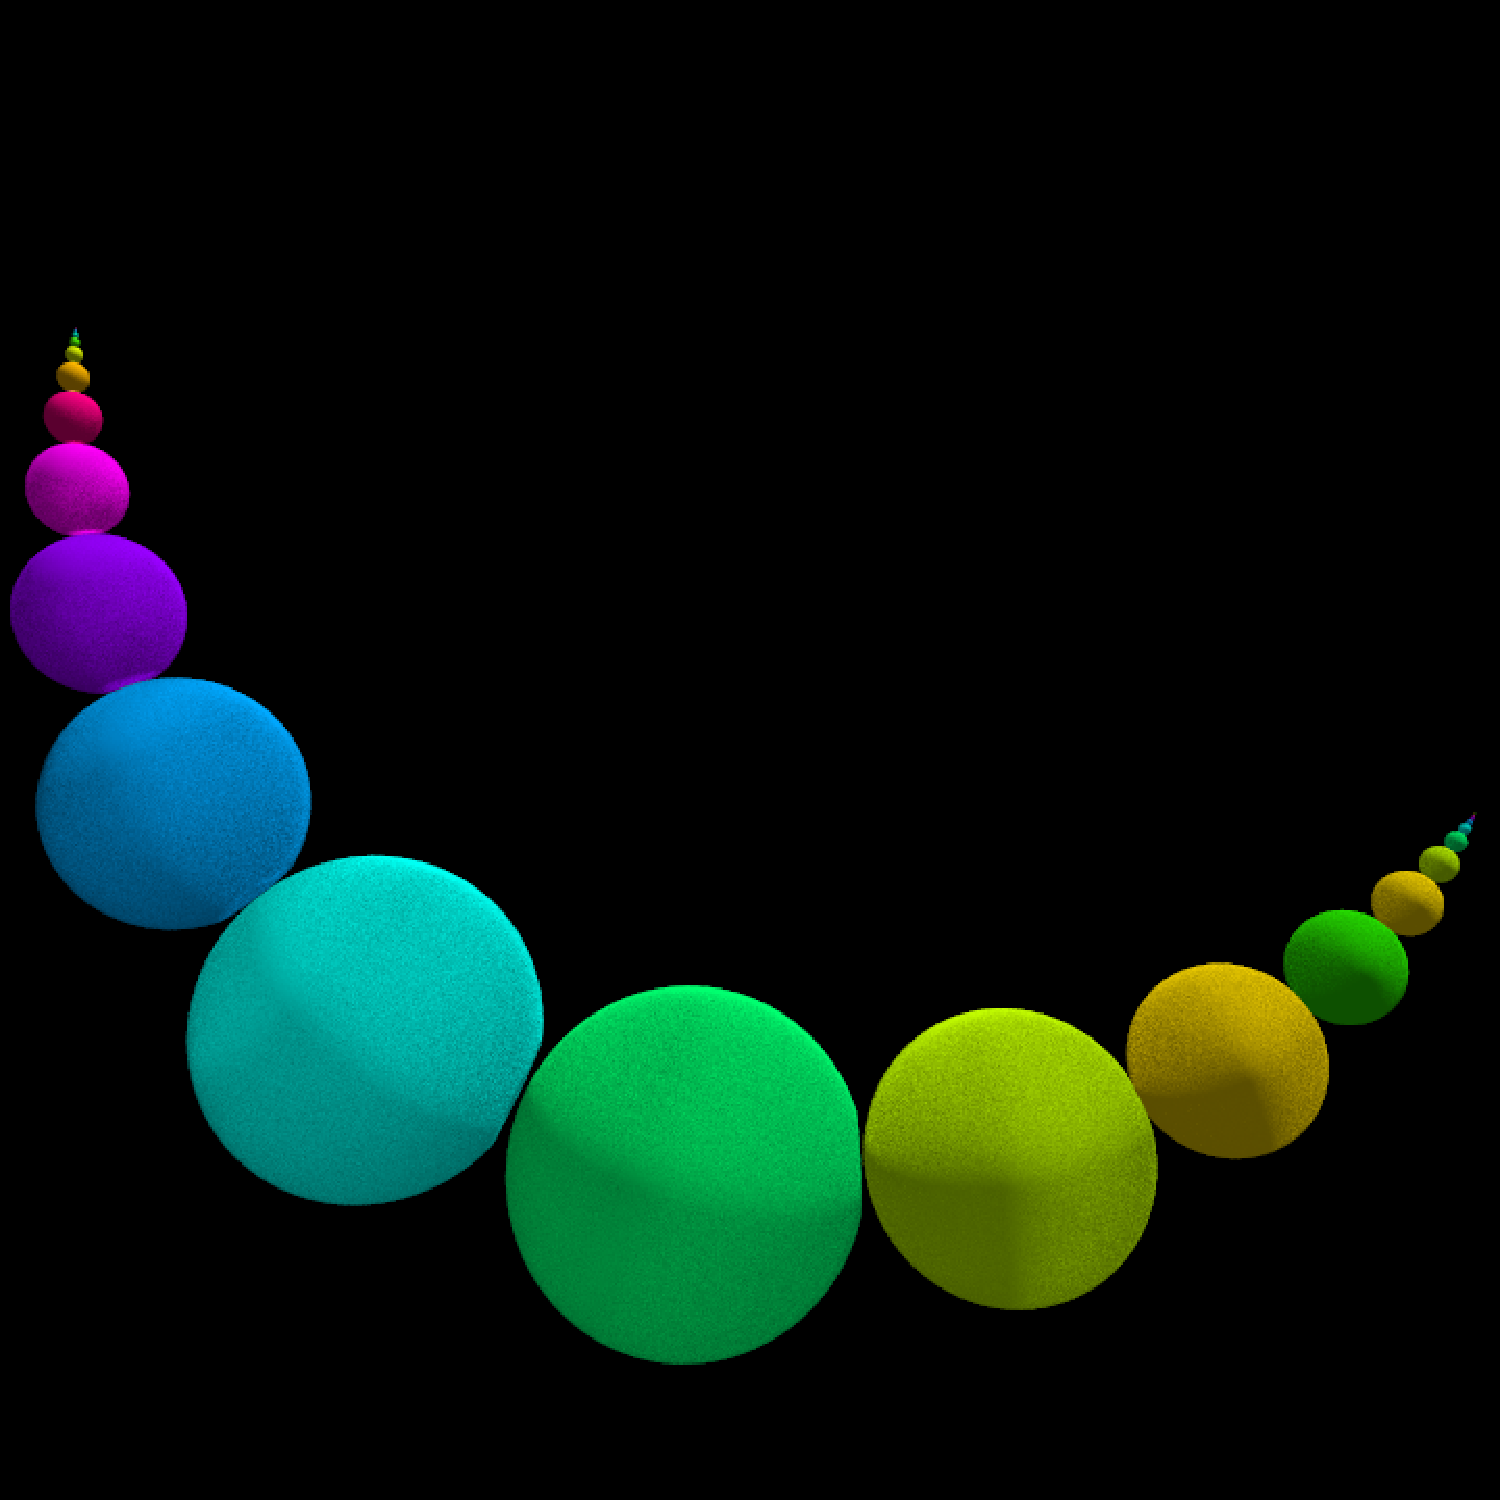
\includegraphics[width=1.4in, height=1.4in, keepaspectratio]{./img/application/3dGen/loxoOrbSimple.pdf}
   \subcaption{\textit{Orbit}}
   \label{fig:loxoOrb3d}
  \end{minipage}
  \hspace*{\fill}
 \caption{\textit{Hyperbolic generator and a base sphere.}}
  \label{fig:loxo3d}
 \end{minipage}
 \hspace*{\fill}
 \begin{minipage}{0.5\hsize}
  \begin{minipage}{0.25\hsize}
   \center
   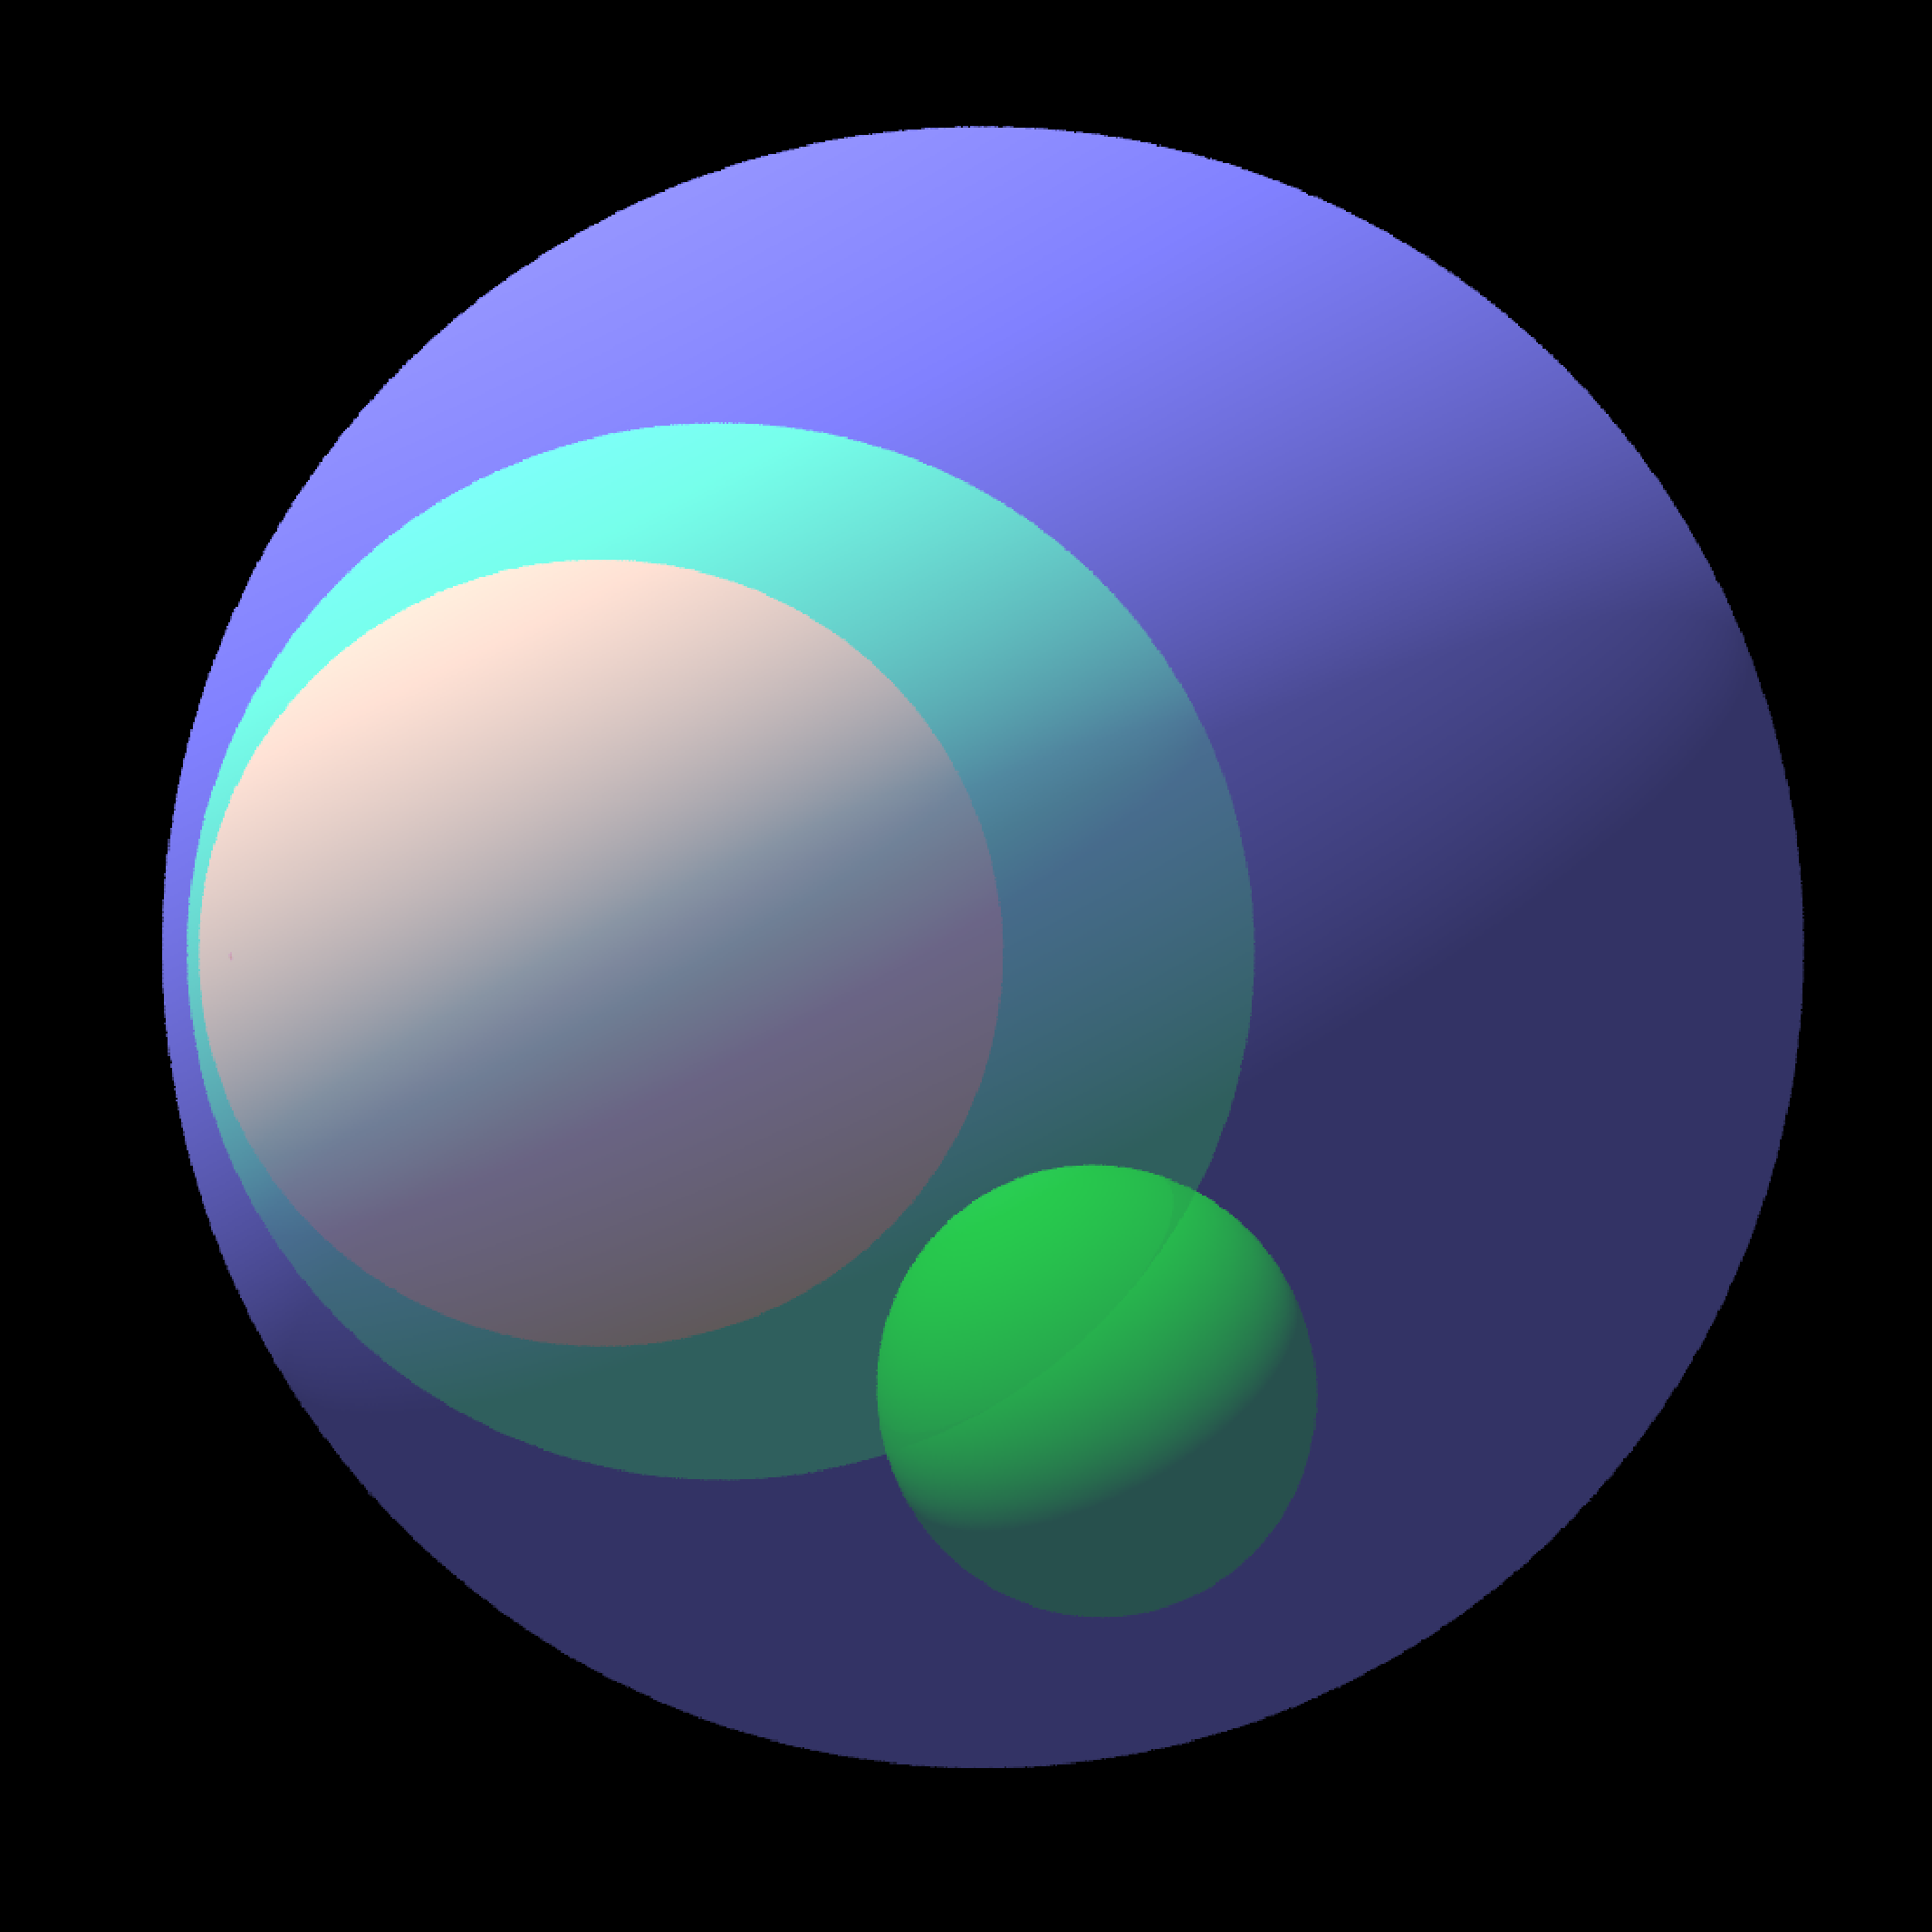
\includegraphics[width=1.4in, height=1.4in, keepaspectratio]{./img/application/3dGen/parabolicOneGen.pdf}
   \subcaption{\textit{Generator}}
   \label{fig:parabolic3dGen}
  \end{minipage}
  \hspace*{\fill}
  \begin{minipage}{0.25\hsize}
   \center
   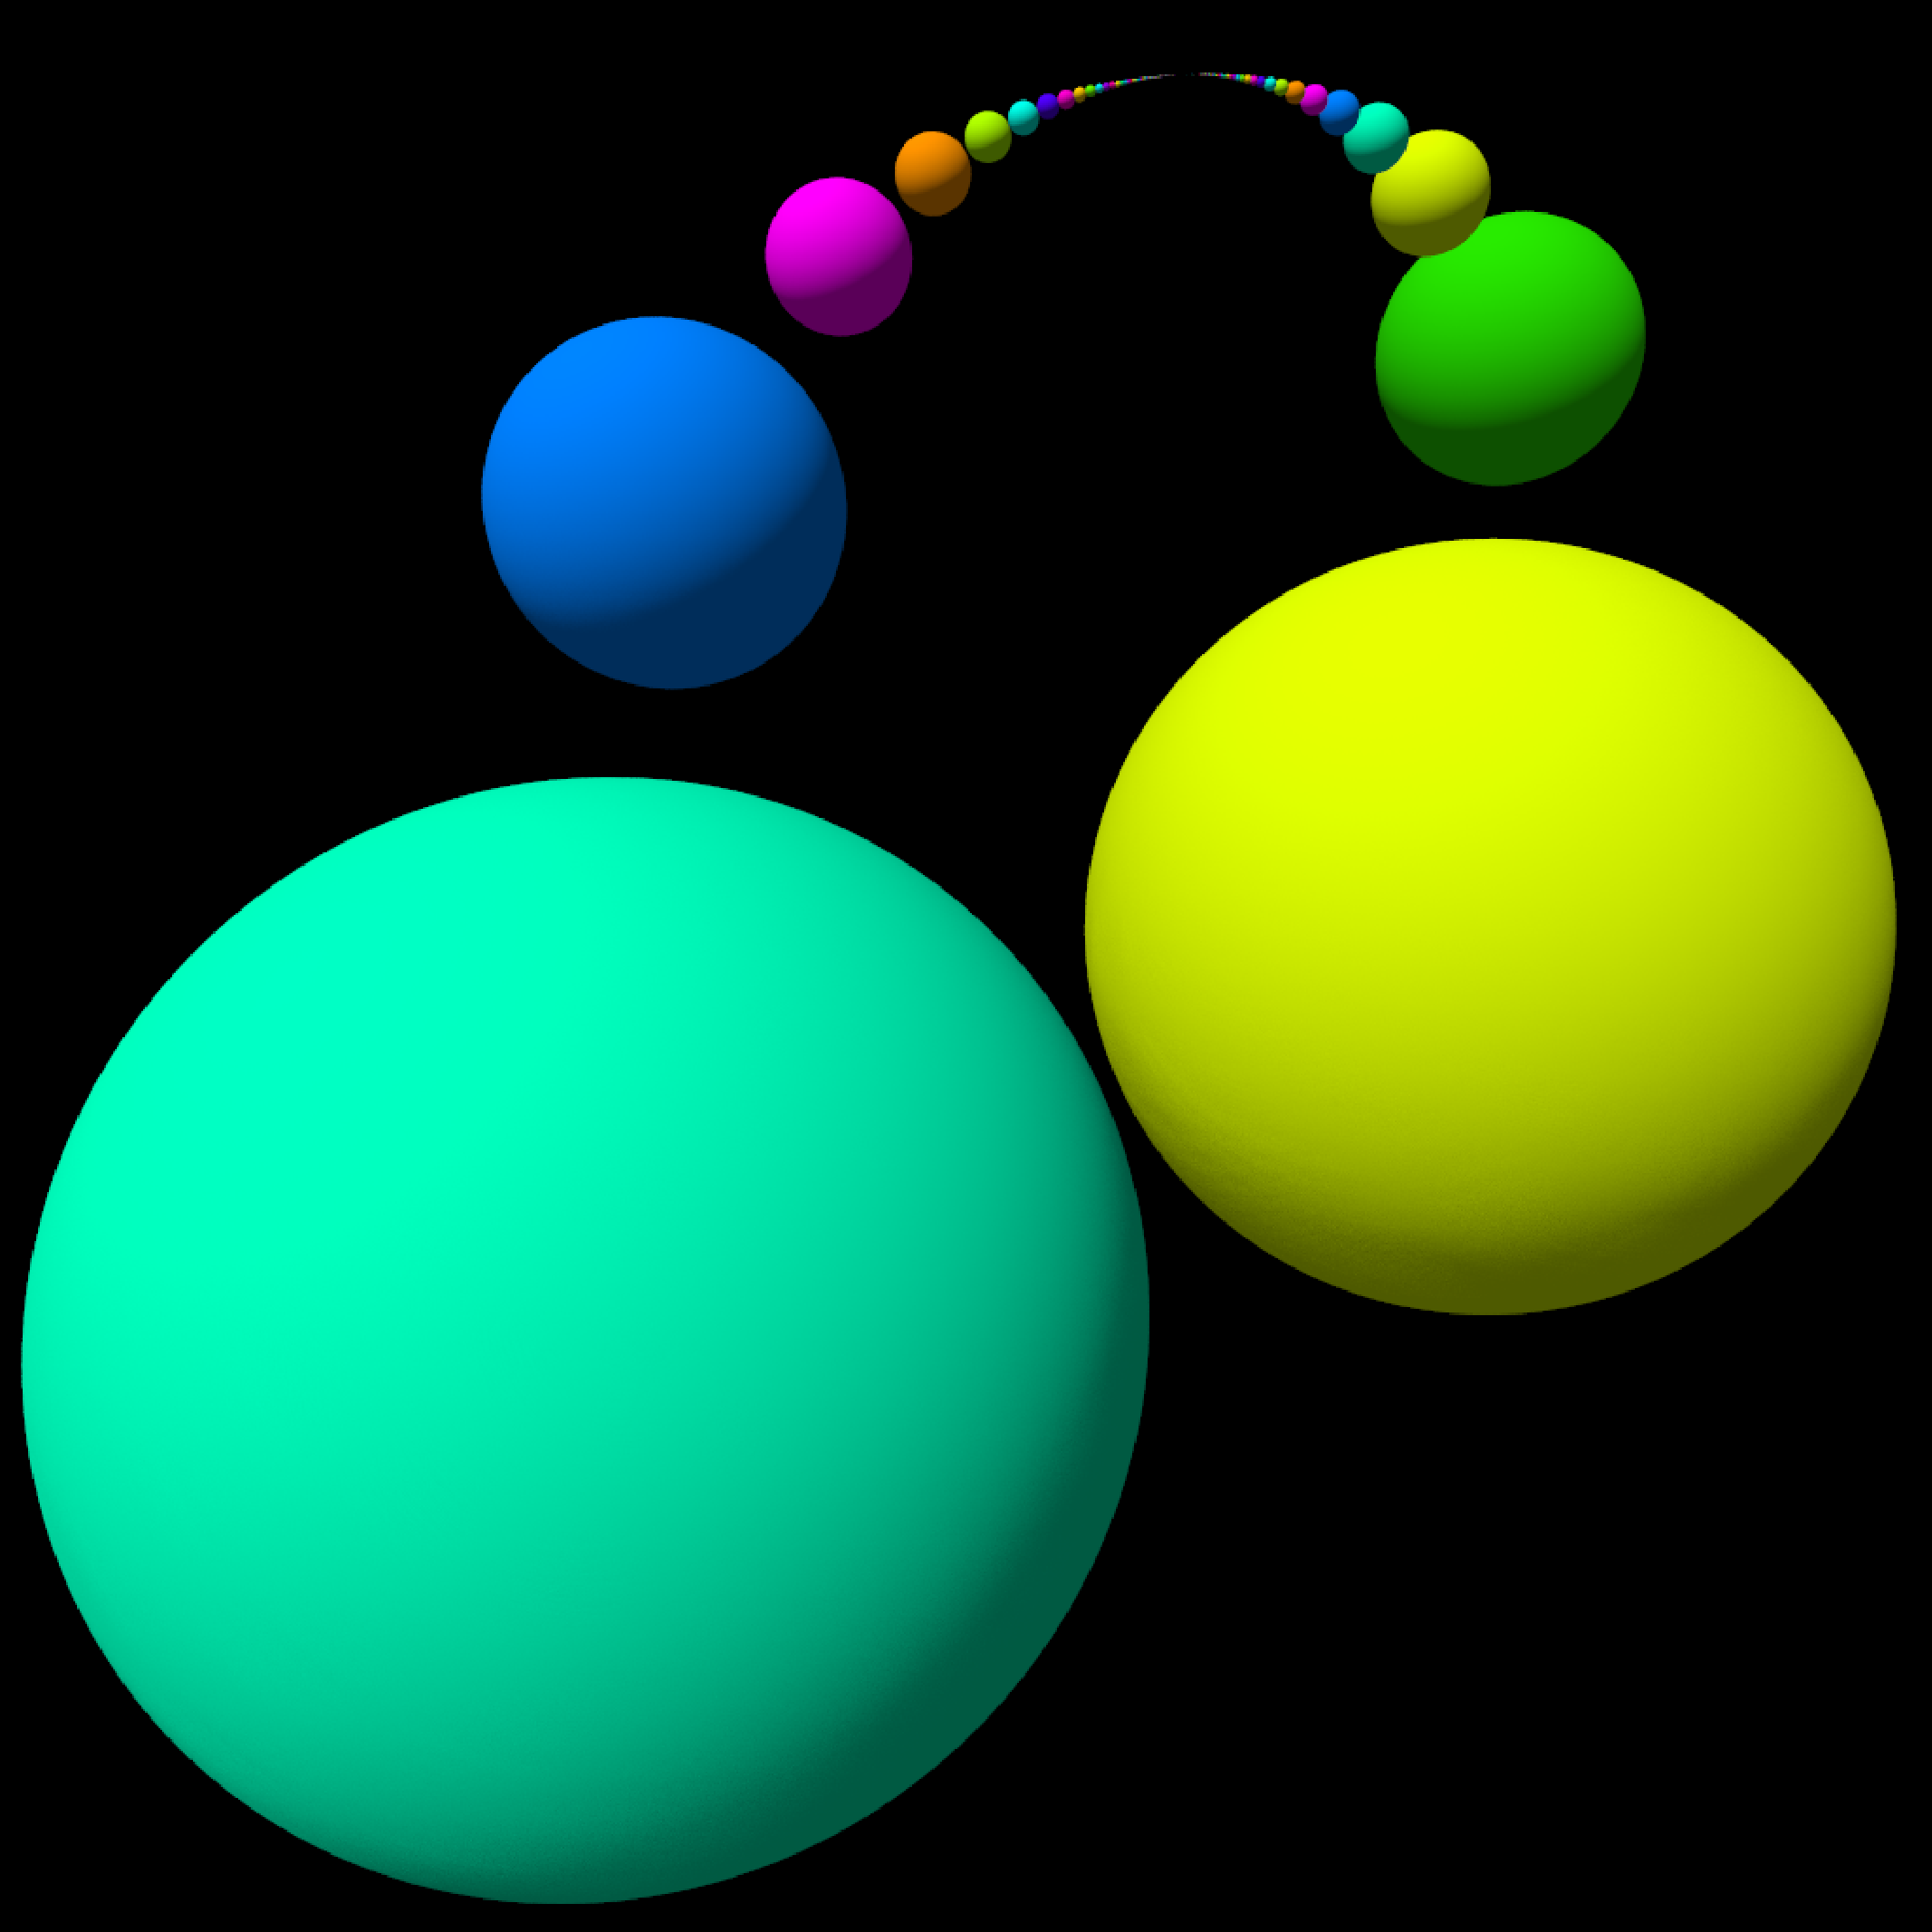
\includegraphics[width=1.4in, height=1.4in, keepaspectratio]{./img/application/3dGen/parabolicOneOrb.pdf}
  \subcaption{\textit{Orbit}}
   \label{fig:parabolic3dOrb}
  \end{minipage}
  \hspace*{\fill}
  \caption{\textit{Parabolic generator and a base sphere.}}
  \label{fig:parabolic3d}
 \end{minipage}
\end{figure}

\begin{figure}[htbp]
  \begin{minipage}{0.5\hsize}
   \center
   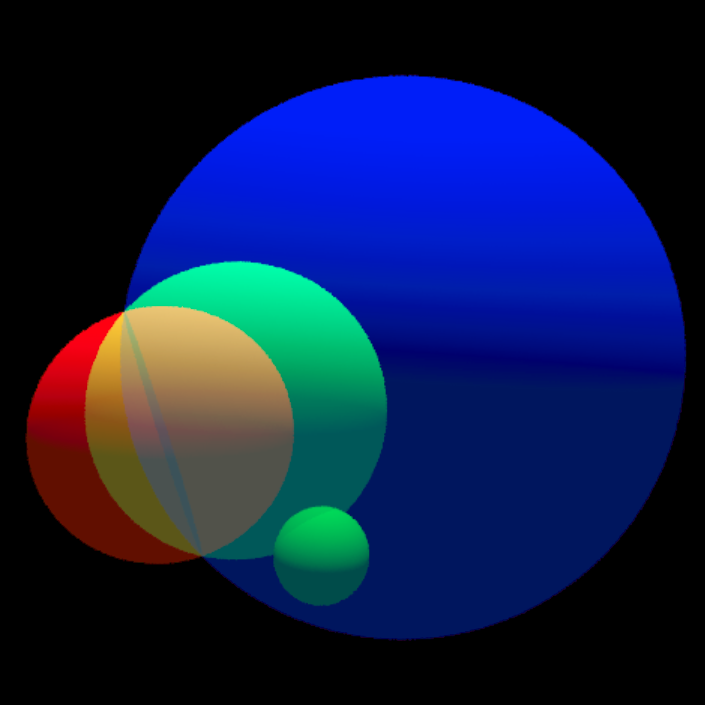
\includegraphics[ height=1.4in, keepaspectratio]{./img/application/3dGen/elliptic3Gen.png}
   \subcaption{\textit{Generator}}
   \label{fig:elliptic3dGen}
  \end{minipage}
 \hspace*{\fill}
  \begin{minipage}{0.5\hsize}
   \center
   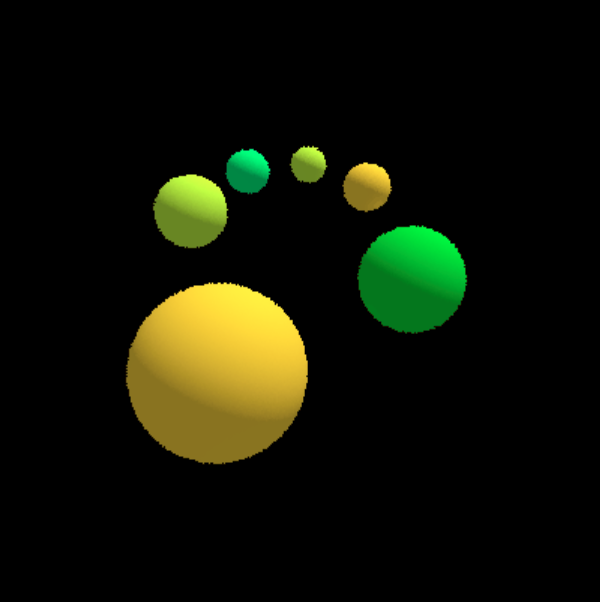
\includegraphics[ height=1.4in, keepaspectratio]{./img/application/3dGen/elliptic3Orb.png}
   \subcaption{\textit{Orbit}}
   \label{fig:elliptic3dOrb}
  \end{minipage}
 \hspace*{\fill}
  \caption{\textit{Elliptic generator and a base sphere.}}
  \label{fig:elliptic3d}
\end{figure}


\begin{figure}[h!tbp]
 \begin{minipage}[t]{0.5\hsize}
  \begin{minipage}[t]{0.25\hsize}
   \center
   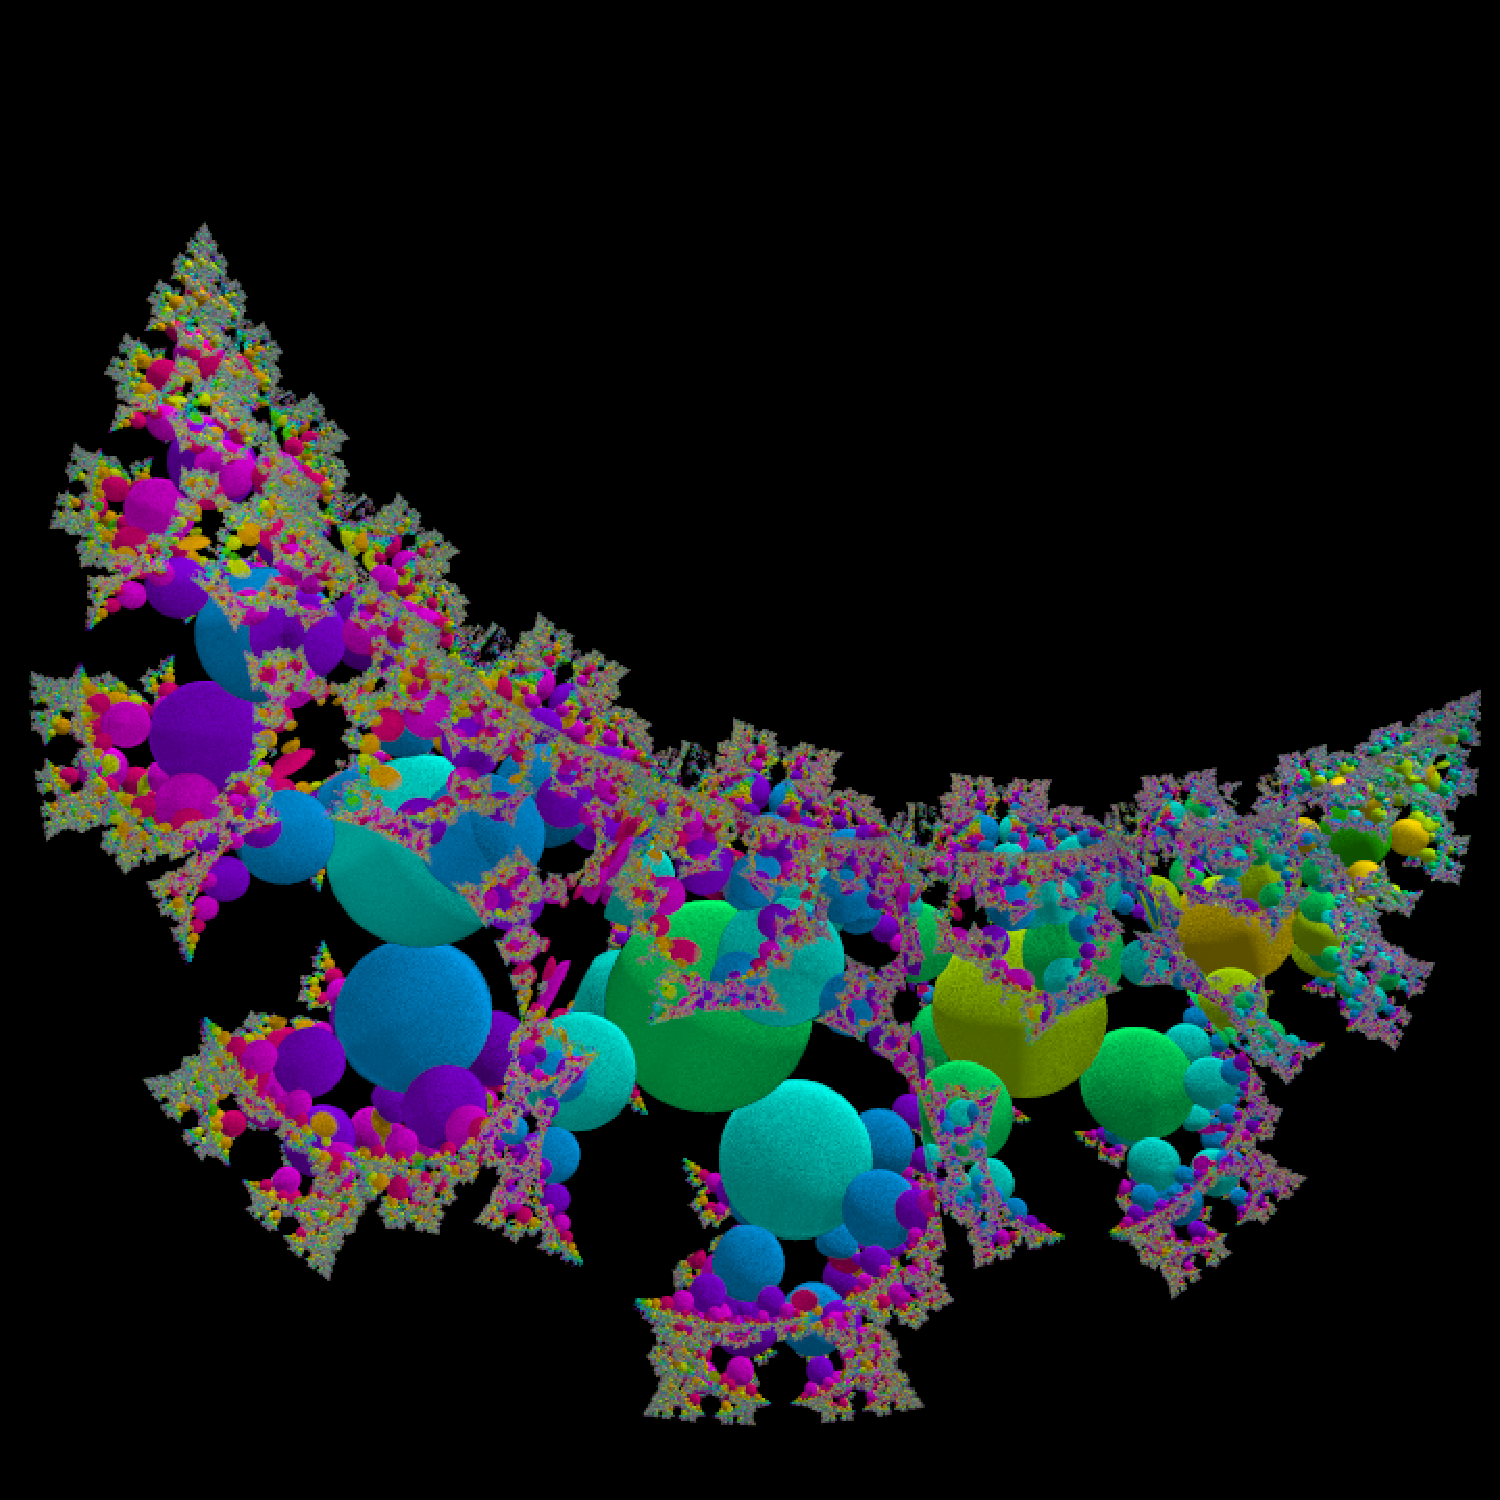
\includegraphics[width=1.4in, height=1.4in, keepaspectratio]{./img/application/3dGen/loxoOrbSch.pdf}
   \subcaption{\textit{Hyperbolic}}
  \end{minipage}
  \hspace*{\fill}
  \begin{minipage}[t]{0.25\hsize}
   \center
   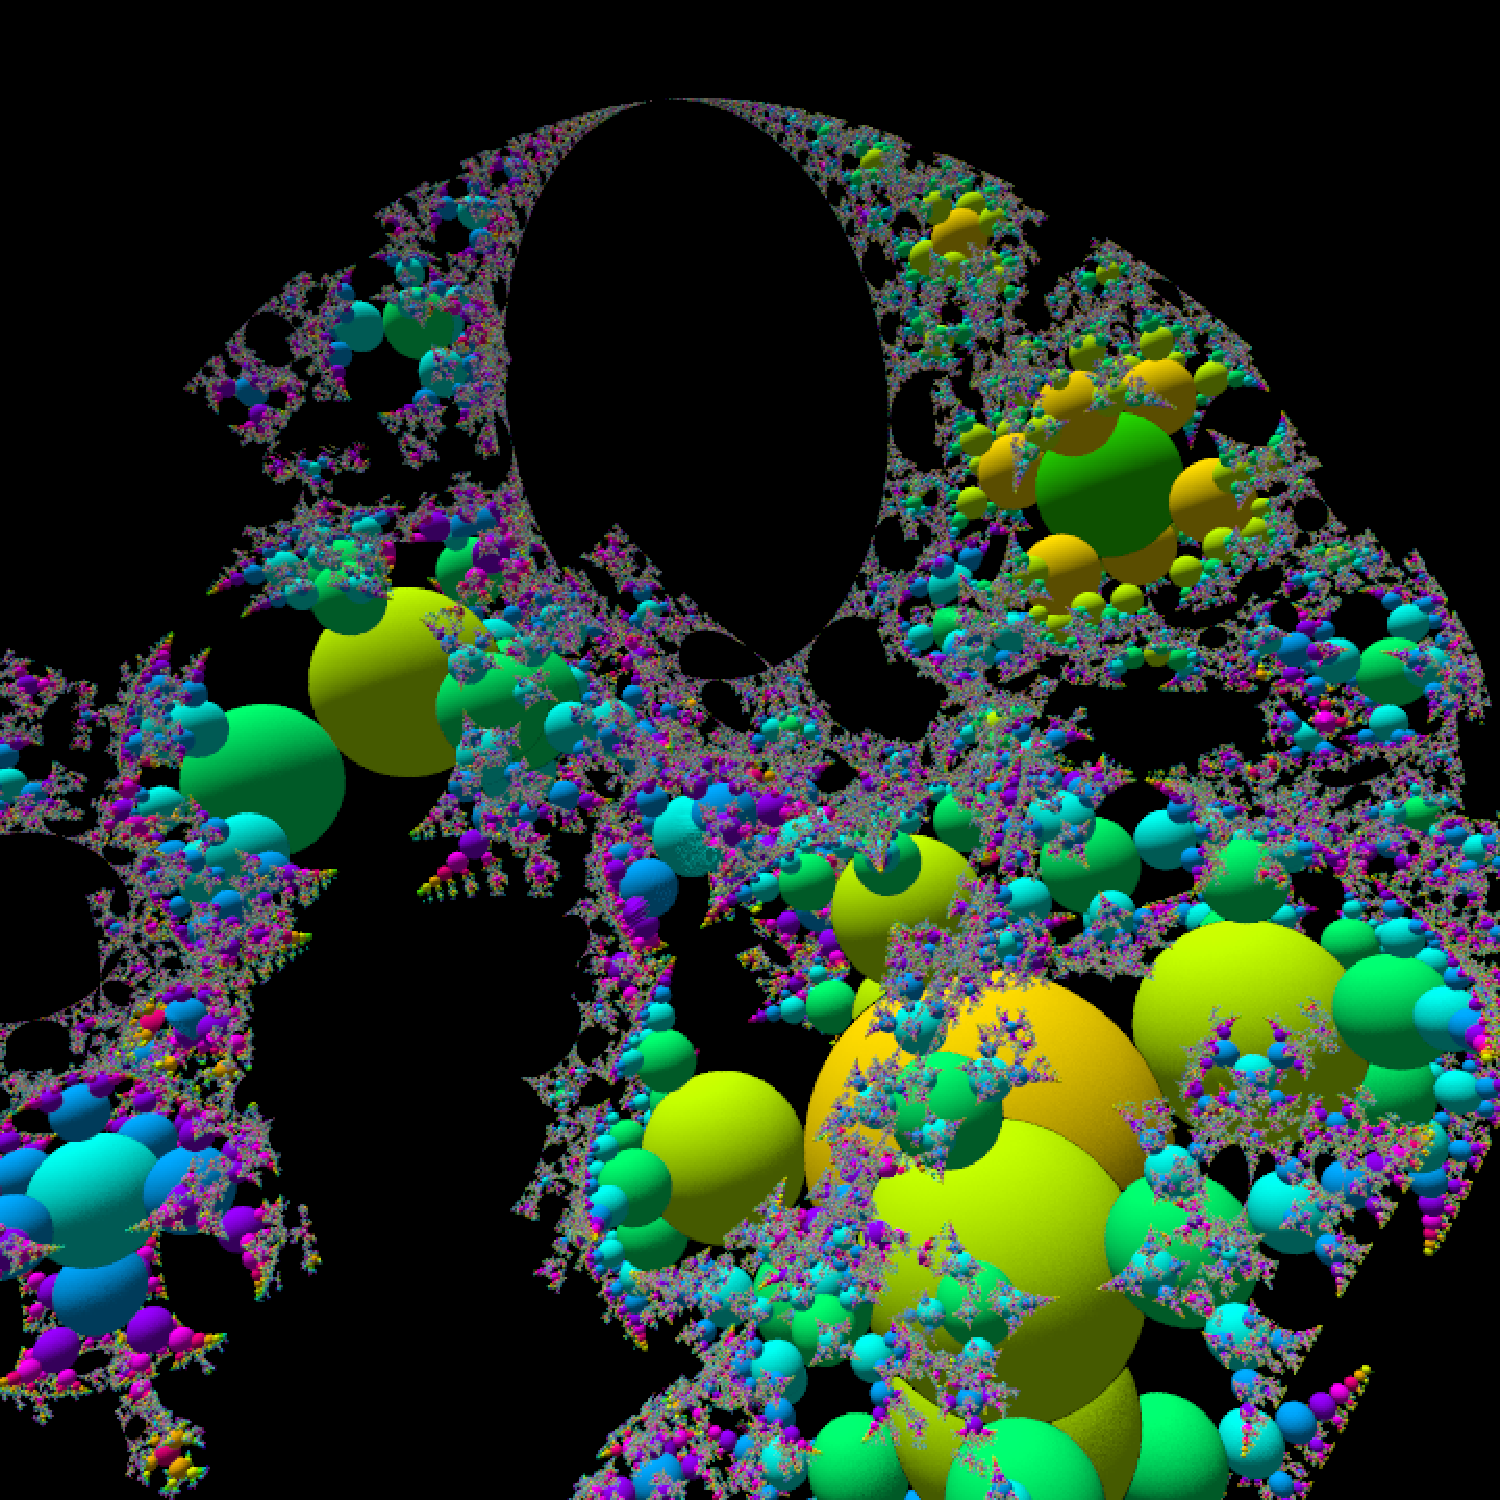
\includegraphics[width=1.4in, height=1.4in, keepaspectratio]{./img/application/3dGen/parabolicOrb.pdf}
   \subcaption{\textit{Parabolic}}
  \end{minipage}
  \hspace*{\fill}
  \caption{\textit{The orbit generated by a composition \\of two spheres and six Schottky
  spheres.}}
  \label{fig:complicated3d}
 \end{minipage}
 \hspace*{\fill}
 \begin{minipage}[t]{0.5\hsize}
  \begin{minipage}[t]{0.25\hsize}
   \center
   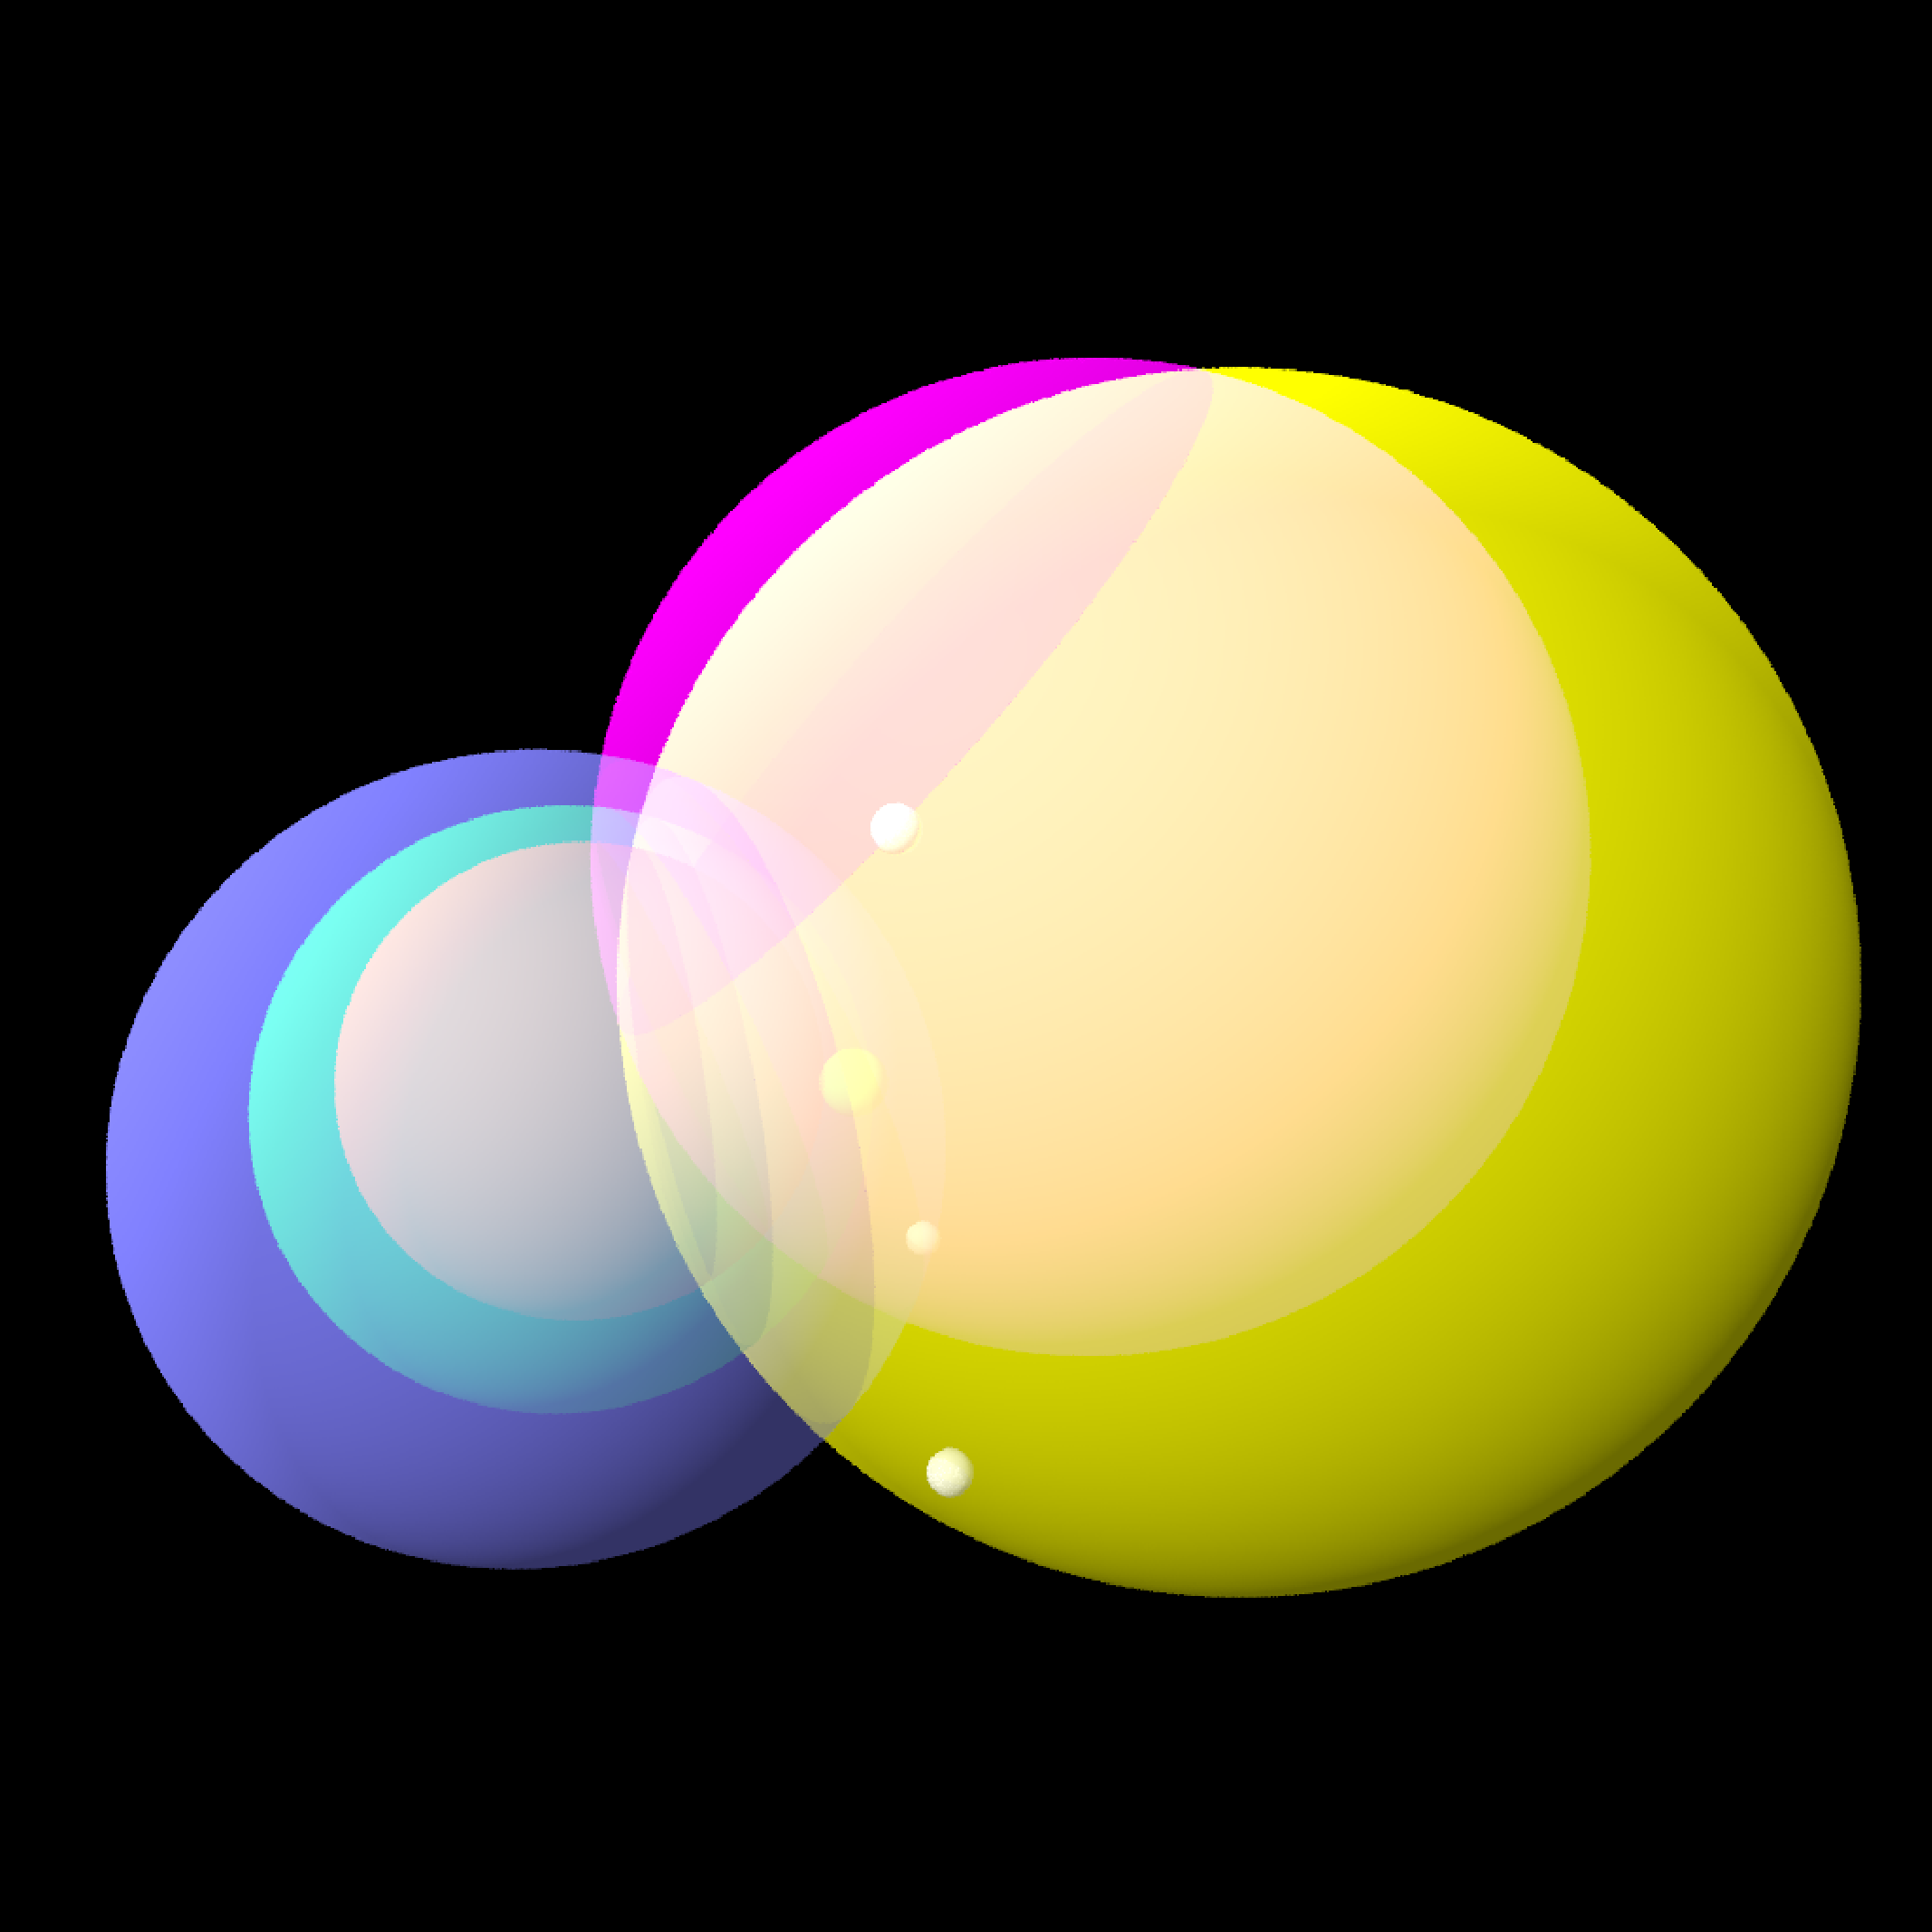
\includegraphics[width=1.4in, height=1.4in, keepaspectratio]{./img/application/3dGen/compLoxoOneGen.pdf}
   \subcaption{\textit{Generator}}
   \label{fig:compLoxoGen}
  \end{minipage}
 \hspace*{\fill}
  \begin{minipage}[t]{0.25\hsize}
   \center
   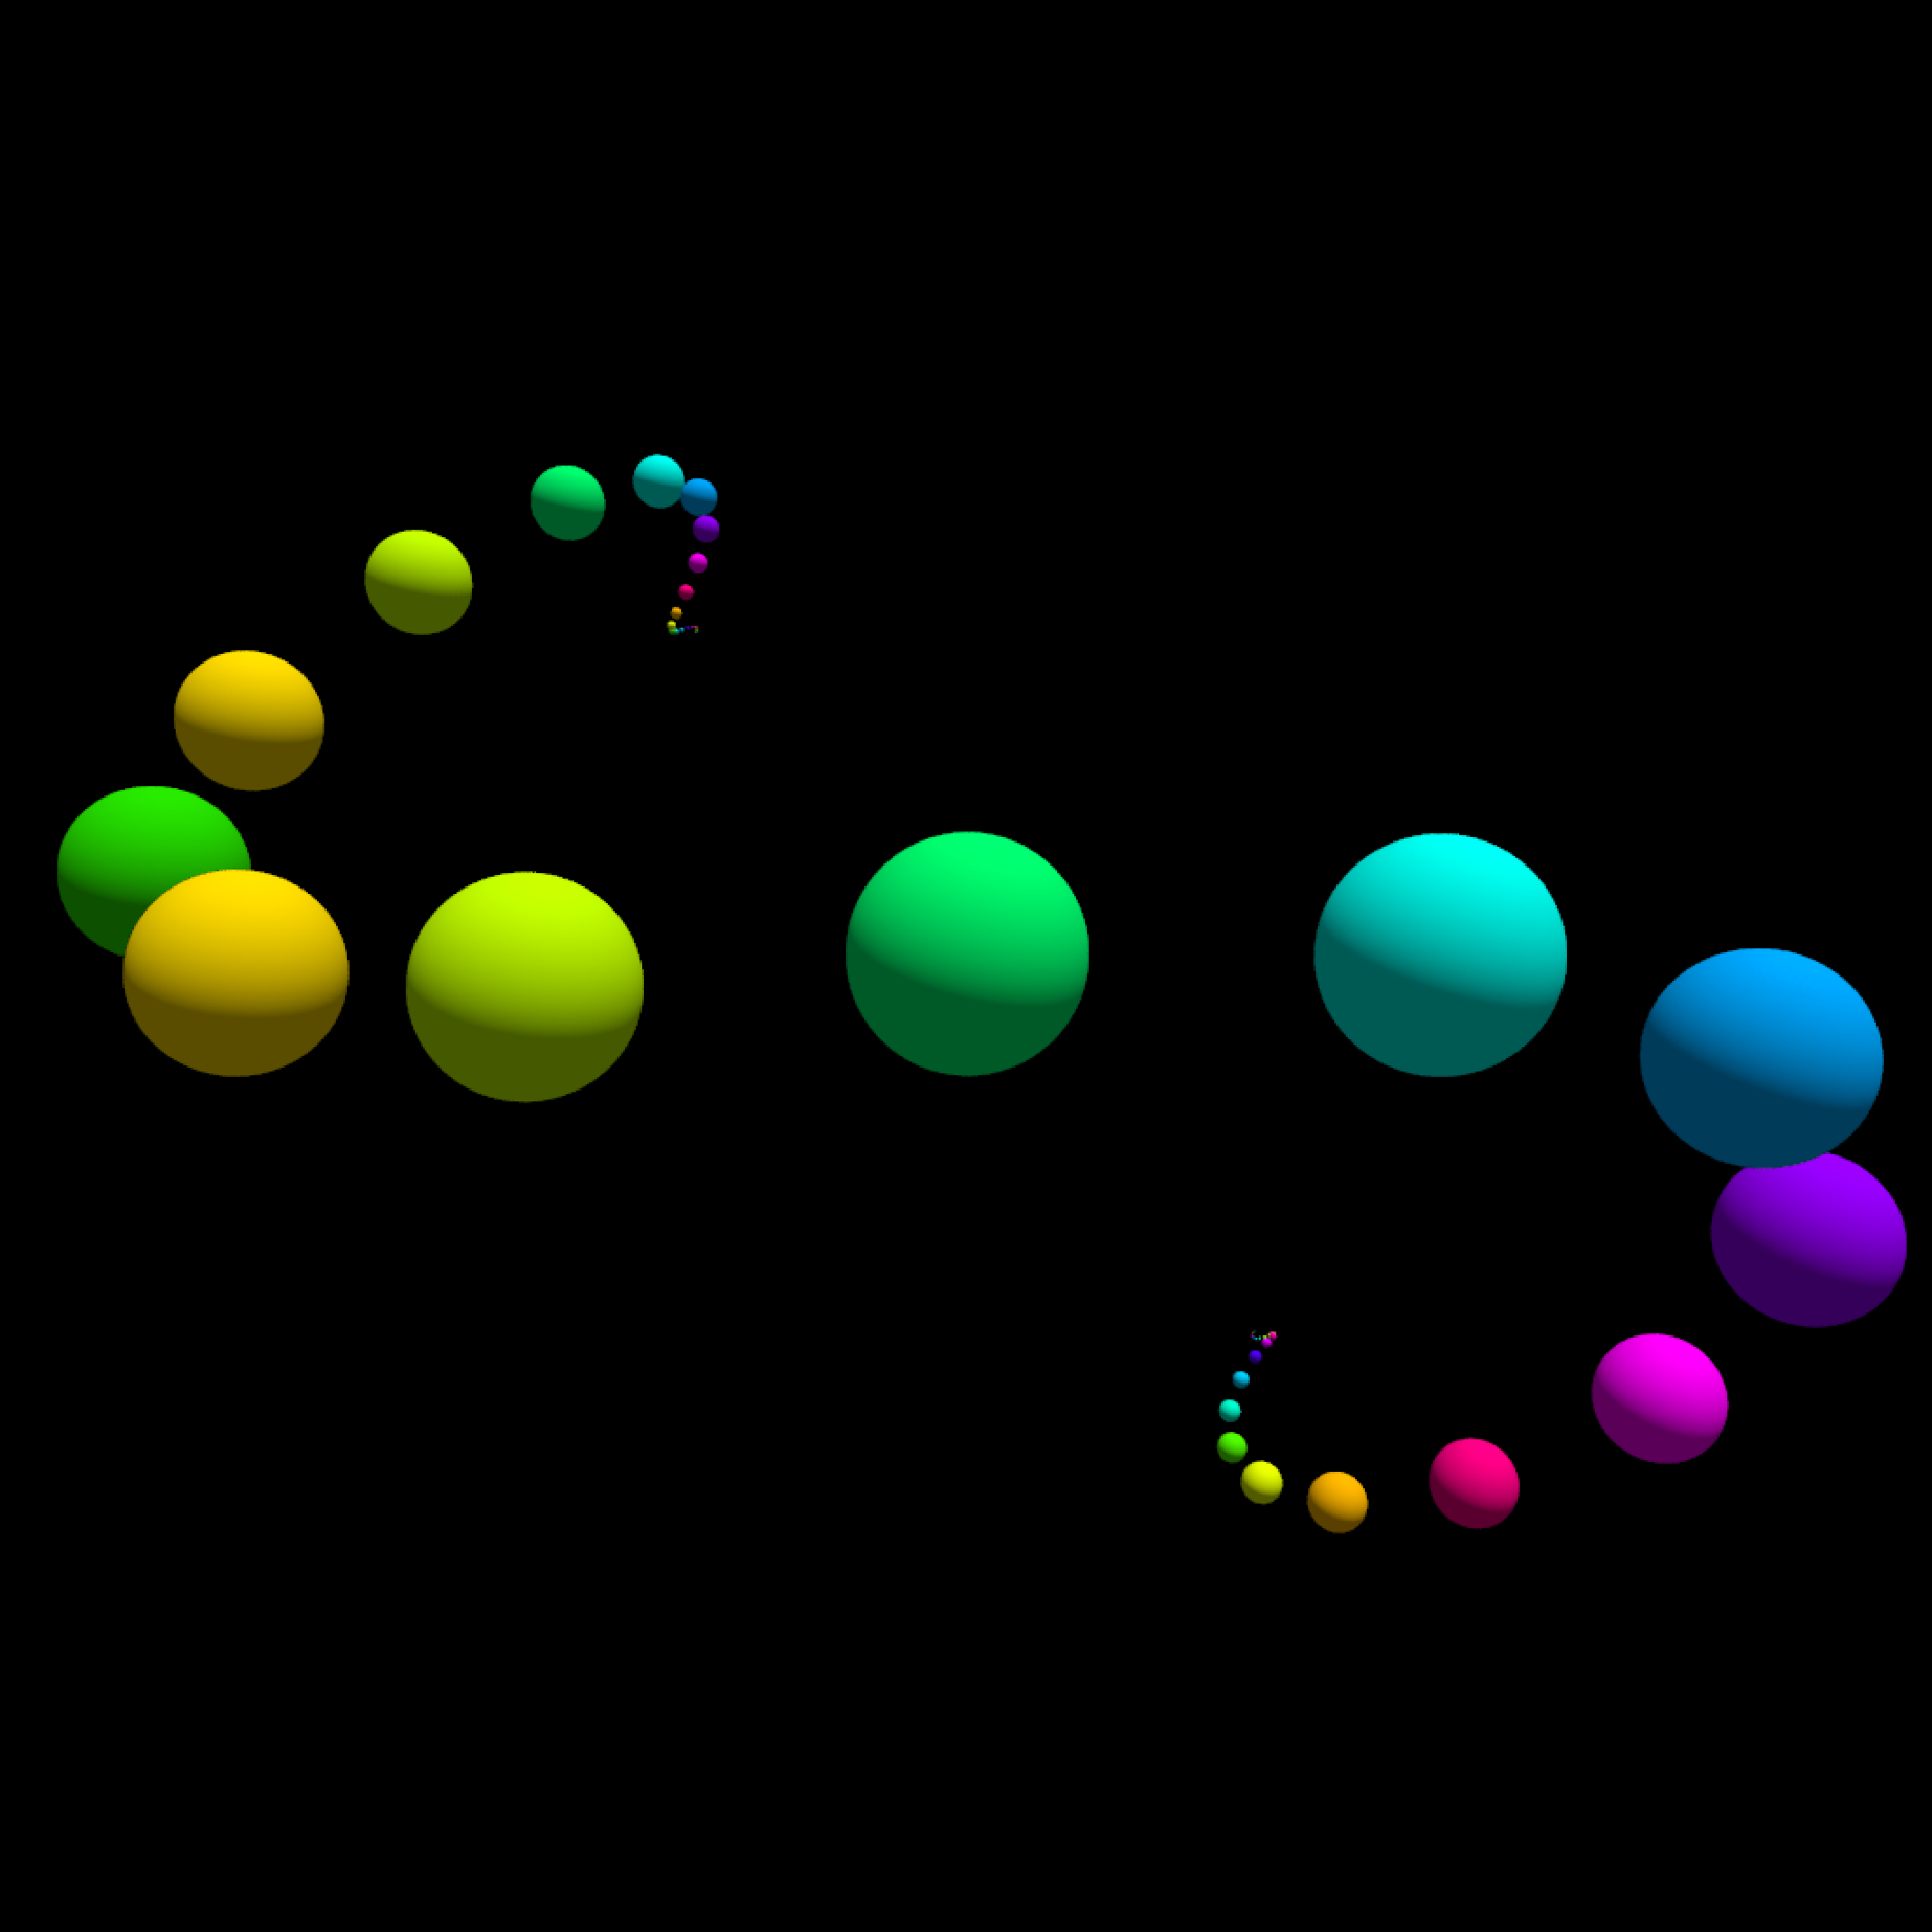
\includegraphics[width=1.4in, height=1.4in, keepaspectratio]{./img/application/3dGen/compLoxoOneOrb.pdf}
   \subcaption{\textit{Orbit}}
   \label{fig:compLoxoOrb}
  \end{minipage}
  \hspace*{\fill}
  \caption{\textit{Compound loxodromic generator and a base sphere.}}
  \label{fig:compLoxo}
 \end{minipage}
\end{figure}

\noindent\textbf{Inversion in a Sphere with Infinite Radius.}
An inversion in a sphere with infinite radius is represented by
a reflection through a plane.
See Figure \ref{fig:infSphere}\subref{fig:infSphereGen}.
There are four white inversion spheres, one green base sphere,
and one blue plate.
The blue plate is a part of a sphere with infinite radius.
The orbit of the group is shown in Figure
\ref{fig:infSphere}\subref{fig:infSphereOrb}.
The resulting orbit has reflection symmetry.

\noindent\textbf{Parallel
Translation\footnote{\url{https://www.shadertoy.com/view/lsjyzK}}.}
A composition of inversions in two parallel planes represents a parallel
translation along a normal vector of the planes.
See Figure \ref{fig:translation3d}.
This is a parabolic transformation.
Moreover, in three-dimension, we can add a twist to the orbit.
See Figure \ref{fig:compParabolic}.
The orbit is rotated around the normal vector of the planes for every
translation.
This operation is possible in three-dimensional space because we have gained a degree
of freedom over two-dimensional space.
The transformations yielding twisted orbits are called \textit{compound
parabolic} transformations.

\noindent\textbf{Rotation.}
A composition of reflections through two crossing planes generates a rotation.
The axis of rotation is the intersection line of two planes.
The generators and the orbit are shown in Figure \ref{fig:rotation3d}.

\noindent\textbf{Composition of Two
Spheres\footnote{\url{https://www.shadertoy.com/view/ldByDW}}.}
We compose generators using two spheres.
See Figure \ref{fig:loxo3d}\subref{fig:loxoGen3d}.
We call the light red sphere $S1$, the light green sphere $S2$, and the blue
sphere $S1'$.
The map $G$ is as follows.
\begin{align*}
G =
\begin{cases}
 I_{S2} \circ I_{S1} & (\text{The point is inside of } S1) \\
 I_{S1} \circ I_{S2} & (\text{The point is outside of }S1')
\end{cases}
\end{align*}
While $S1$ and $S2$ have no intersection, the generator is hyperbolic
transformation.
The orbit of the base sphere is shown in Figure \ref{fig:loxo3d}\subref{fig:loxoOrb3d}.
When $S1$ and $S2$ come in contact with each other at one point as shown
in Figure \ref{fig:parabolic3d}\subref{fig:parabolic3dGen}, it becomes a
parabolic transformation.
The orbit of spheres touches at the fixed point.
It is shown in Figure \ref{fig:parabolic3d}\subref{fig:parabolic3dOrb}.

When $S1$ and $S2$ are crossing as in Figure \ref{fig:elliptic3d},
the generator becomes an elliptic transformation.
The orbit is as shown in Figure \ref{fig:elliptic3d}\subref{fig:elliptic3dOrb}.
Similarly to two-dimensional ones, the crossing angle of $S1$ and $S2$
should be rational angles;
otherwise the orbit of the spheres will overlap each other.

Also, Figure \ref{fig:complicated3d} shows the example of the more
complicated orbit of spheres generated by adding six inversion spheres to
the group shown in Figure \ref{fig:loxo3d} and Figure \ref{fig:parabolic3d}.

\noindent\textbf{Compound
Loxodromic\footnote{\url{https://www.shadertoy.com/view/MdjyRV}}.}
Finally, we add two spheres perpendicular to $S1$ and $S2$.
See Figure \ref{fig:compLoxo}\subref{fig:compLoxoGen}.
We call pink sphere $S3$ and yellow sphere $S4$, and there are three
user-defined control points $P$, $Q1$, and $Q2$.
$S3$ and $S4$ are determined by four points.
Let $P'$ and $P''$ be inversions of $P$ in $S1$ and $S2$.
The spheres and the map $G$ are as follows.
\begin{align*}
S3 = Sphere(P,~P',~P'',~Q1) \quad
S4 = Sphere(P,~P',~P'',~Q2) \\
G =
\begin{cases}
 (I_{S4} \circ I_{S3}) \circ (I_{S1} \circ I_{S2}) & (\text{The point is inside of } S1) \\
 (I_{S2} \circ I_{S1}) \circ (I_{S3} \circ I_{S4}) & (\text{The point is outside of }S1')\\
\end{cases}
\end{align*}
The composition of inversions in $S3$ and $S4$ represents rotation.
The twisted orbit shown in Figure
\ref{fig:compLoxo}\subref{fig:compLoxoOrb} is analogous to the loxodromic
transformations in two-dimension.
Therefore, we call this generator \textit{compound loxodromic}.


\begin{figure}[h!tbp]
 \begin{minipage}[t]{0.24\hsize}
  \begin{center}
   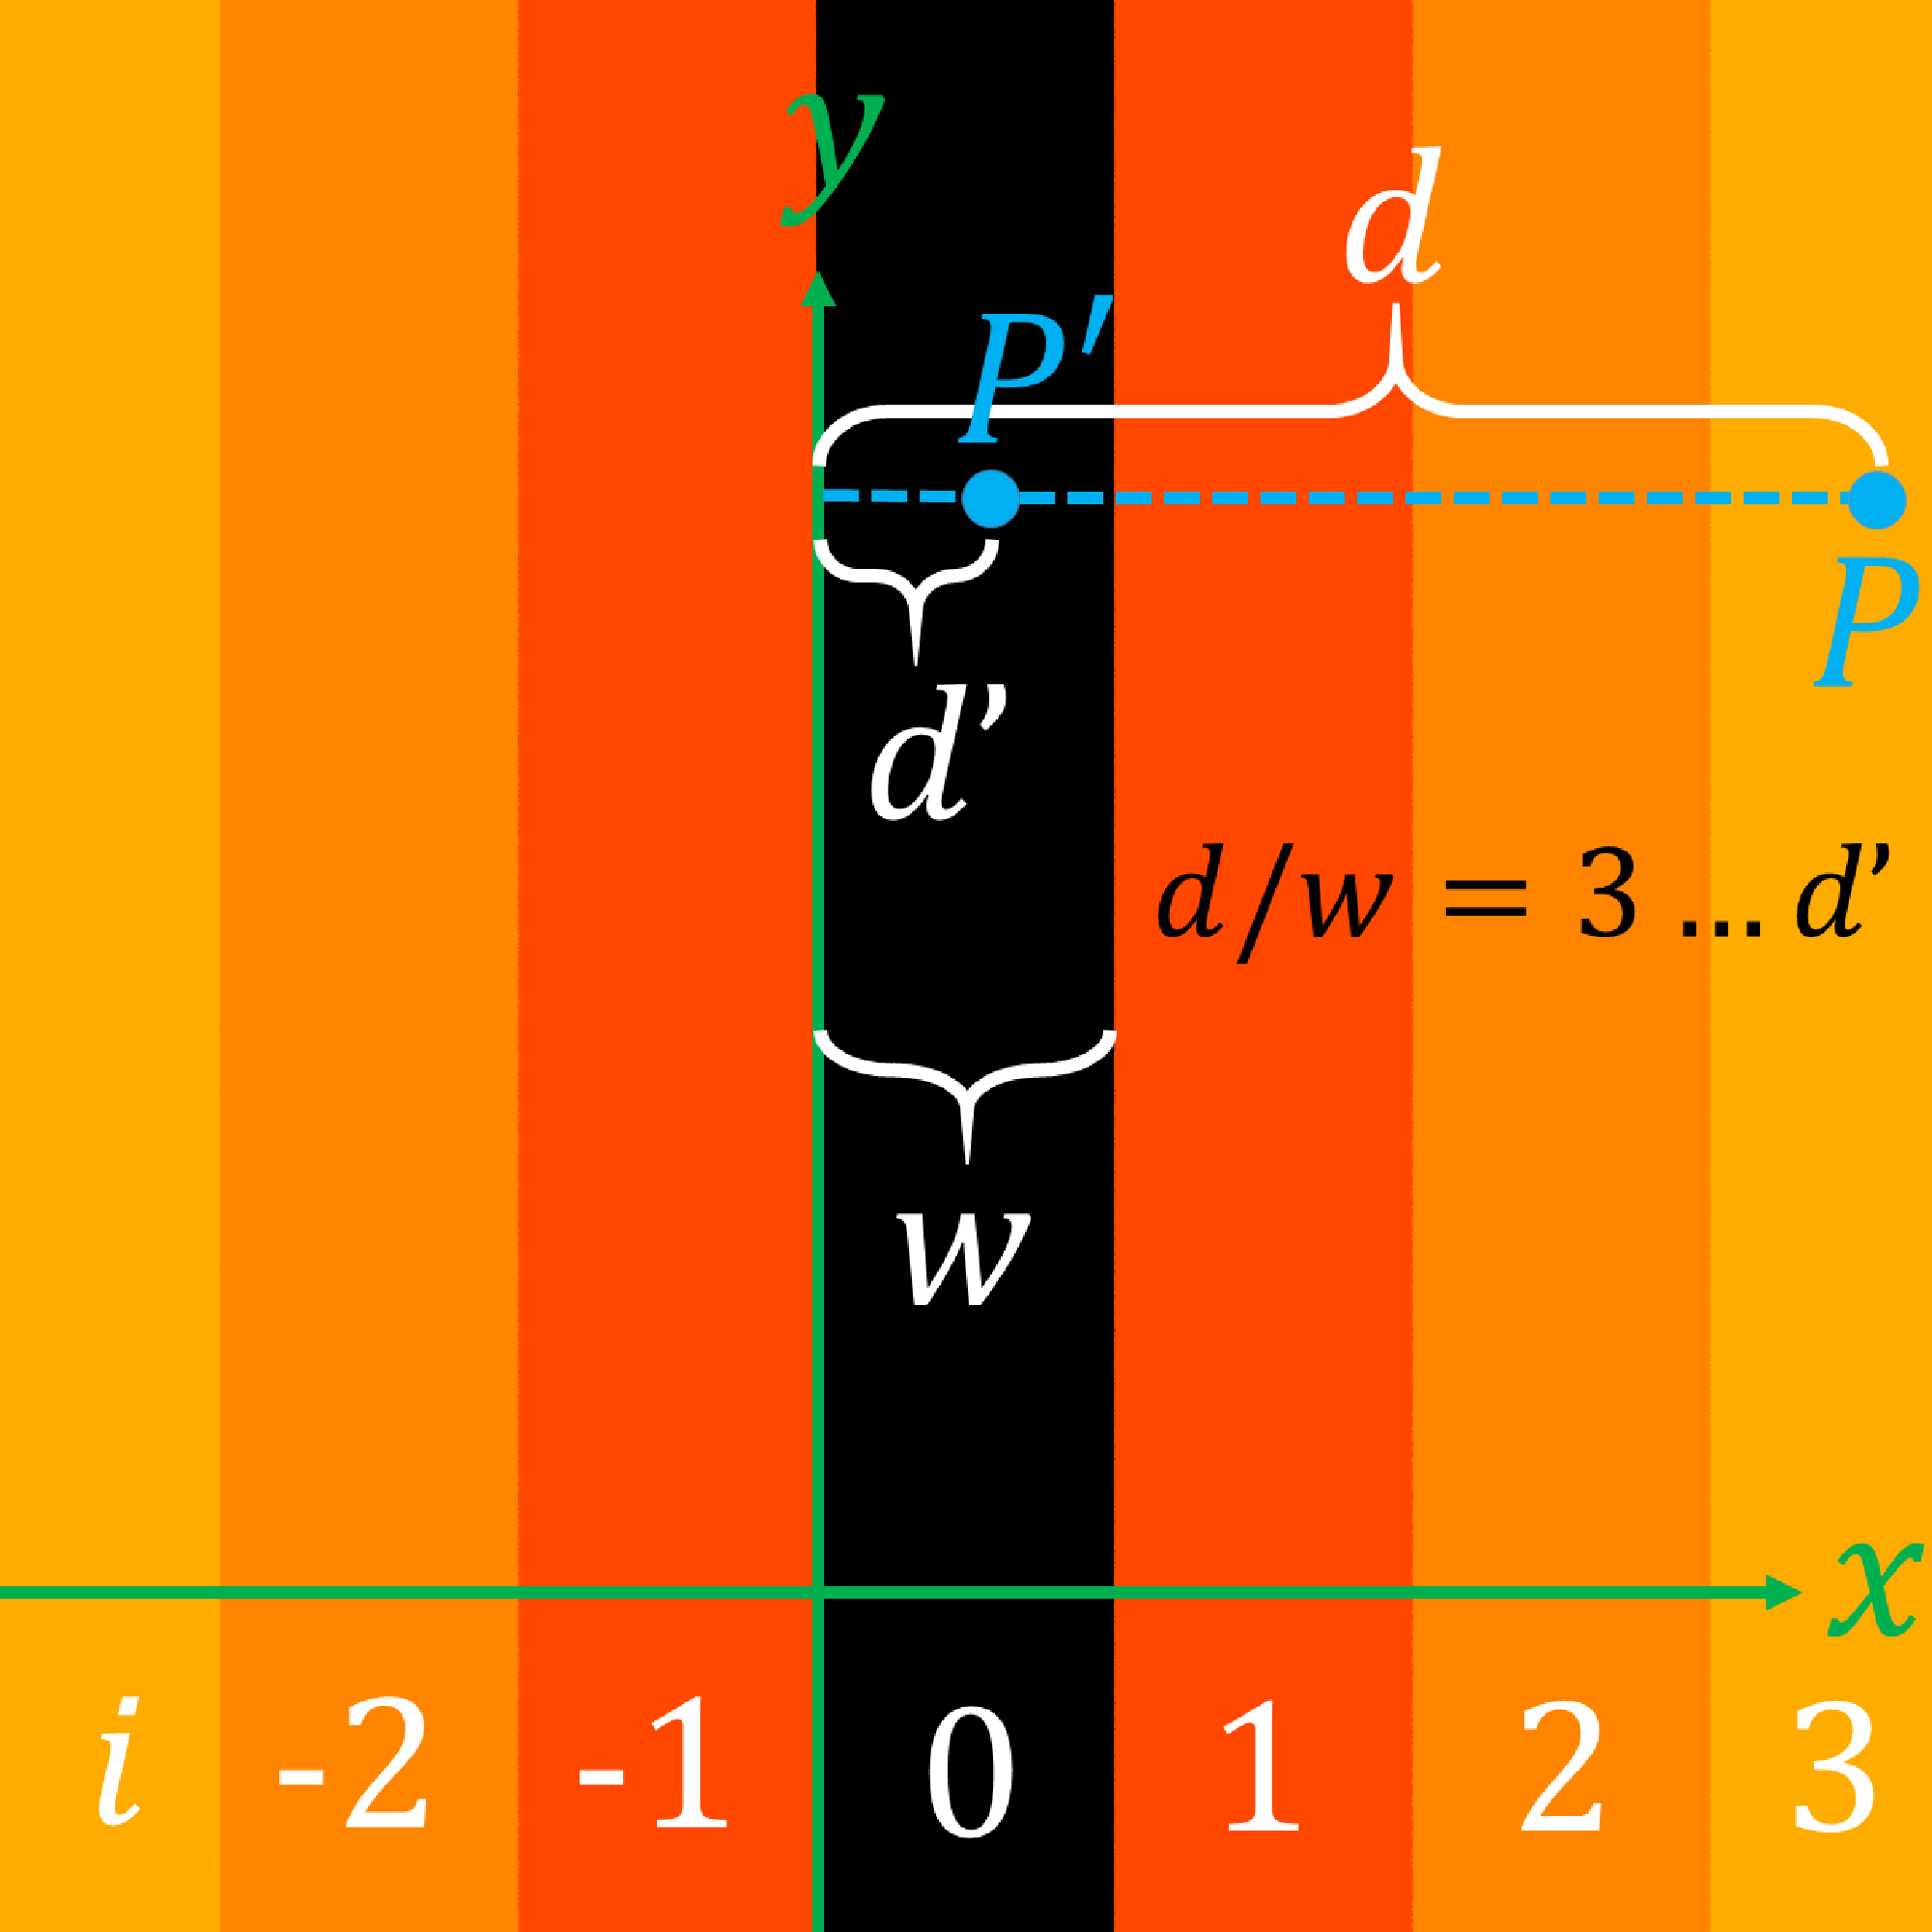
\includegraphics[width=1.5in, height=1.5in, keepaspectratio]{./img/application/optimization/translationMod.pdf}
  \end{center}
  \caption{\textit{Parallel translation.}}
  \label{fig:translationMod}
 \end{minipage}
 \hspace*{\fill}
 \begin{minipage}[t]{0.24\hsize}
  \begin{center}
   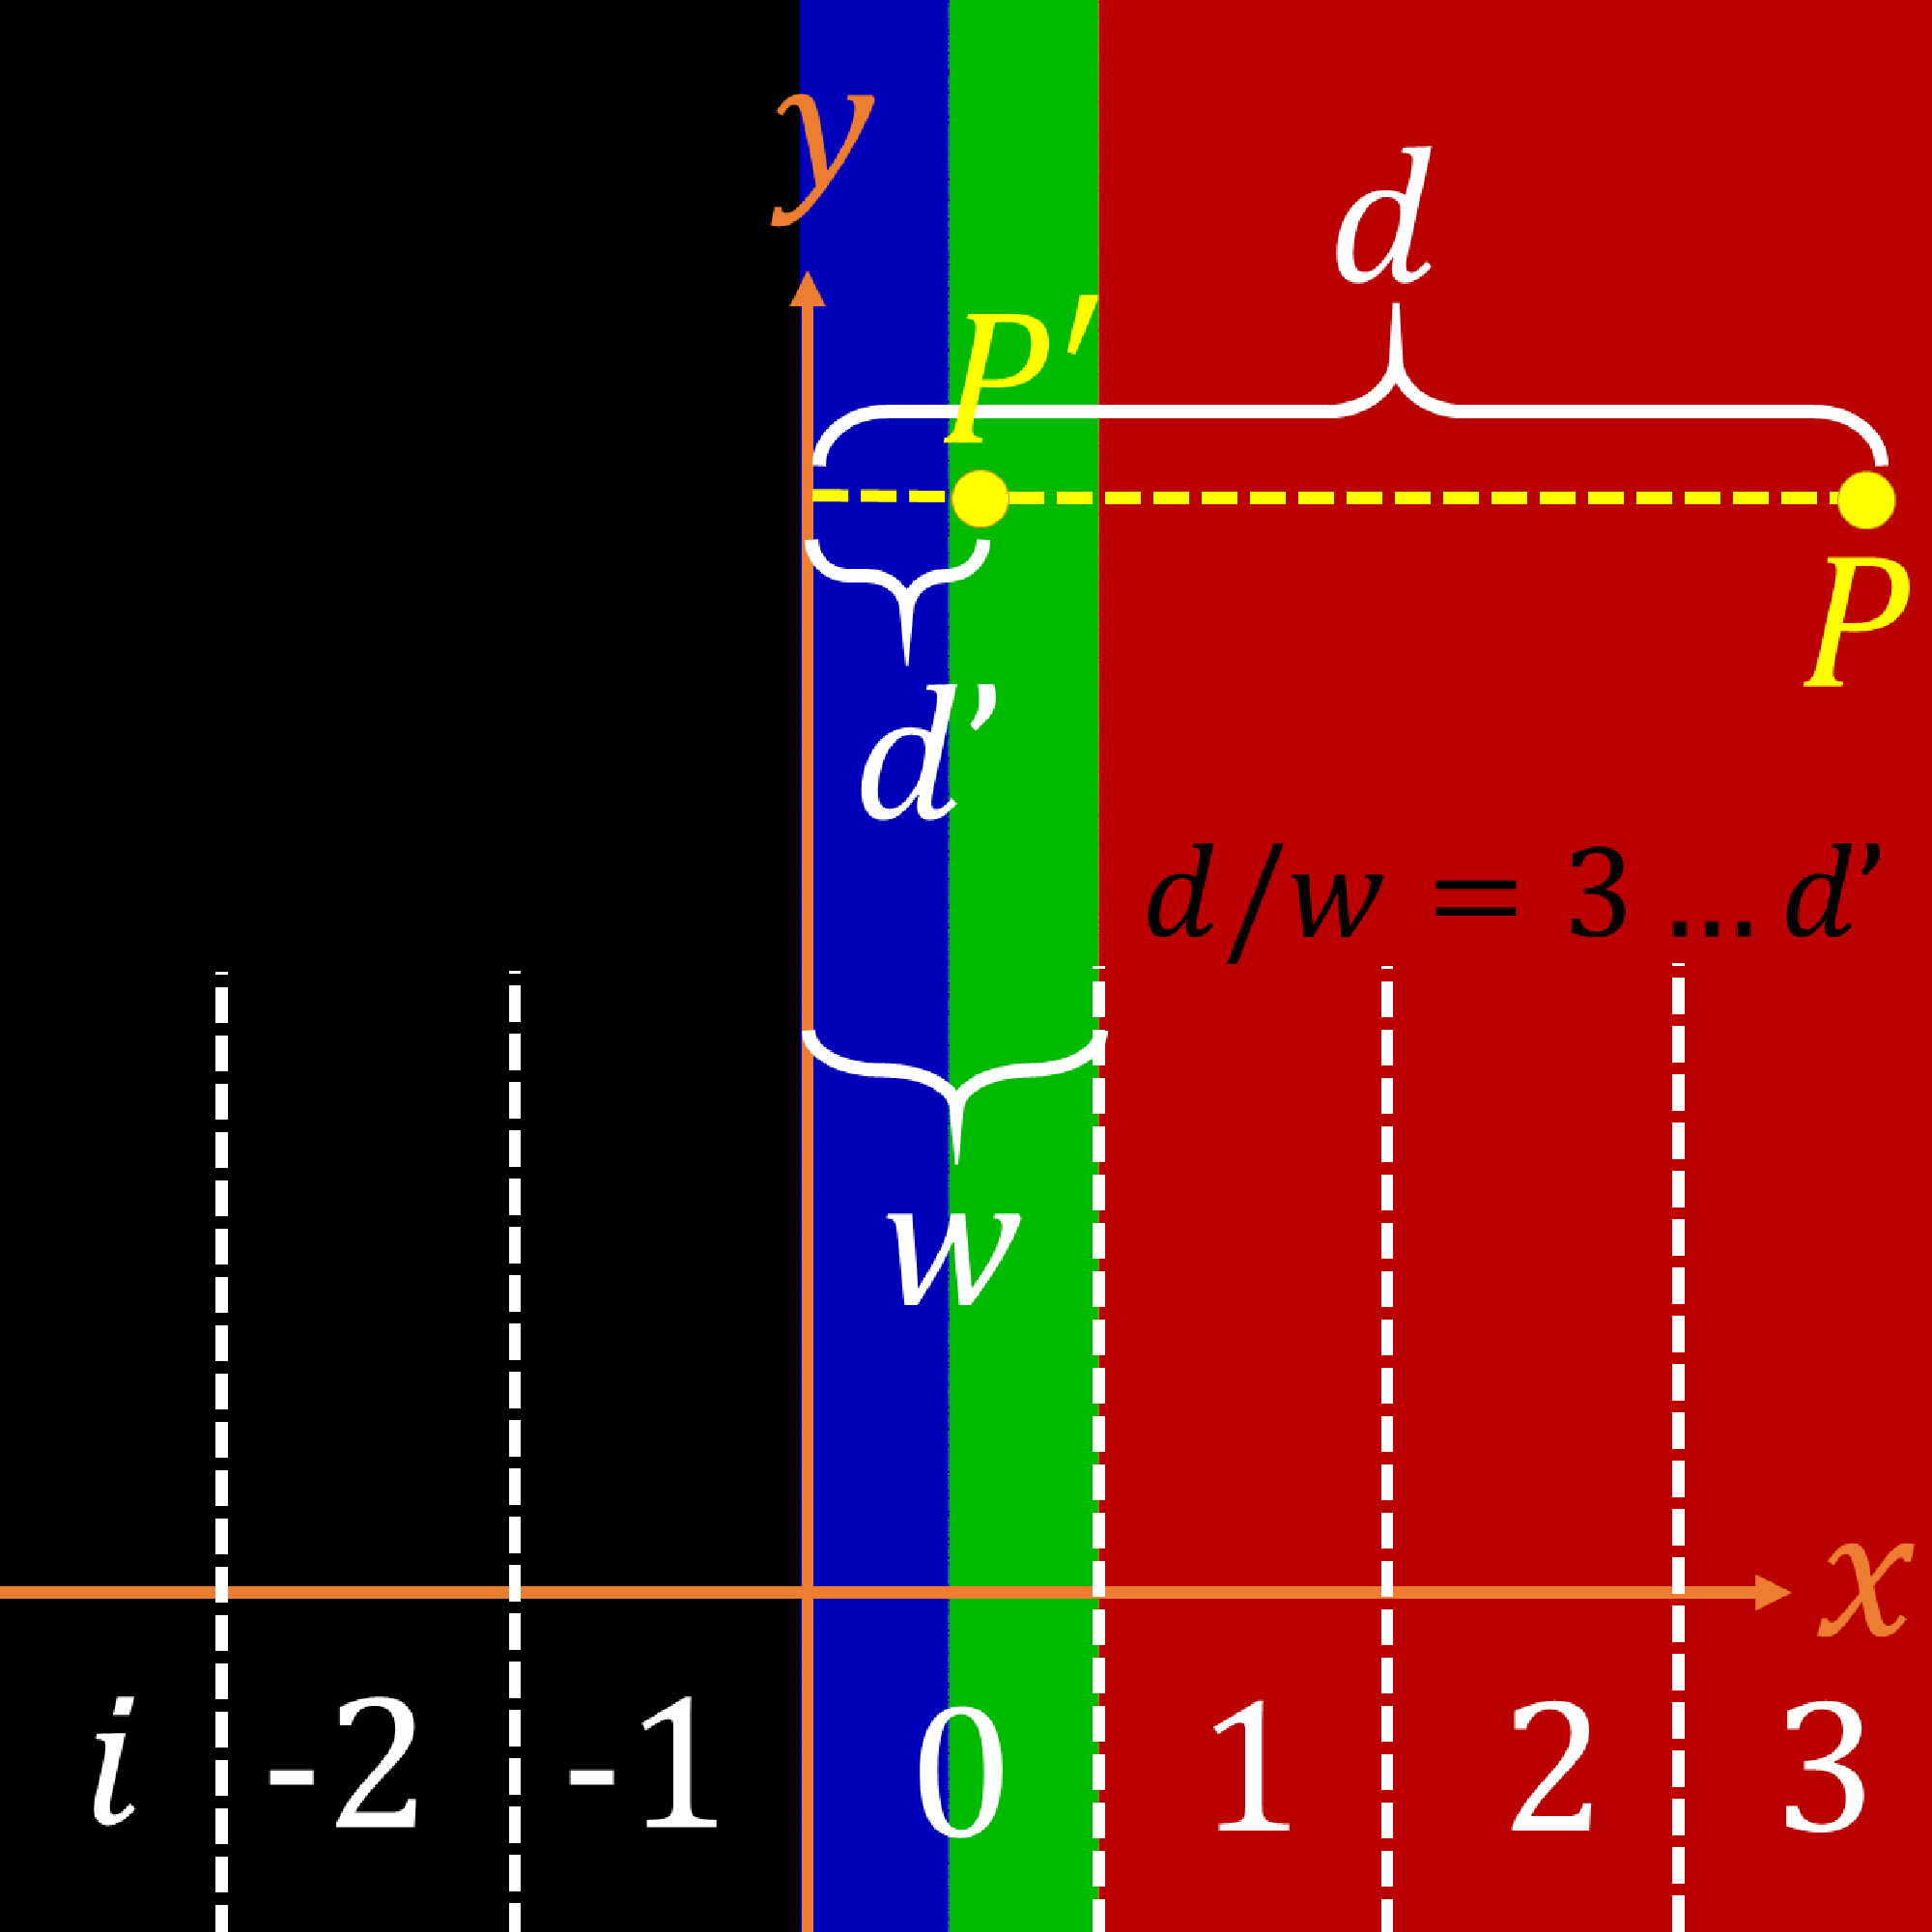
\includegraphics[width=1.5in, height=1.5in, keepaspectratio]{./img/application/optimization/parabolicMod.pdf}
  \end{center}
  \caption{\textit{Inverted parabolic generator.}}
  \label{fig:parabolicMod}
 \end{minipage}
 \hspace*{\fill}
 \begin{minipage}[t]{0.24\hsize}
   \begin{center}
    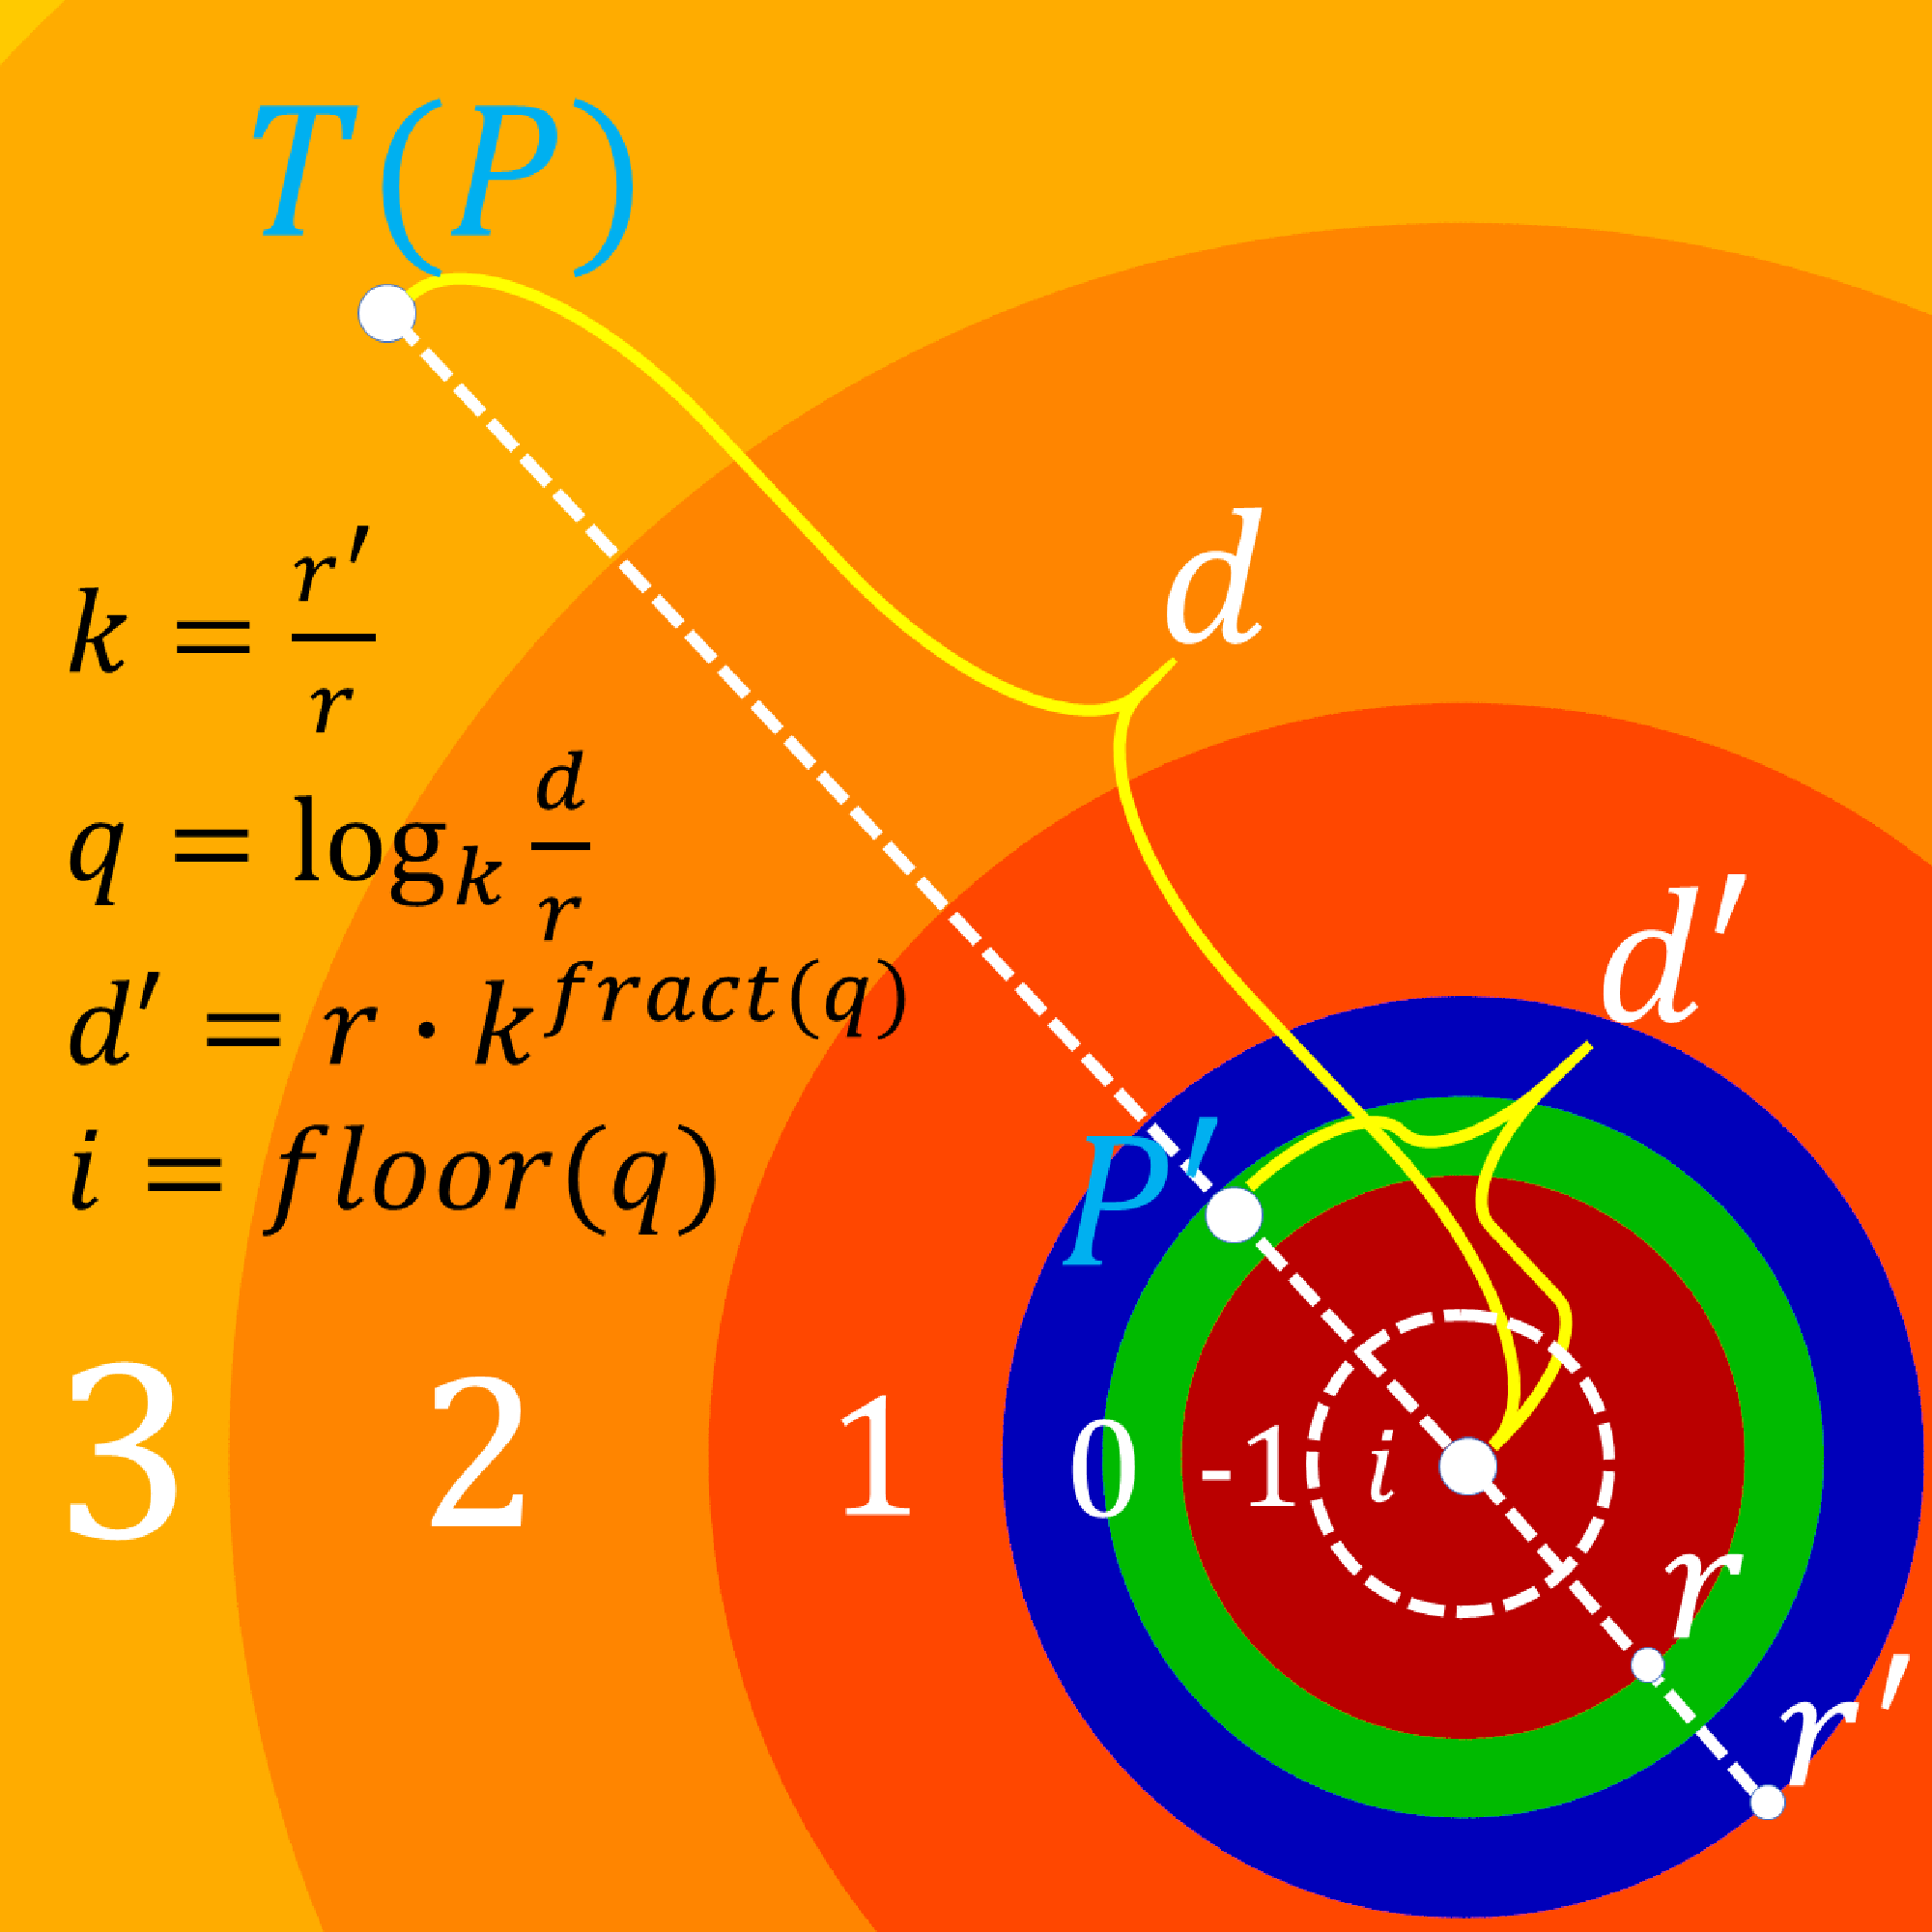
\includegraphics[width=1.5in, height=1.5in, keepaspectratio]{./img/application/optimization/hyperbolicMod.pdf}
   \end{center}
   \caption{\textit{Inverted hyperbolic generator.}}
   \label{fig:loxodromicMod}
 \end{minipage}
  \hspace*{\fill}
 \begin{minipage}[t]{0.24\hsize}
   \begin{center}
    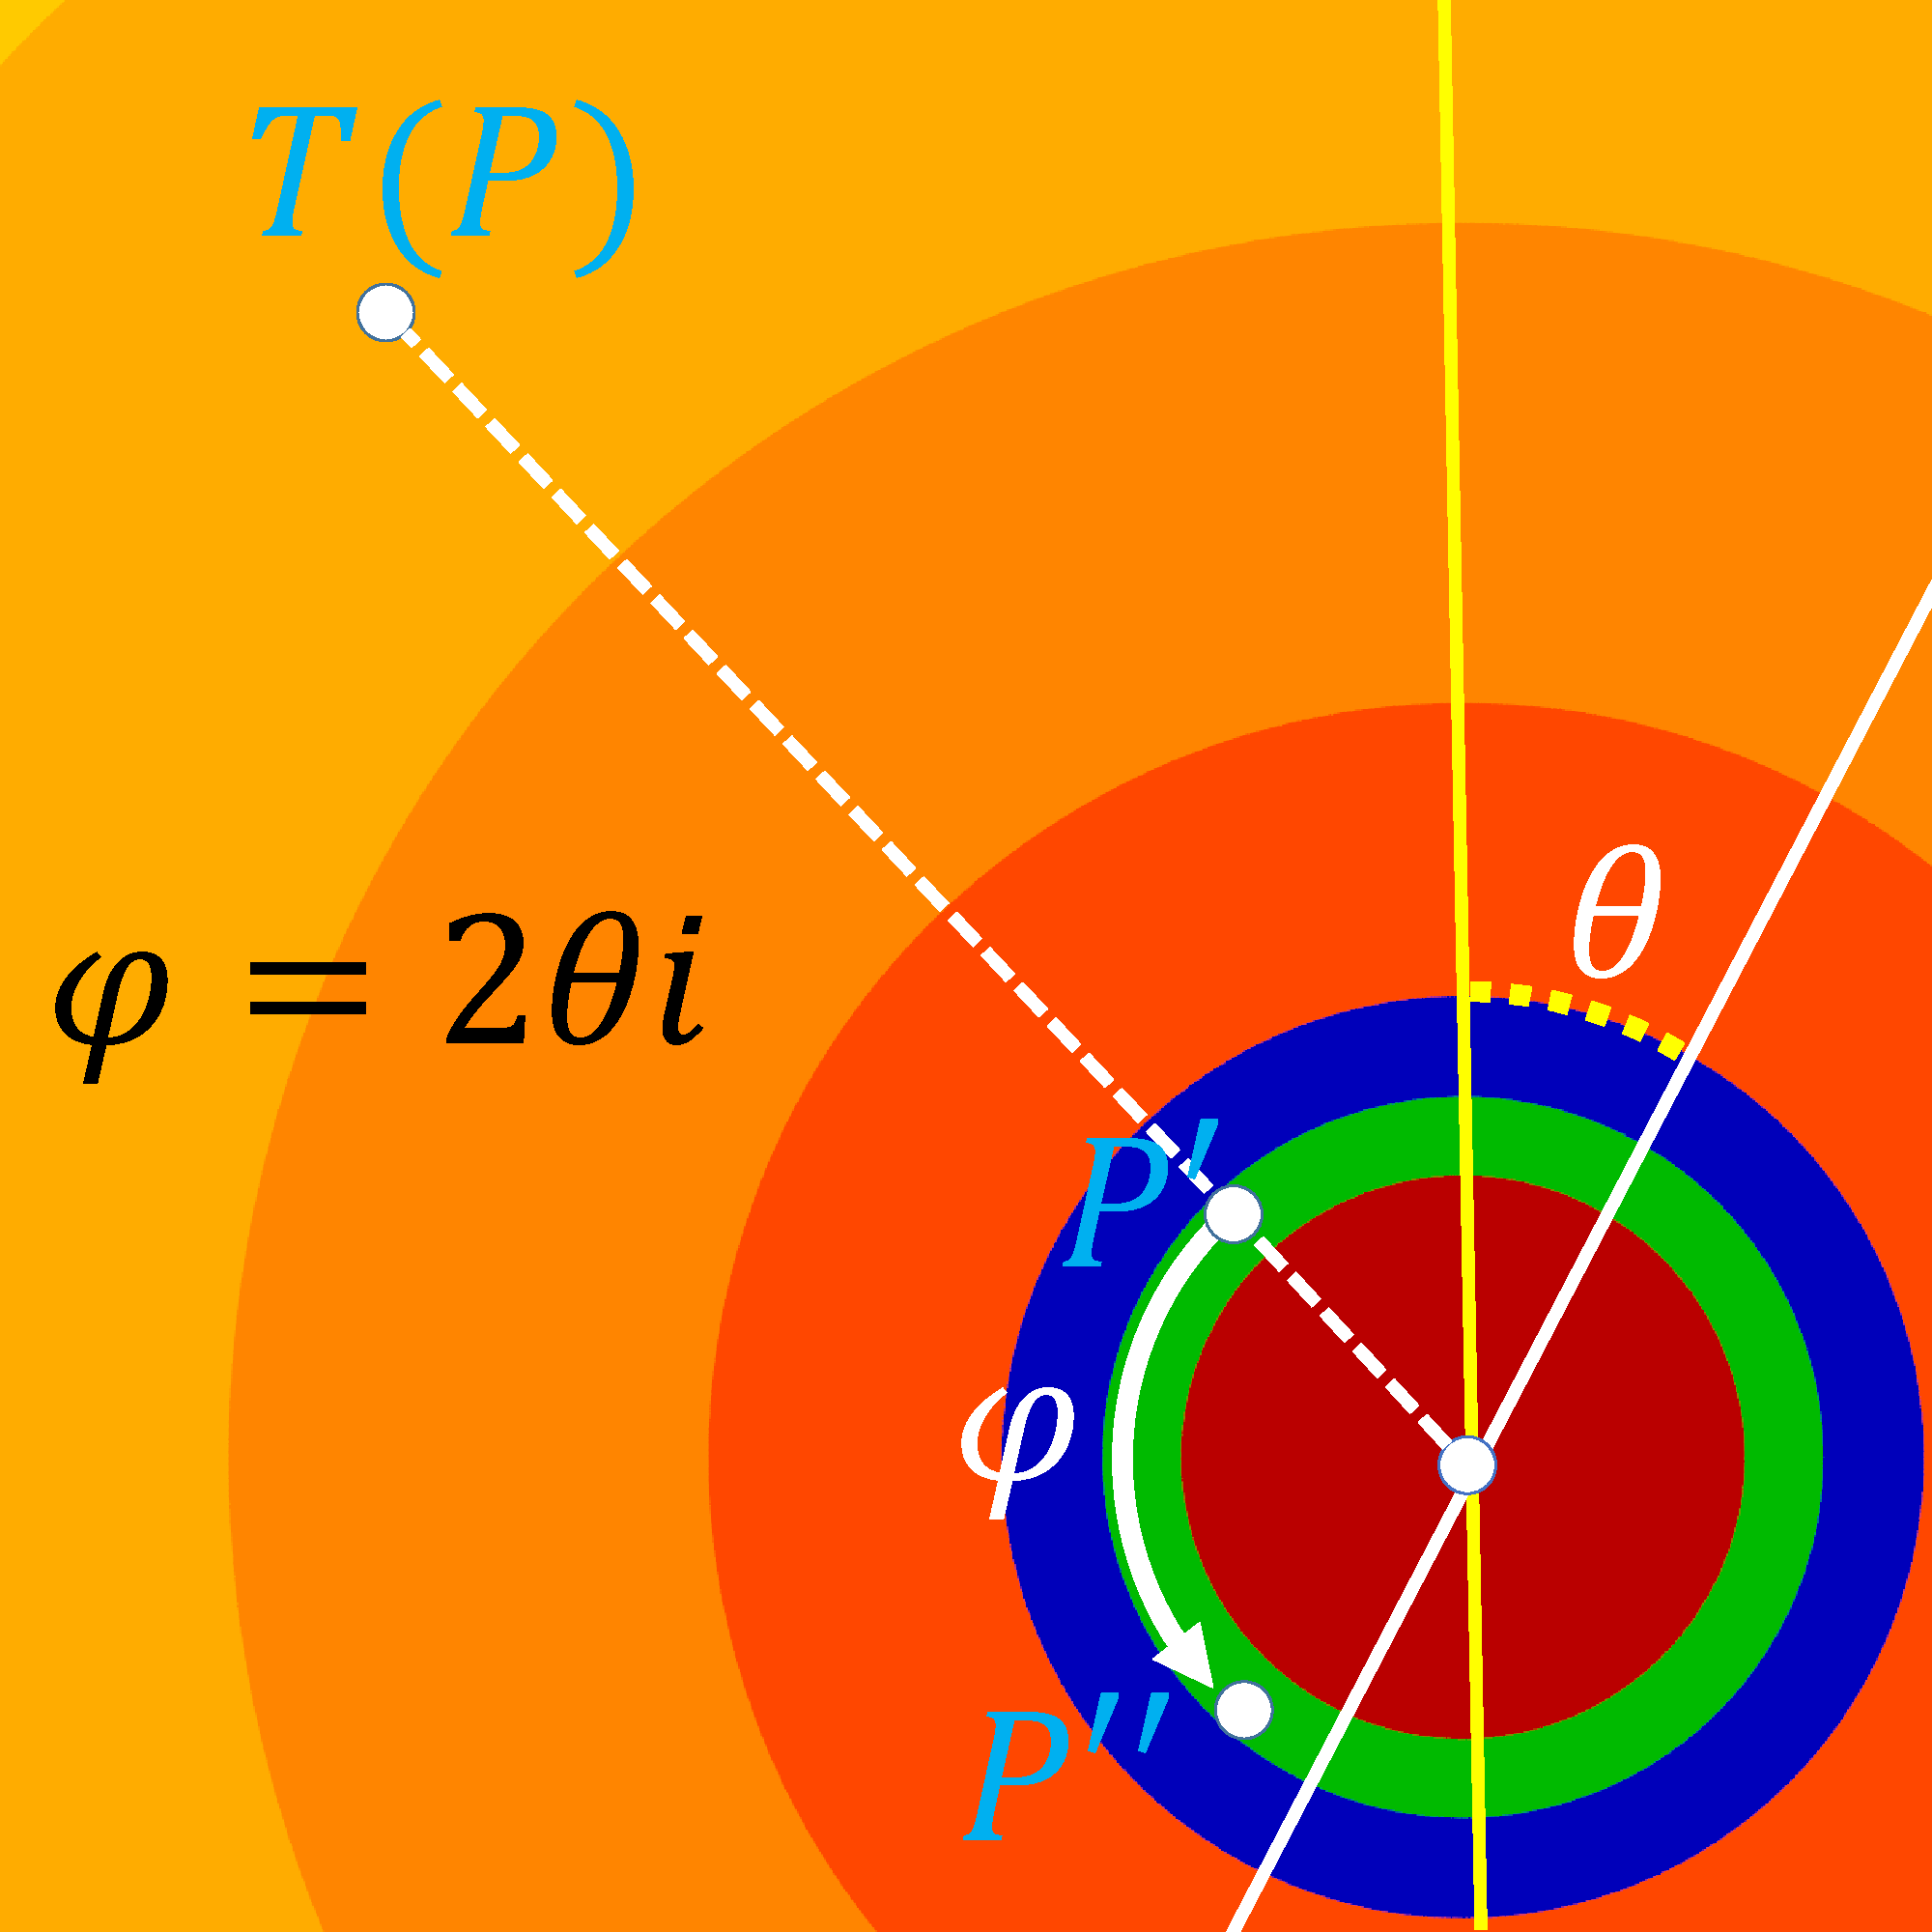
\includegraphics[width=1.5in, height=1.5in, keepaspectratio]{./img/application/optimization/loxodromicModRotation.pdf}
   \end{center}
   \caption{\textit{Inverted loxodromic generator.}}
   \label{fig:loxodromicRotationMod}
  \hspace*{\fill}
 \end{minipage}
\end{figure}


\subsubsection{Optimization}

 The maps of generators composed of some inversions
 can be optimized using proper conjugations.
 In this section, we introduce optimization techniques for two-dimensional
 generators.
 Optimized maps translate the points to the fundamental domain just one operation.
 Of course, we can also optimize three-dimensional generators in a similar manner to
 two-dimensional ones.
% Following examples are available on Shadertoy.
 % \footnote{IIS parallel translation example: \url{https://www.shadertoy.com/view/MtySzc}}
 % \footnote{IIS parabolic example: \url{https://www.shadertoy.com/view/llVSzd}}
 % \footnote{IIS loxodromic example: \url{https://www.shadertoy.com/view/4lGXDy}}

 \noindent\textbf{Parallel Translation\footnote{IIS Parallel Translation Example: \url{https://www.shadertoy.com/view/MtySzc}}.}
 Suppose that there are two parallel lines similar to Figure
 \ref{fig:translation2d}.
 We can map the point using a remainder instead of applying inversions
 repeatedly.
 First of all, we conjugate a given point by parallel translations and rotations to make the
 parallel lines perpendicular to the X-axis and aligned with the Y-axis.
 The conjugated lines are shown in Figure \ref{fig:translationMod}.
 Let $w$ be a distance between two lines, let $i$ be an index of a series
 of bands as in Figure \ref{fig:translationMod}, let $P$ be a given point, let
 $P'$ be a mapped point, and let $d$ and $d'$ be distances from the Y-axis.
 We divide $d$ by $w$ and get the remainder $d'$ and the
 quotient $i$.
 Finally, we calculate $P'$ using $d'$ and restore the $P'$ to the
 original geometry.

 \noindent\textbf{Parabolic\footnote{IIS Parabolic Transformation Example: \url{https://www.shadertoy.com/view/llVSzd}}.}
 Next, we consider parabolic transformations like Figure \ref{fig:parabolic2d}.
 Let $T$ be an inversion of a circle centered on the fixed point (the contact point of $C1$ and $C2$.)
 Applying $T$ to $C1$, $C2$, and $C1'$, we get parallel lines because
 the tangential point moves to the infinite point.
 We call the lines $TC1$, $TC2$, and $ TC1'$, and they are shown in
 Figure \ref{fig:parabolicMod}.
 The red line $TC1$ and the blue line $TC1'$ represent a parallel translation.
 The process of the map is as follows.
 Firstly, we apply $T$ to a given point $P$ and obtain $T(P)$.
 Then we translate $T(P)$ in the same way as parallel translations and get $P'$.
 Finally, we apply $T(= T^{-1}) $ to $P'$ again.

 \noindent\textbf{Loxodromic\footnote{IIS Loxodromic Transformation Example: \url{https://www.shadertoy.com/view/4lGXDy}}.}
 Finally, we consider hyperbolic
 transformations like Figure \ref{fig:hyperbolic2d}.
 Let $T$ be an inversion of a circle centered on one of the fixed
 points.
 We apply $T$ to $C1$, $C2$, and $C1'$.
 We call the images of them $TC1$, $TC2$, and $TC1'$.
 They are concentric circles centered on the inverted image
 of the other fixed point.
 They represent the real scaling.
 See Figure \ref{fig:loxodromicMod}.
 Let $P$ be a given point,
 let $P'$ be a mapped point,
 let $r$ and $r'$ be a radius of $TC1$ and $TC1'$,
 let $d$ and $d'$ be a distance from a center of $TC1$,
 let $k$ be a scaling factor,
 let $q$ be an exponential quotient, and let $i$ be an index of
 series of circles. They are calculated as follows:
 \begin{math}
  k = \frac{r'}{r},
  q = \log_{k} \frac{d}{r},
  d' = r \cdot k^{fracionalPart(q)},
  i = floor(q).
 \end{math}
 We calculate $P'$ using $d'$.
 When there is a loxodromic transformation similar to Figure \ref{fig:loxodromic2d},
 we also apply $T$ to $L$ and $C3$, and we call them $TL$ and $TC3$.
 See Figure \ref{fig:loxodromicRotationMod}.
 It represents a scaling by a complex number.
 The white line $TL$ and the yellow line $TC3$ are crossing
 through a center of the concentric circles.
 After we get $P'$, we calculate $P''$ by applying a rotation to $P'$.
 Let $\theta$ be the angle between $TL$ and $TC3$ and
 let $\varphi$ be the rotation angle.
 $\varphi$ is calculated as, $\varphi = 2 \theta i$.
 The process is shown below.
 Firstly, we apply $T$ to a given point and get $T(P)$.
 Next, we calculate $P'$ using $d'$.
 If there are crossing lines, we rotate $P'$ by $\varphi$ and get $P''$.
 Finally, we apply $T$ to $P'$ or $P''$ again.


\subsection{Sphairahedra and Three-dimensional Fractals}

\begin{figure}[h!tbp]
  \begin{minipage}[t]{0.25\textwidth}
   \centering
   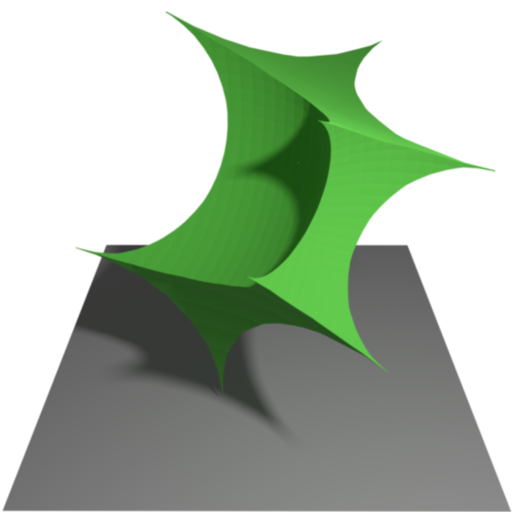
\includegraphics[height=1.2in, keepaspectratio]{./img/application/sphairahedron/cube.png}
   \caption{\textit{Cube-type sphairahedron.}}
   \label{fig:cubeSphaira}
  \end{minipage}
  \hspace*{\fill}
 \begin{minipage}[t]{0.75\textwidth}
  \begin{minipage}[t]{0.25\textwidth}
   \centering
   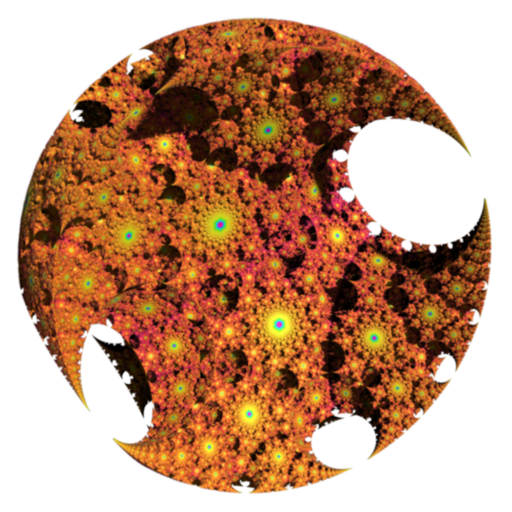
\includegraphics[height=1.2in,
   keepaspectratio]{./img/application/sphairahedron/quasi-sphere.png}
   \subcaption{}
  \end{minipage}
  \hspace*{\fill}
  \begin{minipage}[t]{0.25\textwidth}
   \centering
   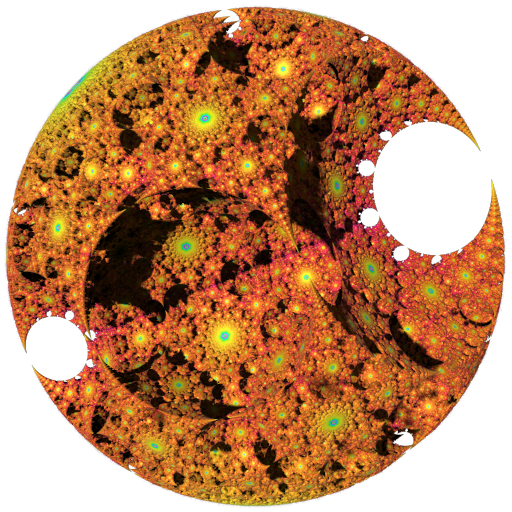
\includegraphics[height=1.2in,
   keepaspectratio]{./img/application/sphairahedron/other.png}
   \subcaption{}
  \end{minipage}
  \hspace*{\fill}
  \begin{minipage}[t]{0.25\textwidth}
   \centering
   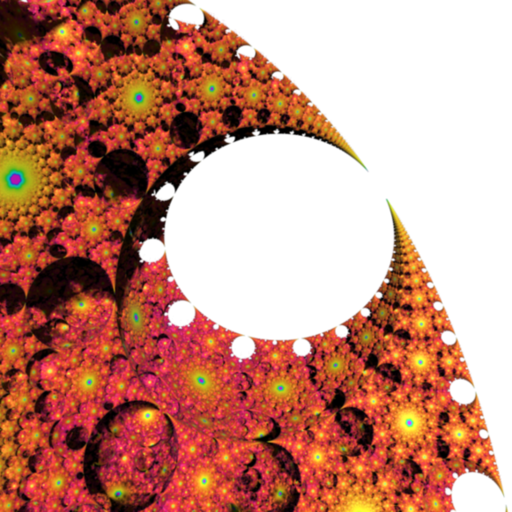
\includegraphics[height=1.2in,
   keepaspectratio]{./img/application/sphairahedron/quasi-sphereZoom.png}
   \subcaption{}
  \end{minipage}
  \hspace*{\fill}
  \caption{\textit{Images of a quasi-sphere rendered in different viewpoints.}}
  \label{fig:quasi-sphere}
 \end{minipage}
\end{figure}

\noindent In this section, we introduce an example of three-dimensional
tiling using IIS. 
We discussed this topic in \cite{bridges2018NakamuraAhara}. %\cite{bridgesbib2018:171}.
The paper is revised and included for this subsection.
The author gathers images, animation, and renderer for the fractals
at \url{https://sphairahedron.net}.

\subsubsection{Introduction}

In 2003, Kazushi Ahara and Yoshiaki Araki invented a new mathematical
concept called \textit{Sphairahedron} to introduce new kind of
three-dimensional fractals \cite{ahara2003sphairahedral}.

Sphairahedron is a coined word combining two words \textit{sphaira-}
(a prefix that means 'spherical') and \textit{-hedron} (a suffix comes
from 'polyhedron.')
In short, sphairahedron is a polyhedron with spherical faces.
See Figure \ref{fig:cubeSphaira}.
It shows cube-type sphairahedron. 
As we can see, each face of the cube is a part of a sphere.

We can make a tiling pattern of sphairahedra using inversion about their
spherical faces.
In many cases, the boundary of the tiling converges to a three-dimensional fractal
shape as shown in Figure \ref{fig:quasi-sphere}.
The union of all the tiles is mostly homeomorphic to a three-dimensional
ball. Thus, this is called a \textit{quasi-sphere}.
Also, the boundary of the fractal is the limit set of the sphere
inversion group.

Mathematically speaking, we consider a Coxeter-like group generated by the
inversions in all of the spherical faces of the sphairahedron, and
we obtain the tiling after transforming the original sphairahedron by
each element of the group.
Also, under some technical conditions, the group is called a
\textit{quasi-fuchsian group} and the limit set a \textit{quasi-fuchsian
fractal}.

A quasi-fuchsian fractal is one of the three-dimensional
fractals at an early era of visualizing fractals by computer.
The video\footnote{Quasi-fuchsian fractals:
\url{https://www.youtube.com/watch?v=3lcO9zRCv-4}}
posted by Ahara and Araki shows the fractal based on a cube-type
sphairahedron in the case of only quasi-fuchsian.
However, there are sphairahedra based on other types of polyhedra, and
we can allow tiles to self-intersect each other, that is, the group is
not quasi-fuchsian.
In this way, we can see more varieties of fractal patterns
than proposed by Ahara and Araki.
         
The three-dimensional tiling of hyperbolic polyhedra is well known. 
In comparison to this, sphairahedra 
and their tiling patterns are originated from four-dimensional
hyperbolic geometry.
The rise in dimension brings complexity and difficulty for
visualization, but visualized shapes have impressive structures.
In this paper, we will introduce a variety of sphairahedra and fractal shapes
generated by them. 
                                                                                   
\subsubsection{Sphairahedron}

\begin{figure}[h!tbp]
 \begin{minipage}[t]{0.6\textwidth}
  \centering
  \begin{minipage}[t]{0.19\textwidth}
   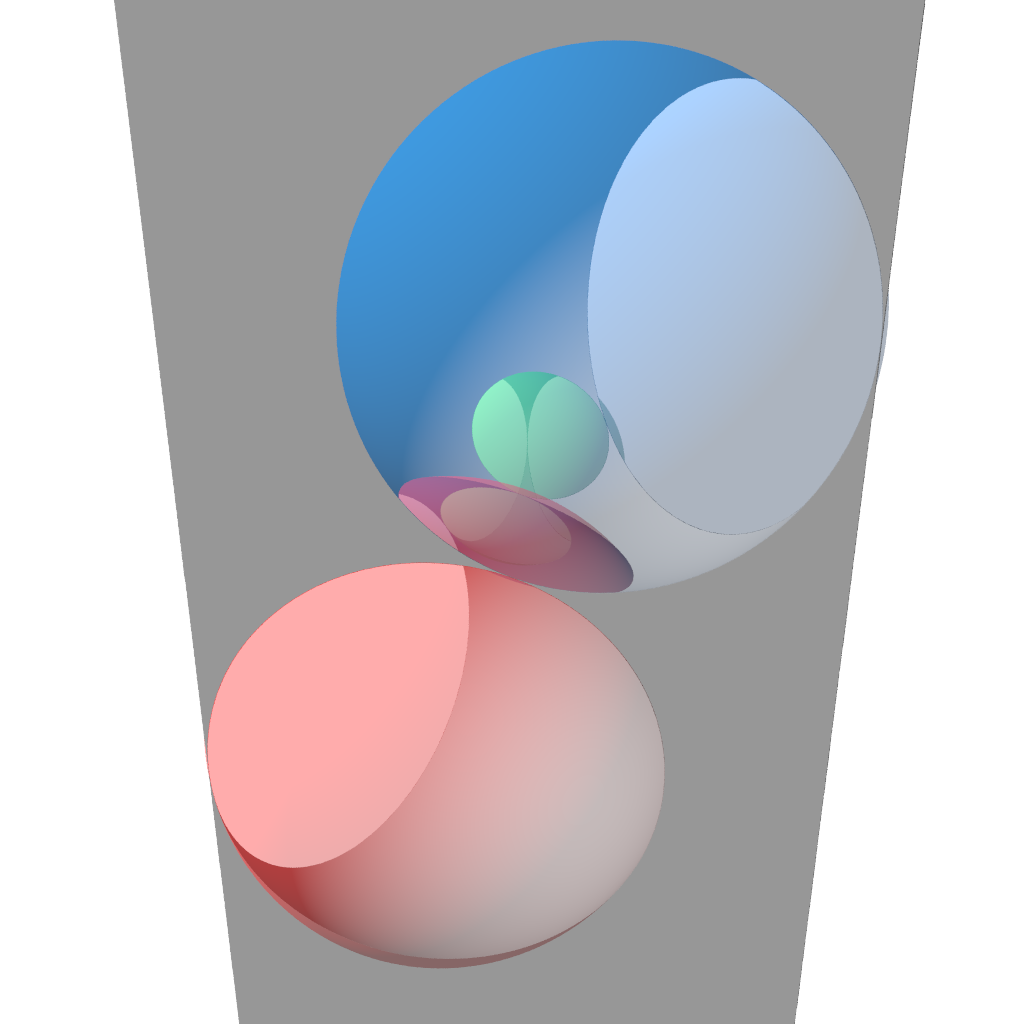
\includegraphics[width=1.2in, height=1.2in, keepaspectratio]
   {./img/application/sphairahedron/sphairahedron/sphairaAll.png}
   \subcaption{\textit{$A$}}
   \label{fig:sphairaPrismAll}
  \end{minipage}
  \hspace*{\fill}
   \begin{minipage}[t]{0.19\textwidth}
   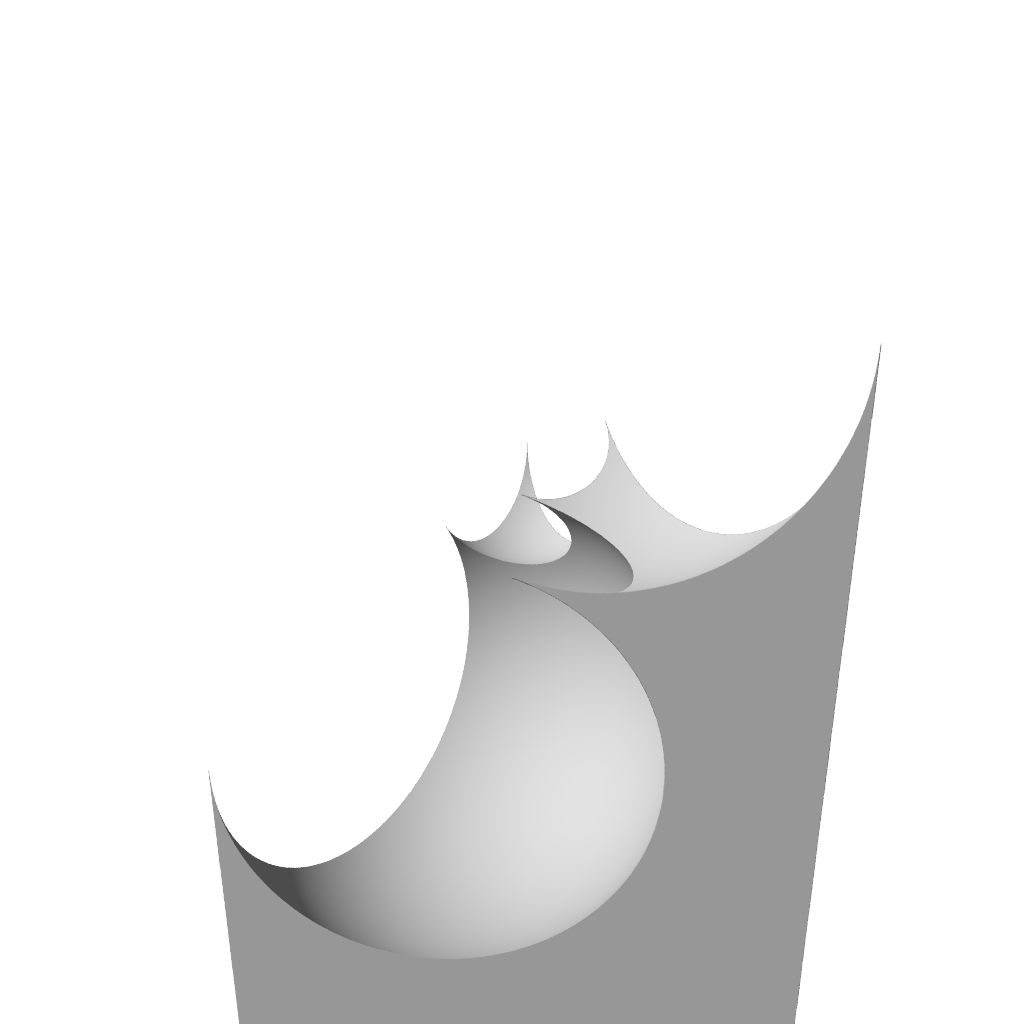
\includegraphics[width=1.2in, height=1.2in, keepaspectratio]
   {./img/application/sphairahedron/sphairahedron/sphairaHalf.png}
   \subcaption{\textit{Infinite type}}
   \label{fig:sphairaPrismHalf}
  \end{minipage}
  \hspace*{\fill}
  \begin{minipage}[t]{0.19\textwidth}
   
\includegraphics[width=1.2in, height=1.2in, keepaspectratio]
   {./img/application/sphairahedron/sphairahedron/sphairahedron.png}
   \subcaption{\textit{Finite type}}
   \label{fig:sphairahedronFinite}
  \end{minipage}
  \hspace*{\fill}
  \caption{\textit{Sphairahedron.}}
  \label{fig:sphairahedron}
 \end{minipage}
 \begin{minipage}[t]{0.4\textwidth}
  \centering
  \begin{minipage}[t]{0.19\textwidth}
   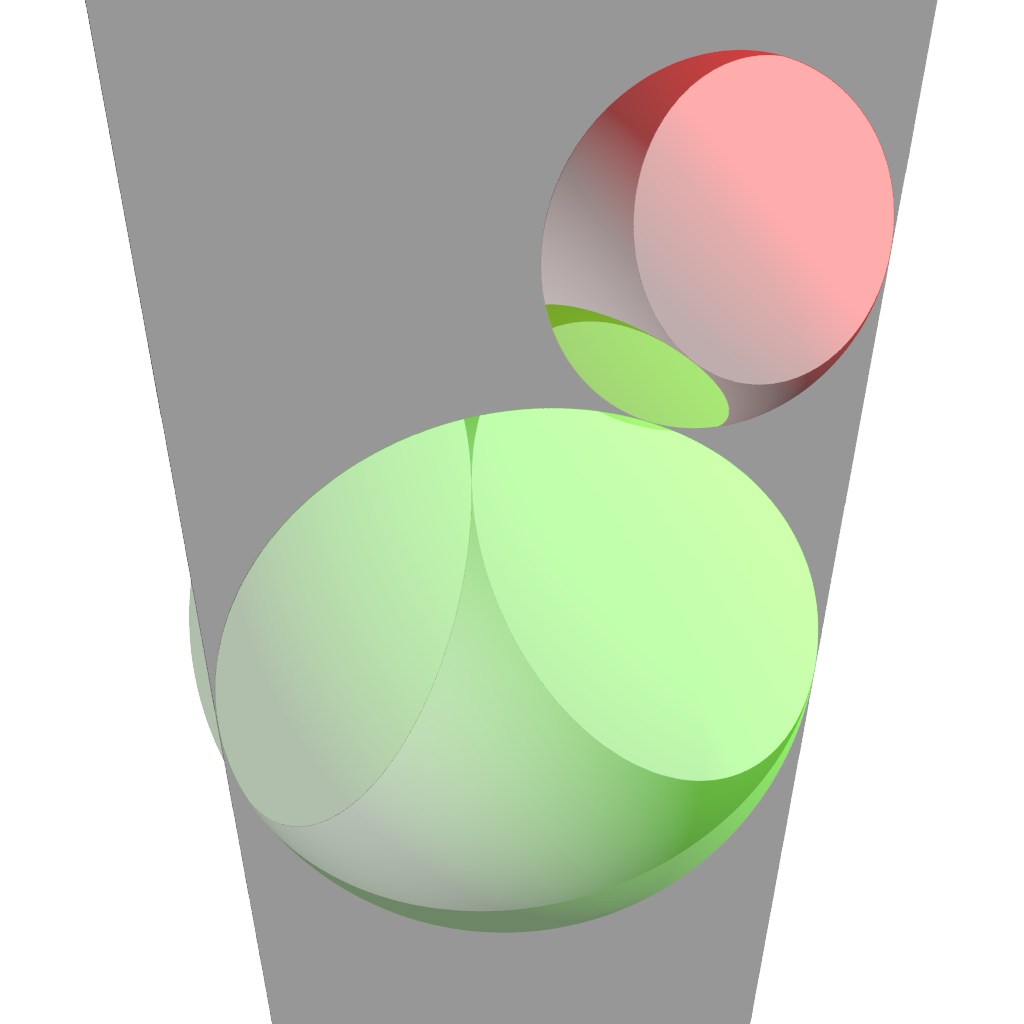
\includegraphics[width=1.2in, height=1.2in, keepaspectratio]{./img/application/sphairahedron/sphairahedron/semiSphairaAll.png}
   \subcaption{\textit{$A$}}
   \label{fig:semi-sphairaAll}
  \end{minipage}
  \hspace*{\fill}
  \begin{minipage}[t]{0.19\textwidth}
   
\includegraphics[width=1.2in, height=1.2in, keepaspectratio]{./img/application/sphairahedron/sphairahedron/semiSphairaHalf.png}
   \subcaption{\textit{Infinite type}}
   \label{fig:semi-sphairaHalf}
  \end{minipage}
  \hspace*{\fill}
  \caption{\textit{Semi-sphairahedron.}}
  \label{fig:semi-sphairahedron}
 \end{minipage}
\end{figure}

\noindent
First of all, we will describe the definition of a sphairahedron.
Let $S^3 = R^3 \cup \{\infty\}$ be a three-dimensional sphere and let
$\overline{D_1},~\overline{D_2},~...,~\overline{D_p}$ be some three-dimensional closed balls.
We consider the complement $A$ of the union of these balls, that is,
$A = S^3 - (\overline{D_1} \cup \overline{D_2} \cup ... \cup \overline{D_p})$.
If $A$ is composed of simply-connected two components;
in other words, $A$ has two connected components and the first homology
group of each component is trivial, we call one side of $A$
a sphairahedron.

The image in Figure \ref{fig:sphairahedron}\subref{fig:sphairaPrismAll}
is an example of $A$.
We hollow out the $S^3$ with six balls: we remove three half space
(three balls with infinite radius,) from $S^3$ and obtain the prism of
infinite length, and we scoop out the prism by the remaining
three-colored transparent balls as in Figure \ref{fig:sphairahedron}\subref{fig:sphairaPrismAll}.
$A$ is composed of two parts, and each of the components is simply connected.
Since it has six faces, and these faces are arranged as those of faces of
a cube, it is called a cube-type sphairahedron.
Especially, the sphairahedron shown in Figure \ref{fig:sphairahedron}\subref{fig:sphairaPrismHalf}
is also called an \textit{infinite type sphairahedron},
because one of the vertices of the sphairahedron is at the infinity.
Similarly, the shape hollowed out by six finite balls in Figure
\ref{fig:sphairahedron}\subref{fig:sphairahedronFinite} is called a
\textit{finite type sphairahedron}.

Moreover, we can loosen the definition of sphairahedron,
that is, the case $A$ has simply connected three or more components.
Figure \ref{fig:semi-sphairahedron}\subref{fig:semi-sphairaAll} shows an
example of $A$ with simply connected three components.
It is the $S^3$ scooped out by five balls and a pentahedral prism type
sphairahedron.
We divide $A$ so that one part of $A$ has five faces as shown in
Figure \ref{fig:semi-sphairahedron}\subref{fig:semi-sphairaHalf}.
We can regard the resulting shape as a singular case of a pentahedron,
and we call it a \textit{semi-sphairahedron}.

\begin{figure}[H]
 \begin{minipage}[t]{0.19\textwidth}
  \centering
  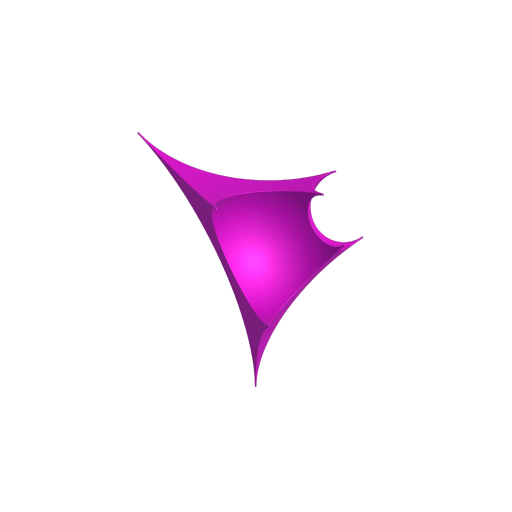
\includegraphics[width=1.1in, height=1.1in, keepaspectratio]{./img/application/sphairahedron/finiteProcess/step1.png}
  \subcaption{\textit{Step 1}}
  \label{fig:sphaira-step1}
 \end{minipage}
 \hspace*{\fill}
 \begin{minipage}[t]{0.19\textwidth}
  \centering
  \includegraphics[width=1.1in, height=1.1in, keepaspectratio]{./img/application/sphairahedron/finiteProcess/step2.png}
  \subcaption{\textit{Step 2}}
  \label{fig:sphaira-step2}
 \end{minipage}
 \hspace*{\fill}
 \begin{minipage}[t]{0.19\textwidth}
  \centering
  \includegraphics[width=1.1in, height=1.1in, keepaspectratio]{./img/application/sphairahedron/finiteProcess/step5.png}
  \subcaption{\textit{Step 5}}
  \label{fig:sphaira-step5}
 \end{minipage}
 \hspace*{\fill}
 \begin{minipage}[t]{0.19\textwidth}
  \centering
  \includegraphics[width=1.1in, height=1.1in, keepaspectratio]{./img/application/sphairahedron/finiteProcess/step10.png}
  \subcaption{\textit{Step 10}}
  \label{fig:sphaira-step10}
 \end{minipage}
 \hspace*{\fill}
 \begin{minipage}[t]{0.19\textwidth}
  \centering
  \includegraphics[width=1.1in, height=1.1in, keepaspectratio]{./img/application/sphairahedron/finiteProcess/final.png}
  \subcaption{\textit{Final image}}
  \label{fig:sphaira-final}
 \end{minipage}
 \hspace*{\fill}
 \caption{\textit{Tiling of a finite cube-type sphairahedron.}}
 \label{fig:sphairahedronTile}
\end{figure}

\begin{figure}[h!tbp]
 \begin{minipage}[t]{0.19\textwidth}
  \centering
  \includegraphics[height=1.2in, keepaspectratio]{./img/application/sphairahedron/constructFractal/terrainProcess/step1.png}
  \subcaption{\textit{Step 1}}
  \label{fig:terrainStep1}
 \end{minipage}
 \hspace*{\fill}
 \begin{minipage}[t]{0.19\textwidth}
  \centering
  \includegraphics[height=1.2in, keepaspectratio]{./img/application/sphairahedron/constructFractal/terrainProcess/step2.png}
  \subcaption{\textit{Step 2}}
  \label{}
 \end{minipage}
 \hspace*{\fill}
 \begin{minipage}[t]{0.19\textwidth}
  \centering
  \includegraphics[height=1.2in, keepaspectratio]{./img/application/sphairahedron/constructFractal/terrainProcess/step5.png}
  \subcaption{\textit{Step 5}}
  \label{}
 \end{minipage}
 \hspace*{\fill}
 \begin{minipage}[t]{0.19\textwidth}
  \centering
  \includegraphics[height=1.2in, keepaspectratio]{./img/application/sphairahedron/constructFractal/terrainProcess/step10.jpg}
  \subcaption{\textit{Step 10}}
  \label{fig:terrainStep10}
 \end{minipage}
 \hspace*{\fill}
 \begin{minipage}[t]{0.19\textwidth}
  \centering
  \includegraphics[height=1.2in, keepaspectratio]{./img/application/sphairahedron/constructFractal/terrainProcess/final.jpg}
  \subcaption{\textit{Final image}}
  \label{figsphairaPrismFinal}
 \end{minipage}
 \caption{\textit{Tiling of a cube-type infinite sphairahedron.}}
 \label{fig:sphairahedralPrismTile}
\end{figure}


\subsubsection{Construct Fractal}

In Figure \ref{fig:sphairahedronTile} we show a process of the tiling of
sphairahedra.
The sphairahedron presented in Figure
\ref{fig:sphairahedronTile}\subref{fig:sphaira-step1} has six spherical
faces.
We apply inversions in each spherical face to original sphairahedron,
and we obtain new six sphairahedra surrounding the initial sphairahedron
as shown in Figure
\ref{fig:sphairahedronTile}\subref{fig:sphaira-step2}.
Next, we apply inversions in each of the new faces to the new sphairahedra,
and we obtain more sphairahedra.
We continue iterating inversions, and finally, we get a three-dimensional
fractal shape as presented in Figure
\ref{fig:sphairahedronTile}\subref{fig:sphaira-final}.

\begin{figure}[h!tbp]
 \begin{minipage}[t]{0.5\textwidth}
 \centering
 \includegraphics[height=1.3in, keepaspectratio]{./img/application/sphairahedron/constructFractal/terrain.jpg}
 \caption{\textit{Fractal terrain besed on the infinite sphairahedron in Figure \ref{fig:sphairahedralPrismTile}.}}
 \label{fig:terrain}
 \end{minipage}
 \hspace*{\fill}
 \begin{minipage}[t]{0.5\textwidth}
 \centering
 \includegraphics[height=1.3in, keepaspectratio]{./img/application/sphairahedron/constructFractal/semi-terrain2.png}
 \caption{\textit{Fractal terrain based on the infinite semi-sphairahedron in
  Figure \ref{fig:semi-sphairahedron}.}}
 \label{fig:semi-terrain}
 \end{minipage}
 \hspace*{\fill}
\end{figure}

\begin{figure}[htbp]
 \begin{minipage}[t]{0.24\textwidth}
  \centering
  \includegraphics[width=1.5in, height=1.5in, keepaspectratio]{./img/application/sphairahedron/derivation/graphTri.png}
 \caption{\textit{Polyhedral Graph for infinite sphairahedron.}}
 \label{fig:graph}
 \end{minipage}
 \hspace*{\fill}
 \begin{minipage}[t]{0.24\textwidth}
  \centering
\begin{tikzpicture}[line cap=round,line join=round,>=triangle
 45,x=1cm,y=1cm]
\draw[->,color=black] (-1.7879982790065765,0) --
 (1.9702145209475532,0);\foreach \x in
 {-1.5,-1,-0.5,0.5,1, 1.5}\draw[shift={(\x,0)},color=black] (0pt,2pt) --
 (0pt,-2pt);\draw[->,color=black] (0,-1.545344552024163) --
 (0,1.596018730612241);\foreach \y in
 {-1.5,-1,-0.5,0.5,1}\draw[shift={(0,\y)},color=black] (2pt,0pt) --
 (-2pt,0pt);\clip(-1.7879982790065765,-1.545344552024163) rectangle
 (1.9702145209475532,1.596018730612241);
 \draw[line width=0pt,dash
 pattern=on 1pt off 1pt,color=wqwqwq,fill=wqwqwq,fill
 opacity=0.2](0.6124404939620633,1.2250488973986702)--(0.5780045693371592,1.201976720533932)--(0.48395223524051034,1.1411715588334386)--(0.3922496978948061,1.0840803412862037)--(0.3024810567829962,1.0303728832892913)--(0.21426108965273136,0.9797570133882552)--(0.12722913340978584,0.9319732558979307)--(0.041043725782849066,0.8867903818025842)--(-0.044622170473813075,0.8440016669054409)--(-0.13008550904331037,0.803421729447473)--(-0.21565719357168806,0.7648838451357799)--(-0.3016459143925736,0.728237657560985)--(-0.3883618897293505,0.6933472177017516)--(-0.47612060746630336,0.6600892986235605)--(-0.5652466626682917,0.6283519413348821)--(-0.6125593295934284,0.6125593295934274)--(-0.6125593295934281,0.6125593295934274)--(-0.6283519413348823,0.5652466626682917)--(-0.6600892986235609,0.4761206074663035)--(-0.6933472177017517,0.38836188972935043)--(-0.7282376575609851,0.30164591439257366)--(-0.76488384513578,0.21565719357168817)--(-0.8034217294474734,0.13008550904331026)--(-0.844001666905441,0.0446221704738127)--(-0.8867903818025843,-0.041043725782849046)--(-0.9319732558979311,-0.12722913340978573)--(-0.9797570133882553,-0.2142610896527315)--(-1.0303728832892916,-0.3024810567829966)--(-1.084080341286204,-0.3922496978948064)--(-1.1411715588334388,-0.4839522352405108)--(-1.2019767205339325,-0.5780045693371595)--(-1.2250488973986702,-0.6124404939620631)--(-1.2250488973986706,-0.6124404939620631)--(-1.2108922257978854,-0.6193779958458375)--(-1.1604559044732938,-0.646297715500365)--(-1.1124111198346147,-0.6742111676405248)--(-1.066591712200237,-0.7031744119339248)--(-1.022846566109127,-0.7332478055364395)--(-0.9810379453638532,-0.7644964229409448)--(-0.9410400444000885,-0.7969905260281707)--(-0.9027377238859907,-0.8308060914652986)--(-0.8660254037844385,-0.8660254037844385)--(-0.8308060914652985,-0.9027377238859905)--(-0.7969905260281707,-0.9410400444000885)--(-0.7644964229409446,-0.9810379453638532)--(-0.7332478055364394,-1.0228465661091268)--(-0.7031744119339249,-1.0665917122002369)--(-0.6742111676405248,-1.1124111198346147)--(-0.6462977155003651,-1.1604559044732943)--(-0.6193779958458375,-1.2108922257978856)--(-0.6124404939620633,-1.2250488973986702)--(-0.6124404939620631,-1.2250488973986702)--(-0.5780045693371592,-1.201976720533932)--(-0.4839522352405105,-1.1411715588334386)--(-0.3922496978948061,-1.0840803412862035)--(-0.3024810567829962,-1.0303728832892913)--(-0.21426108965273136,-0.9797570133882552)--(-0.12722913340978584,-0.9319732558979309)--(-0.041043725782849066,-0.886790381802584)--(0.044622170473813075,-0.8440016669054407)--(0.13008550904331037,-0.803421729447473)--(0.21565719357168806,-0.7648838451357799)--(0.3016459143925736,-0.7282376575609851)--(0.3883618897293505,-0.6933472177017513)--(0.47612060746630336,-0.6600892986235605)--(0.5652466626682917,-0.6283519413348821)--(0.6125593295934256,-0.6125593295934283)--(0.6125593295934276,-0.6125593295934283)--(0.6283519413348823,-0.5652466626682915)--(0.6600892986235609,-0.4761206074663035)--(0.6933472177017517,-0.38836188972935043)--(0.7282376575609851,-0.30164591439257366)--(0.7648838451357798,-0.21565719357168817)--(0.8034217294474734,-0.13008550904331026)--(0.844001666905441,-0.0446221704738127)--(0.8867903818025843,0.041043725782849046)--(0.9319732558979312,0.12722913340978573)--(0.9797570133882553,0.21426108965273166)--(1.0303728832892918,0.3024810567829966)--(1.084080341286204,0.3922496978948064)--(1.1411715588334388,0.4839522352405108)--(1.201976720533932,0.5780045693371596)--(1.22504889739867,0.6124404939620635)--(1.2108922257978854,0.6193779958458375)--(1.160455904473294,0.6462977155003651)--(1.1124111198346147,0.6742111676405247)--(1.066591712200237,0.7031744119339249)--(1.022846566109127,0.7332478055364395)--(0.9810379453638535,0.7644964229409446)--(0.9410400444000883,0.7969905260281708)--(0.9027377238859907,0.8308060914652984)--(0.8660254037844384,0.8660254037844385)--(0.8308060914652985,0.9027377238859907)--(0.7969905260281706,0.9410400444000886)--(0.7644964229409443,0.9810379453638535)--(0.7332478055364395,1.0228465661091268)--(0.7031744119339249,1.066591712200237)--(0.674211167640525,1.1124111198346147)--(0.6462977155003649,1.160455904473294)--(0.6193779958458375,1.2108922257978856)--(0.6124404939620633,1.2250488973986702);\draw[line
 width=0pt,dash pattern=on 1pt off 1pt,color=wqwqwq,fill=wqwqwq,fill
 opacity=0.2](0.6124404939620633,1.2250488973986702)--(0.5780045693371592,1.201976720533932)--(0.48395223524051034,1.1411715588334386)--(0.3922496978948061,1.0840803412862037)--(0.3024810567829962,1.0303728832892913)--(0.21426108965273136,0.9797570133882552)--(0.12722913340978584,0.9319732558979307)--(0.041043725782849066,0.8867903818025842)--(-0.044622170473813075,0.8440016669054409)--(-0.13008550904331037,0.803421729447473)--(-0.21565719357168806,0.7648838451357799)--(-0.3016459143925736,0.728237657560985)--(-0.3883618897293505,0.6933472177017516)--(-0.47612060746630336,0.6600892986235605)--(-0.5652466626682917,0.6283519413348821)--(-0.6125593295934284,0.6125593295934274)--(-0.6125593295934281,0.6125593295934274)--(-0.6283519413348823,0.5652466626682917)--(-0.6600892986235609,0.4761206074663035)--(-0.6933472177017517,0.38836188972935043)--(-0.7282376575609851,0.30164591439257366)--(-0.76488384513578,0.21565719357168817)--(-0.8034217294474734,0.13008550904331026)--(-0.844001666905441,0.0446221704738127)--(-0.8867903818025843,-0.041043725782849046)--(-0.9319732558979311,-0.12722913340978573)--(-0.9797570133882553,-0.2142610896527315)--(-1.0303728832892916,-0.3024810567829966)--(-1.084080341286204,-0.3922496978948064)--(-1.1411715588334388,-0.4839522352405108)--(-1.2019767205339325,-0.5780045693371595)--(-1.2250488973986702,-0.6124404939620631)--(-1.2250488973986706,-0.6124404939620631)--(-1.2108922257978854,-0.6193779958458375)--(-1.1604559044732938,-0.646297715500365)--(-1.1124111198346147,-0.6742111676405248)--(-1.066591712200237,-0.7031744119339248)--(-1.022846566109127,-0.7332478055364395)--(-0.9810379453638532,-0.7644964229409448)--(-0.9410400444000885,-0.7969905260281707)--(-0.9027377238859907,-0.8308060914652986)--(-0.8660254037844385,-0.8660254037844385)--(-0.8308060914652985,-0.9027377238859905)--(-0.7969905260281707,-0.9410400444000885)--(-0.7644964229409446,-0.9810379453638532)--(-0.7332478055364394,-1.0228465661091268)--(-0.7031744119339249,-1.0665917122002369)--(-0.6742111676405248,-1.1124111198346147)--(-0.6462977155003651,-1.1604559044732943)--(-0.6193779958458375,-1.2108922257978856)--(-0.6124404939620633,-1.2250488973986702)--(-0.6124404939620631,-1.2250488973986702)--(-0.5780045693371592,-1.201976720533932)--(-0.4839522352405105,-1.1411715588334386)--(-0.3922496978948061,-1.0840803412862035)--(-0.3024810567829962,-1.0303728832892913)--(-0.21426108965273136,-0.9797570133882552)--(-0.12722913340978584,-0.9319732558979309)--(-0.041043725782849066,-0.886790381802584)--(0.044622170473813075,-0.8440016669054407)--(0.13008550904331037,-0.803421729447473)--(0.21565719357168806,-0.7648838451357799)--(0.3016459143925736,-0.7282376575609851)--(0.3883618897293505,-0.6933472177017513)--(0.47612060746630336,-0.6600892986235605)--(0.5652466626682917,-0.6283519413348821)--(0.6125593295934256,-0.6125593295934283)--(0.6125593295934276,-0.6125593295934283)--(0.6283519413348823,-0.5652466626682915)--(0.6600892986235609,-0.4761206074663035)--(0.6933472177017517,-0.38836188972935043)--(0.7282376575609851,-0.30164591439257366)--(0.7648838451357798,-0.21565719357168817)--(0.8034217294474734,-0.13008550904331026)--(0.844001666905441,-0.0446221704738127)--(0.8867903818025843,0.041043725782849046)--(0.9319732558979312,0.12722913340978573)--(0.9797570133882553,0.21426108965273166)--(1.0303728832892918,0.3024810567829966)--(1.084080341286204,0.3922496978948064)--(1.1411715588334388,0.4839522352405108)--(1.201976720533932,0.5780045693371596)--(1.22504889739867,0.6124404939620635)--(1.2108922257978854,0.6193779958458375)--(1.160455904473294,0.6462977155003651)--(1.1124111198346147,0.6742111676405247)--(1.066591712200237,0.7031744119339249)--(1.022846566109127,0.7332478055364395)--(0.9810379453638535,0.7644964229409446)--(0.9410400444000883,0.7969905260281708)--(0.9027377238859907,0.8308060914652984)--(0.8660254037844384,0.8660254037844385)--(0.8308060914652985,0.9027377238859907)--(0.7969905260281706,0.9410400444000886)--(0.7644964229409443,0.9810379453638535)--(0.7332478055364395,1.0228465661091268)--(0.7031744119339249,1.066591712200237)--(0.674211167640525,1.1124111198346147)--(0.6462977155003649,1.160455904473294)--(0.6193779958458375,1.2108922257978856)--(0.6124404939620633,1.2250488973986702);\draw[line
 width=0pt,dash pattern=on 1pt off 1pt,color=wqwqwq,fill=wqwqwq,fill
 opacity=0.2](0.6124404939620633,1.2250488973986702)--(0.5780045693371592,1.201976720533932)--(0.48395223524051034,1.1411715588334386)--(0.3922496978948061,1.0840803412862037)--(0.3024810567829962,1.0303728832892913)--(0.21426108965273136,0.9797570133882552)--(0.12722913340978584,0.9319732558979307)--(0.041043725782849066,0.8867903818025842)--(-0.044622170473813075,0.8440016669054409)--(-0.13008550904331037,0.803421729447473)--(-0.21565719357168806,0.7648838451357799)--(-0.3016459143925736,0.728237657560985)--(-0.3883618897293505,0.6933472177017516)--(-0.47612060746630336,0.6600892986235605)--(-0.5652466626682917,0.6283519413348821)--(-0.6125593295934284,0.6125593295934274)--(-0.6125593295934281,0.6125593295934274)--(-0.6283519413348823,0.5652466626682917)--(-0.6600892986235609,0.4761206074663035)--(-0.6933472177017517,0.38836188972935043)--(-0.7282376575609851,0.30164591439257366)--(-0.76488384513578,0.21565719357168817)--(-0.8034217294474734,0.13008550904331026)--(-0.844001666905441,0.0446221704738127)--(-0.8867903818025843,-0.041043725782849046)--(-0.9319732558979311,-0.12722913340978573)--(-0.9797570133882553,-0.2142610896527315)--(-1.0303728832892916,-0.3024810567829966)--(-1.084080341286204,-0.3922496978948064)--(-1.1411715588334388,-0.4839522352405108)--(-1.2019767205339325,-0.5780045693371595)--(-1.2250488973986702,-0.6124404939620631)--(-1.2250488973986706,-0.6124404939620631)--(-1.2108922257978854,-0.6193779958458375)--(-1.1604559044732938,-0.646297715500365)--(-1.1124111198346147,-0.6742111676405248)--(-1.066591712200237,-0.7031744119339248)--(-1.022846566109127,-0.7332478055364395)--(-0.9810379453638532,-0.7644964229409448)--(-0.9410400444000885,-0.7969905260281707)--(-0.9027377238859907,-0.8308060914652986)--(-0.8660254037844385,-0.8660254037844385)--(-0.8308060914652985,-0.9027377238859905)--(-0.7969905260281707,-0.9410400444000885)--(-0.7644964229409446,-0.9810379453638532)--(-0.7332478055364394,-1.0228465661091268)--(-0.7031744119339249,-1.0665917122002369)--(-0.6742111676405248,-1.1124111198346147)--(-0.6462977155003651,-1.1604559044732943)--(-0.6193779958458375,-1.2108922257978856)--(-0.6124404939620633,-1.2250488973986702)--(-0.6124404939620631,-1.2250488973986702)--(-0.5780045693371592,-1.201976720533932)--(-0.4839522352405105,-1.1411715588334386)--(-0.3922496978948061,-1.0840803412862035)--(-0.3024810567829962,-1.0303728832892913)--(-0.21426108965273136,-0.9797570133882552)--(-0.12722913340978584,-0.9319732558979309)--(-0.041043725782849066,-0.886790381802584)--(0.044622170473813075,-0.8440016669054407)--(0.13008550904331037,-0.803421729447473)--(0.21565719357168806,-0.7648838451357799)--(0.3016459143925736,-0.7282376575609851)--(0.3883618897293505,-0.6933472177017513)--(0.47612060746630336,-0.6600892986235605)--(0.5652466626682917,-0.6283519413348821)--(0.6125593295934256,-0.6125593295934283)--(0.6125593295934276,-0.6125593295934283)--(0.6283519413348823,-0.5652466626682915)--(0.6600892986235609,-0.4761206074663035)--(0.6933472177017517,-0.38836188972935043)--(0.7282376575609851,-0.30164591439257366)--(0.7648838451357798,-0.21565719357168817)--(0.8034217294474734,-0.13008550904331026)--(0.844001666905441,-0.0446221704738127)--(0.8867903818025843,0.041043725782849046)--(0.9319732558979312,0.12722913340978573)--(0.9797570133882553,0.21426108965273166)--(1.0303728832892918,0.3024810567829966)--(1.084080341286204,0.3922496978948064)--(1.1411715588334388,0.4839522352405108)--(1.201976720533932,0.5780045693371596)--(1.22504889739867,0.6124404939620635)--(1.2108922257978854,0.6193779958458375)--(1.160455904473294,0.6462977155003651)--(1.1124111198346147,0.6742111676405247)--(1.066591712200237,0.7031744119339249)--(1.022846566109127,0.7332478055364395)--(0.9810379453638535,0.7644964229409446)--(0.9410400444000883,0.7969905260281708)--(0.9027377238859907,0.8308060914652984)--(0.8660254037844384,0.8660254037844385)--(0.8308060914652985,0.9027377238859907)--(0.7969905260281706,0.9410400444000886)--(0.7644964229409443,0.9810379453638535)--(0.7332478055364395,1.0228465661091268)--(0.7031744119339249,1.066591712200237)--(0.674211167640525,1.1124111198346147)--(0.6462977155003649,1.160455904473294)--(0.6193779958458375,1.2108922257978856)--(0.6124404939620633,1.2250488973986702);\draw[line
 width=0pt,dash pattern=on 1pt off 1pt,color=wqwqwq,fill=wqwqwq,fill
 opacity=0.2](0.6124404939620633,1.2250488973986702)--(0.5780045693371592,1.201976720533932)--(0.48395223524051034,1.1411715588334386)--(0.3922496978948061,1.0840803412862037)--(0.3024810567829962,1.0303728832892913)--(0.21426108965273136,0.9797570133882552)--(0.12722913340978584,0.9319732558979307)--(0.041043725782849066,0.8867903818025842)--(-0.044622170473813075,0.8440016669054409)--(-0.13008550904331037,0.803421729447473)--(-0.21565719357168806,0.7648838451357799)--(-0.3016459143925736,0.728237657560985)--(-0.3883618897293505,0.6933472177017516)--(-0.47612060746630336,0.6600892986235605)--(-0.5652466626682917,0.6283519413348821)--(-0.6125593295934284,0.6125593295934274)--(-0.6125593295934281,0.6125593295934274)--(-0.6283519413348823,0.5652466626682917)--(-0.6600892986235609,0.4761206074663035)--(-0.6933472177017517,0.38836188972935043)--(-0.7282376575609851,0.30164591439257366)--(-0.76488384513578,0.21565719357168817)--(-0.8034217294474734,0.13008550904331026)--(-0.844001666905441,0.0446221704738127)--(-0.8867903818025843,-0.041043725782849046)--(-0.9319732558979311,-0.12722913340978573)--(-0.9797570133882553,-0.2142610896527315)--(-1.0303728832892916,-0.3024810567829966)--(-1.084080341286204,-0.3922496978948064)--(-1.1411715588334388,-0.4839522352405108)--(-1.2019767205339325,-0.5780045693371595)--(-1.2250488973986702,-0.6124404939620631)--(-1.2250488973986706,-0.6124404939620631)--(-1.2108922257978854,-0.6193779958458375)--(-1.1604559044732938,-0.646297715500365)--(-1.1124111198346147,-0.6742111676405248)--(-1.066591712200237,-0.7031744119339248)--(-1.022846566109127,-0.7332478055364395)--(-0.9810379453638532,-0.7644964229409448)--(-0.9410400444000885,-0.7969905260281707)--(-0.9027377238859907,-0.8308060914652986)--(-0.8660254037844385,-0.8660254037844385)--(-0.8308060914652985,-0.9027377238859905)--(-0.7969905260281707,-0.9410400444000885)--(-0.7644964229409446,-0.9810379453638532)--(-0.7332478055364394,-1.0228465661091268)--(-0.7031744119339249,-1.0665917122002369)--(-0.6742111676405248,-1.1124111198346147)--(-0.6462977155003651,-1.1604559044732943)--(-0.6193779958458375,-1.2108922257978856)--(-0.6124404939620633,-1.2250488973986702)--(-0.6124404939620631,-1.2250488973986702)--(-0.5780045693371592,-1.201976720533932)--(-0.4839522352405105,-1.1411715588334386)--(-0.3922496978948061,-1.0840803412862035)--(-0.3024810567829962,-1.0303728832892913)--(-0.21426108965273136,-0.9797570133882552)--(-0.12722913340978584,-0.9319732558979309)--(-0.041043725782849066,-0.886790381802584)--(0.044622170473813075,-0.8440016669054407)--(0.13008550904331037,-0.803421729447473)--(0.21565719357168806,-0.7648838451357799)--(0.3016459143925736,-0.7282376575609851)--(0.3883618897293505,-0.6933472177017513)--(0.47612060746630336,-0.6600892986235605)--(0.5652466626682917,-0.6283519413348821)--(0.6125593295934256,-0.6125593295934283)--(0.6125593295934276,-0.6125593295934283)--(0.6283519413348823,-0.5652466626682915)--(0.6600892986235609,-0.4761206074663035)--(0.6933472177017517,-0.38836188972935043)--(0.7282376575609851,-0.30164591439257366)--(0.7648838451357798,-0.21565719357168817)--(0.8034217294474734,-0.13008550904331026)--(0.844001666905441,-0.0446221704738127)--(0.8867903818025843,0.041043725782849046)--(0.9319732558979312,0.12722913340978573)--(0.9797570133882553,0.21426108965273166)--(1.0303728832892918,0.3024810567829966)--(1.084080341286204,0.3922496978948064)--(1.1411715588334388,0.4839522352405108)--(1.201976720533932,0.5780045693371596)--(1.22504889739867,0.6124404939620635)--(1.2108922257978854,0.6193779958458375)--(1.160455904473294,0.6462977155003651)--(1.1124111198346147,0.6742111676405247)--(1.066591712200237,0.7031744119339249)--(1.022846566109127,0.7332478055364395)--(0.9810379453638535,0.7644964229409446)--(0.9410400444000883,0.7969905260281708)--(0.9027377238859907,0.8308060914652984)--(0.8660254037844384,0.8660254037844385)--(0.8308060914652985,0.9027377238859907)--(0.7969905260281706,0.9410400444000886)--(0.7644964229409443,0.9810379453638535)--(0.7332478055364395,1.0228465661091268)--(0.7031744119339249,1.066591712200237)--(0.674211167640525,1.1124111198346147)--(0.6462977155003649,1.160455904473294)--(0.6193779958458375,1.2108922257978856)--(0.6124404939620633,1.2250488973986702);
\draw
 [samples=50,domain=-0.99:0.99,rotate
 around={-135:(0,0)},xshift=0cm,yshift=0cm,line width=2pt,color=ffxfqq]
 plot
 ({1.224744871391589*(1+(\x)^2)/(1-(\x)^2)},{1.224744871391589*2*(\x)/(1-(\x)^2)});\draw
 [samples=50,domain=-0.99:0.99,rotate
 around={-135:(0,0)},xshift=0cm,yshift=0cm,line width=2pt,color=ffxfqq]
 plot
 ({1.224744871391589*(-1-(\x)^2)/(1-(\x)^2)},{1.224744871391589*(-2)*(\x)/(1-(\x)^2)});\draw
 [samples=50,domain=-0.99:0.99,rotate
 around={-67.5:(0,0)},xshift=0cm,yshift=0cm,line width=2pt,color=sexdts]
 plot
 ({0.7882387605032136*(1+(\x)^2)/(1-(\x)^2)},{1.9029767059950162*2*(\x)/(1-(\x)^2)});\draw
 [samples=50,domain=-0.99:0.99,rotate
 around={-67.5:(0,0)},xshift=0cm,yshift=0cm,line width=2pt,color=sexdts]
 plot
 ({0.7882387605032136*(-1-(\x)^2)/(1-(\x)^2)},{1.9029767059950162*(-2)*(\x)/(1-(\x)^2)});\draw
 [samples=50,domain=-0.99:0.99,rotate
 around={-22.5:(0,0)},xshift=0cm,yshift=0cm,line width=2pt,color=rvwvcq]
 plot
 ({0.7882387605032136*(1+(\x)^2)/(1-(\x)^2)},{1.9029767059950162*2*(\x)/(1-(\x)^2)});\draw
 [samples=50,domain=-0.99:0.99,rotate
 around={-22.5:(0,0)},xshift=0cm,yshift=0cm,line width=2pt,color=rvwvcq]
 plot
 ({0.7882387605032136*(-1-(\x)^2)/(1-(\x)^2)},{1.9029767059950162*(-2)*(\x)/(1-(\x)^2)});
 \begin{scriptsize}
  \draw [fill=ffxfqq] (-0.86,0) circle (4.5pt);
  \draw[color=black] (-0.95,0.31) node {\large $A$};
  \draw [fill=ffxfqq] (0.87,0) circle (4.5pt);
  \draw[color=black] (0.8,0.31) node {\large $B$};
 \end{scriptsize}
\end{tikzpicture}
  \caption{\textit{Parameter space of the cube-type sphairahedron.}}
  \label{fig:paramSpace}
 \end{minipage}
 \hspace*{\fill}
 \begin{minipage}[t]{0.5\textwidth}
  \begin{minipage}[t]{0.24\textwidth}
   \centering
   \includegraphics[width=1.5in, height=1.5in, keepaspectratio]{./img/application/sphairahedron/derivation/prism-0864.png}
   \subcaption{\textit{Sphairahedron}}
   \label{fig:pointASphaira}
  \end{minipage}
  \hspace*{\fill}
  \begin{minipage}[t]{0.24\textwidth}
   \centering
   \includegraphics[width=1.5in, height=1.5in, keepaspectratio]{./img/application/sphairahedron/derivation/limit-0864.jpg}
   \subcaption{\textit{Limit set}}
   \label{fig:pointALimit}
  \end{minipage}
  \hspace*{\fill}
  \caption{\textit{Sphairahedron corresponding to the parameter $A$ in
  Figure \ref{fig:paramSpace}.}}
  \label{fig:pointA}
 \end{minipage}
\end{figure}

\begin{figure}[htbp]
 \begin{minipage}[t]{0.5\textwidth}
  \begin{minipage}[t]{0.24\textwidth}
   \centering
   \includegraphics[width=1.5in, height=1.5in, keepaspectratio]{./img/application/sphairahedron/derivation/prism0864.png}
   \subcaption{\textit{Sphairahedron}}
   \label{fig:pointBSphaira}
  \end{minipage}
  \hspace*{\fill}
  \begin{minipage}[t]{0.24\textwidth}
   \centering
   \includegraphics[width=1.5in, height=1.5in,
   keepaspectratio]{./img/application/sphairahedron/derivation/limit0864.jpg}
   \subcaption{\textit{Limit set}}
   \label{fig:pointBLimit}
  \end{minipage}
  \hspace*{\fill}
  \caption{\textit{Sphairahedron corresponding to the parameter $B$
  in Figure \ref{fig:paramSpace}.}}
  \label{fig:pointB}
 \end{minipage}
 \hspace*{\fill}
 \begin{minipage}[t]{0.5\textwidth}
  \begin{minipage}[t]{0.24\textwidth}
   \centering
   \includegraphics[width=1.5in, height=1.5in,
   keepaspectratio]{./img/application/sphairahedron/derivation/conj1.png}
   \subcaption{\textit{Limit set}}
  \end{minipage}
  \hspace*{\fill}
  \begin{minipage}[t]{0.24\textwidth}
   \centering
   \includegraphics[width=1.5in, height=1.5in,
   keepaspectratio]{./img/application/sphairahedron/derivation/conj2.png}
   \subcaption{\textit{Limit set}}
  \end{minipage}
  \hspace*{\fill}
  \caption{\textit{Limit sets based on the sphairahedron in Figure
  \ref{fig:pointB}.
  Each of them is transformed by two different inversion spheres.}}
  \label{fig:conjugation}
 \end{minipage}
\end{figure}

\noindent
Also, an infinite type sphairahedron can be tiled as presented in Figure
\ref{fig:sphairahedralPrismTile}.
The pattern converges to fractal terrain owing to reflections over side
faces of the sphairahedron as shown in Figure \ref{fig:terrain}.
In the fractal terrain, we can find symmetry easily.
For example, we can see hexagram-like terrain patterns in Figure
\ref{fig:terrain}.
These patterns are originated from the dihedral angles of the side faces of
$\pi / 3$.

In the same way as the tiling of the sphairahedron, a semi-sphairahedron
can be tiled by the inversions about its faces.
The resulting fractal of the semi-sphairahedron is different from normal
sphairahedron's one.
Figure \ref{fig:semi-terrain} shows the pattern
generated by an infinite semi-sphairahedron shown in Figure 
\ref{fig:semi-sphairahedron}.
It is the union of an infinite number of balls
circumscribing each other and no longer homeomorphic
to a three-dimensional ball.
Thus, It is not a quasi-sphere or a quasi-fuchsian.
We will describe more about a tiling pattern of a semi-sphairahedron later.

In the images of fractals within this paper, each tile of the
sphairahedra is colored according to the
number of inversions.
We use the color wheel to determine their color,
and the tile's color varies in order of red, yellow, green, and blue.
In Figure \ref{fig:sphairahedronTile}\subref{fig:sphaira-step1} $\sim$
\subref{fig:sphaira-step10} and
Figure \ref{fig:sphairahedralPrismTile}\subref{fig:terrainStep1}
$\sim$ \subref{fig:terrainStep10},
we refer color wheel with large steps to visualize each tile clearly.
On the other hand, in the other images, we refer the wheel with smaller
steps, and we find lots of tiles with many inversions in the blue
parts of the fractal.
We can also find that the blue parts themselves form the constant
patterns.
For instance, see Figure \ref{fig:terrain} and Figure \ref{fig:semi-terrain}.
The blue parts are on the vertexes of sphairahedron.

Up to this point, We showed tiling patterns without gaps between the tiles and
intersections of the tiles.
However, not every sphairahedra can generate such proper tiling patterns.
To obtain them, we have to consider two mathematical properties
of the original sphairahedron, that is, the sphairahedron should be
ideal and rational.
In the next section, we will introduce these properties.

\subsubsection{Ideality and Rationality}

We consider two properties to characterize a sphairahedron:
ideality and rationality.
First, we introduce ideality.
Let $P$ be a sphairahedron. We say $P$ is \textit{ideal} when all of the edges of
$P$ are mutually tangent at their vertices.
A standard polyhedron, that is, a polyhedron with planar faces, never have this property.
The second property is rationality.
We say $P$ is \textit{rational} if each of the
dihedral angles of the edges is equal to $\pi / n$ for a natural number
$n$.

For instance, all of the dihedral angles of the sphairahedron
in Figure \ref{fig:sphairahedron} are $\pi / 3$.
That is to say, all of the dihedral angles are expressed as
$\pi /n$, and the sphairahedron is rational.
Then, as presented in Figure
\ref{fig:sphairahedron}\subref{fig:sphairaPrismAll}, each of the vertices is
the point of contact between three balls.
Thus, the sphairahedron is ideal.

\subsubsection{Parameter Space of Ideal Rational Sphairahedron}

\noindent
Ahara and Araki worked on a classification problem of ideal rational
sphairahedra and derived the parameter space of cube-type
sphairahedra in their publication
\cite{ahara2003sphairahedral}.
However, they showed only the limit set originated from a cube-type
sphairahedron whose dihedral angles are $\pi / 3$.
In this section, we briefly show how to derive parametrization of ideal
rational sphairahedra in general cases.

First of all, we have to determine the number of faces of a sphairahedron
and how to arrange its edges between vertices.
In order to represent a sphairahedron, we use a polyhedral graph as
shown in Figure \ref{fig:graph}.
The graph shows an infinite cube-type sphairahedron.
The black lines represent edges, and the circles represent vertices.
The three radial edges connect the infinite vertex and finite vertices.
Each of the numbers beside the edges means a natural number $n$ for the
dihedral angle $\pi / n$.

Secondly, we enumerate the combinations of dihedral angles of each edge and
choose one combination.
In order to satisfy ideality, the sum of the dihedral angles at each vertex
should be $(k - 2)\pi$ for the number of the edges $k$ connected to the
vertex.
Thus, the total of the dihedral angles at each vertex of the cube-type
sphairahedron is $\pi$. Ahara and Araki found that the cube-type
sphairahedron has seven combinations of the angles
\cite{ahara2003sphairahedral}.

After we choose a combination of dihedral angles, we fix some side
faces and height of some balls.
In the cube-type sphairahedron, we fix side faces
of the prism so that their interior angles are determined
angles by the graph, and we fix the height of one of the balls to zero.

Finally, we parametrize the ideal rational sphairahedron respect to the
heights of the rest of the balls.
The positions and radii of the balls are decided on the basis of
ideality and rationality in relation to the fixed prism and
balls.

For example, we show the outline of the parameter space for the infinite
cube-type sphairahedra whose all dihedral angles are $\pi / 3$ in Figure
\ref{fig:paramSpace}.
It is derived by Ahara and Araki in their paper
\cite{ahara2003sphairahedral}.
Figure \ref{fig:pointA} and Figure \ref{fig:pointB} show sphairahedra
and their limit sets corresponding to the points $A$ and $B$ on the
parameter space.
The coordinates of the parameter space represent the heights of the two
balls for the sphairahedra in Figure
\ref{fig:pointA}\subref{fig:pointASphaira} and Figure
\ref{fig:pointB}\subref{fig:pointBSphaira}.
The x-coordinate is the height of the green ball on the right side, and
the y-coordinate is the height of the blue ball in front of
the left side.
The gray area surrounded by the three hyperbolas is the
parameter space of ideal rational sphairahedra.
In other words, if the parameter is contained in the gray area,
the corresponding sphairahedron is ideal and rational.

It is ensured mathematically that the limit set of the
sphairahedron is continuously deformed while the parameter varied
in the parameter space.
For instance, we find that there are many crater-like dents in the limit
set in Figure \ref{fig:pointA}\subref{fig:pointALimit}.
As we increase the height of the green ball on the right side, the dents
rise, and we can see the hexagram-like terrain in Figure
\ref{fig:pointB}\subref{fig:pointBLimit}.

After we obtain an infinite sphairahedron, we can get
finite sphairahedra from it.
We fix a point which does not match vertices of the infinite
sphairahedron, and we consider another sphere centered at the point.
We call the new sphere an \textit{inversion sphere}.
We invert the infinite sphairahedron in the inversion sphere, and we get
a finite sphairahedron.
We can choose positions and radii of the inversion sphere, and
the quasi-spheres are continuously deformed according to the
configuration of the inversion sphere.
In Figure \ref{fig:conjugation}, we show the two limit sets.
Each of them is generated by the same sphairahedron in Figure
\ref{fig:pointB} using two different inversion spheres.
In this way, we can get many variations of sphairahedra and limit sets
by choosing the inversion sphere besides we change the parameter.


\begin{figure}[H]
 \begin{minipage}{0.5\textwidth}
  \begin{minipage}[t]{0.24\textwidth}
   \centering
   \includegraphics[width=1.35in, height=1.35in, keepaspectratio]{./img/application/sphairahedron/variations/tetrahedron/sphairahedron.pdf}
   \subcaption{\textit{Sphairahedron}}
  \end{minipage}
  \hspace*{\fill}
  \begin{minipage}[t]{0.24\textwidth}
   \centering
   \includegraphics[width=1.35in, height=1.35in, keepaspectratio]{./img/application/sphairahedron/variations/tetrahedron/limitset2.png}
   \subcaption{\textit{Limit set}}
  \end{minipage}
  \hspace*{\fill}
  \caption{\textit{Finite tetrahedron type.}}
  \label{fig:tetrahedron}
 \end{minipage}
 \hspace*{\fill}
 \begin{minipage}{0.5\textwidth}
  \begin{minipage}[t]{0.24\textwidth}
   \centering
   \includegraphics[width=1.35in, height=1.35in, keepaspectratio]{./img/application/sphairahedron/variations/pentahedralPyramid/sphairahedron.pdf}
   \subcaption{\textit{Sphairahedron}}
  \end{minipage}
  \hspace*{\fill}
  \begin{minipage}[t]{0.24\textwidth}
   \centering
   \includegraphics[width=1.35in, height=1.35in, keepaspectratio]{./img/application/sphairahedron/variations/pentahedralPyramid/limitset2.png}
   \subcaption{\textit{Limit set}}
  \end{minipage}
  \hspace*{\fill}
  \caption{\textit{Finite pentahedral pyramid type.}}
  \label{fig:pentahedralPyramid}
 \end{minipage}
\end{figure}

\begin{figure}[h!tbp]
 \begin{minipage}[t]{0.5\textwidth}
  \begin{minipage}[t]{0.24\textwidth}
   \centering
   \includegraphics[width=1.4in, height=1.4in, keepaspectratio]{./img/application/sphairahedron/variations/pentahedralPrism/nflatPrism.png}
   \subcaption{\textit{Sphairahedron}}
   \label{fig:semi-prism-under}
  \end{minipage}
  \hspace*{\fill}
  \begin{minipage}[t]{0.24\textwidth}
   \centering
   \includegraphics[width=1.4in, height=1.4in, keepaspectratio]{./img/application/sphairahedron/variations/pentahedralPrism/flat.jpg}
   \subcaption{\textit{Limit set}}
   \label{fig:semi-prism-under-limit}
  \end{minipage}
  \hspace*{\fill}
  \caption{\textit{Infinite pentahedral prism type.}}
  \label{fig:semi-sphaira-under}
 \end{minipage}
 \begin{minipage}[t]{0.5\textwidth}
  \begin{minipage}[t]{0.24\textwidth}
   \centering
   \includegraphics[width=1.4in, height=1.4in, keepaspectratio]{./img/application/sphairahedron/variations/pentahedralPrism/nglowPrism.png}
   \subcaption{\textit{Sphairahedron}}
   \label{fig:semi-prism-glow}
  \end{minipage}
  \hspace*{\fill}
  \begin{minipage}[t]{0.24\textwidth}
   \centering
   \includegraphics[width=1.4in, height=1.4in, keepaspectratio]{./img/application/sphairahedron/variations/pentahedralPrism/glowPrismLimit.jpg}
   \subcaption{\textit{Limit set}}
   \label{fig:semi-prism-glow-limit}
  \end{minipage}
  \hspace*{\fill}
  \caption{\textit{Infinite pentahedral prism type \\with two components.}}
  \label{fig:semi-sphaira-glow}
 \end{minipage}
\end{figure}

\begin{figure}[h!tbp]
 \begin{minipage}[t]{0.5\textwidth}
  \begin{minipage}[t]{0.24\textwidth}
   \centering
   \includegraphics[width=1.4in, height=1.4in, keepaspectratio]{./img/application/sphairahedron/variations/pentahedralPrism/finiteSphairahedron.png}
   \subcaption{\textit{Sphairahedron}}
  \end{minipage}
  \hspace*{\fill}
  \begin{minipage}[t]{0.24\textwidth}
   \centering
   \includegraphics[width=1.4in, height=1.4in, keepaspectratio]{./img/application/sphairahedron/variations/pentahedralPrism/finiteLimitset.png}
   \subcaption{\textit{Limit set}}
  \end{minipage}
  \hspace*{\fill}
  \caption{\textit{Finite pentahedral prism type.}}
  \label{fig:semi-finite}
 \end{minipage}
 \begin{minipage}[t]{0.5\textwidth}
  \begin{minipage}[t]{0.24\textwidth}
   \centering
   \includegraphics[width=1.4in, height=1.4in, keepaspectratio]
   {./img/application/sphairahedron/variations/cube/prismType3.png}
   \subcaption{\textit{Sphairahedron}}
  \end{minipage}
  \hspace*{\fill}
  \begin{minipage}[t]{0.24\textwidth}
  \centering
  \includegraphics[width=1.4in, height=1.4in, keepaspectratio]
   {./img/application/sphairahedron/variations/cube/limitType3.jpg}
  \subcaption{\textit{Limit set}}
  \end{minipage}
  \hspace*{\fill}
 \caption{\textit{$(\pi/2,~\pi/3,~\pi/6)$ infinite cube-type.}}
 \label{fig:cube-236}
 \end{minipage}
\end{figure}

\begin{figure}[htbp]
\begin{minipage}[t]{0.5\textwidth}
 \begin{minipage}[t]{0.24\textwidth}
  \centering
  \includegraphics[width=1.4in, height=1.4in, keepaspectratio]
  {./img/application/sphairahedron/variations/cube/prismType5.png}
  \subcaption{\textit{Sphairahedron}}
 \end{minipage}
 \hspace*{\fill}
 \begin{minipage}[t]{0.24\textwidth}
  \centering
  \includegraphics[width=1.4in, height=1.4in, keepaspectratio]
  {./img/application/sphairahedron/variations/cube/limitType5.jpg}
  \subcaption{\textit{Limit set}}
 \end{minipage}
 \hspace*{\fill}
 \caption{\textit{$(\pi/2,~\pi/4,~\pi/4)$ infinite cube-type.}}
 \label{fig:cube-244}
\end{minipage}
 \begin{minipage}[t]{0.5\textwidth}
  \centering
  \includegraphics[width=1.4in, height=1.4in, keepaspectratio]
  {./img/application/sphairahedron/variations/hexahedralCake2/base.png}
  \caption{\textit{Cake-type hexahedron.}}
  \label{fig:cake-polyhedron}
 \end{minipage}
 \hspace*{\fill}
\end{figure}

\begin{figure}[htbp]
 \begin{minipage}[t]{0.5\textwidth}
  \begin{minipage}[t]{0.24\textwidth}
  \centering
  \includegraphics[width=1.35in, height=1.35in, keepaspectratio]{./img/application/sphairahedron/variations/hexahedralCake2/prism.png}
  \subcaption{\textit{Sphairahedron}}
   \label{fig:cake-limit-inf-sphaira}
  \end{minipage}
  \hspace*{\fill}
  \begin{minipage}[t]{0.24\textwidth}
  \centering
  \includegraphics[width=1.35in, height=1.35in, keepaspectratio]{./img/application/sphairahedron/variations/hexahedralCake2/limit0644.png}
  \subcaption{\textit{Limit set}}
   \label{fig:cake-limit-inf-limit}
  \end{minipage}
  \hspace*{\fill}
  \caption{\textit{Infinite hexahedral cake-type.}}
  \label{fig:cake-limit-inf}
 \end{minipage}
 \begin{minipage}[t]{0.5\textwidth}
  \begin{minipage}[t]{0.24\textwidth}
   \centering
   \includegraphics[width=1.35in, height=1.35in, keepaspectratio]{./img/application/sphairahedron/variations/hexahedralCake2/sphairahedron.png}
   \subcaption{\textit{Sphairahedron}}
  \end{minipage}
  \hspace*{\fill}
  \begin{minipage}[t]{0.24\textwidth}
   \centering
   \includegraphics[width=1.35in, height=1.35in, keepaspectratio]{./img/application/sphairahedron/variations/hexahedralCake2/finiteLimit.png}
   \subcaption{\textit{Limit set}}
  \end{minipage}
  \hspace*{\fill}
  \caption{\textit{Finite hexahedral cake-type.}}
  \label{fig:cake-limit-finite}
 \end{minipage}
\end{figure}

\subsubsection{Variations of Sphairahedra}

\noindent
In the same way as the parametrization of the cube-type sphairahedron, we
can obtain the parameter spaces of other types of the
ideal rational sphairahedron.
In this section, we will show some more examples of sphairahedra and
their limit sets.

Figure \ref{fig:tetrahedron} and Figure \ref{fig:pentahedralPyramid}
show sphairahedra and their limit sets based on a tetrahedron and
a pentahedral pyramid.
Each of them has the unique combination of dihedral angles and a single
parameter.
Both of the limit sets are actual spheres, but their patterns of color
are different from each other.

Sphairahedra based on pentahedral prism have six combinations of the
dihedral angles.
It turns out that most combinations of this type become
semi-sphairahedra.
The pentahedral prism type sphairahedra have one parameter for the
height of the green ball on the left side in Figure
\ref{fig:semi-sphairahedron}\subref{fig:semi-sphairaAll}.
The limit sets of them have an interesting character.
See Figure \ref{fig:semi-sphaira-under}\subref{fig:semi-prism-under}.
It shows one of the semi-sphairahedron whose dihedral angles are $\pi / 3$.
The limit set shown in Figure
\ref{fig:semi-sphaira-under}\subref{fig:semi-prism-under-limit} seemed
to be a plane, but there is an infinite number of the spherical hollows
under the plane.
When we decrease the height of the green ball, the semi-sphairahedron
becomes to be composed of two components as shown in Figure
\ref{fig:semi-sphaira-glow}\subref{fig:semi-prism-glow}.
The hollows rise, and they emerge on the plane as balls
as presented in Figure
\ref{fig:semi-sphaira-glow}\subref{fig:semi-prism-glow-limit}.
As described in the previous section, the limit sets of semi-sphairahedra
are no longer quasi-spheres or quasi-fuchsian.
Figure \ref{fig:semi-finite} shows finite type semi-sphairahedron
and its limit set.
It is easy to find that the limit set is composed of an infinite number
of balls circumscribing each other.

We already introduced the cube-type sphairahedron whose every angle is
$\pi / 3$.
According to the combinations of the angles, the patterns of the limit
set are greatly changed.
Figure \ref{fig:cube-236} and Figure \ref{fig:cube-244} show the
sphairahedra whose dihedral angles of the side faces are
$\pi / 2$, $\pi / 3$, and $\pi / 6$,
and $\pi / 2$, $\pi / 4$, and $\pi / 4$ respectively.
Each of the limit sets forms a crater-like shape.
The shapes of the limit sets result from triangular reflections of side faces and
difference in the height of the spherical faces of the sphairahedra.

Finally, we show another sphairahedron based on the hexahedron
called cake-type in Figure \ref{fig:cake-polyhedron}.
The infinite sphairahedron in
Figure \ref{fig:cake-limit-inf}\subref{fig:cake-limit-inf-sphaira}
have four side faces, and one parameter for the height of the smaller
red ball on the left side.
The limit set shown in
Figure \ref{fig:cake-limit-inf}\subref{fig:cake-limit-inf-limit} has parallel
translation symmetry along the vertical directions of the faces, and the
difference between the heights of two spherical faces of the
sphairahedron causes the difference of elevation of the terrain.
A finite sphairahedron and its limit set are shown in Figure
\ref{fig:cake-limit-finite}.

%% ここで,色について考察してみる.もう一方のprismを表示させるとそれらの
%% 頂点部分に青い色があつまっている.つまり,収束が遅く,多くのタイル集
%% まっているといえる

\subsubsection{Breaking Ideality or Rationality}

\begin{figure}[h!tbp]
 \begin{minipage}[t]{0.5\textwidth}
  \begin{minipage}[t]{0.24\textwidth}
   \centering
   \includegraphics[width=1.35in, height=1.35in, keepaspectratio]{./img/application/sphairahedron/breakingIdealityOrRationality/outsidePrism.png}
   \subcaption{\textit{Sphairahedron}}
   \label{fig:hole-sphairahedron}
  \end{minipage}
 \hspace*{\fill}
  \begin{minipage}[t]{0.24\textwidth}
   \centering
   \includegraphics[width=1.35in, height=1.35in, keepaspectratio]{./img/application/sphairahedron/breakingIdealityOrRationality/outsideLimit.jpg}
   \subcaption{\textit{Limit set}}
   \label{fig:intersect-overlap}
  \end{minipage}
  \hspace*{\fill}
  \caption{\textit{Cube-type sphairahedron corresponding to the outside of the parameter
  space in Figure \ref{fig:paramSpace}.}}
  \label{fig:self-intersect}
 \end{minipage}
 \begin{minipage}[t]{0.5\textwidth}
  \begin{minipage}[t]{0.24\textwidth}
   \centering
   \includegraphics[width=1.35in, height=1.35in, keepaspectratio]{./img/application/sphairahedron/breakingIdealityOrRationality/brokenCakePrism.png}
   \subcaption{\textit{Sphairahedron}}
   \label{fig:cake-sphairahedron-broken}
  \end{minipage}
  \hspace*{\fill}
  \begin{minipage}[t]{0.24\textwidth}
   \centering
   \includegraphics[width=1.35in, height=1.35in, keepaspectratio]{./img/application/sphairahedron/breakingIdealityOrRationality/limit1228.jpg}
   \subcaption{\textit{Limit set}}
   \label{fig:cake-limit-broken}
  \end{minipage}
  \hspace*{\fill}
  \caption{\textit{Cake-type sphairahedron same type as Figure \ref{fig:cake-limit-inf}.}}
  \label{fig:broken-sphairahedron}
 \end{minipage}
\end{figure}

\noindent
In the previous section, we dealt with ideal rational sphairahedra.
If we increase the number of the faces of a sphairahedron more than
six, it becomes difficult to obtain an ideal rational sphairahedron.
The reasons are because the constraint of dihedral angles owing to
rationality becomes more strict as the number of the faces increases
and the number of the edges connected to one vertex
is limited to at most four owing to ideality.

In this way, we try to think about sphairahedra not always satisfying
ideality and rationality.
For instance, the parameter space in Figure \ref{fig:paramSpace}
is a subset of the plane.
In this section, we will examine sphairahedra and quasi-spheres
corresponding to the parameter on the plane and outside of the
parameter space.
The sphairahedra may not be ideal or rational nor even sphairahedra, but
their limit sets are meaningful shapes.

For example, we consider the cube-type sphairahedron in Figure \ref{fig:pointB}.
The limit set forms a hexagram-like shape, and we call six elongated parts
of the hexagram arms.
The arms get longer as the parameter approaches to the edge of the
parameter space.
When the parameter is at the edge (the point $B$ in Figure \ref{fig:paramSpace},)
the arms come into contact with neighboring arms.
Then the parameter is outside of the parameter space, and the arms
overlap each other as presented in Figure
\ref{fig:self-intersect}\subref{fig:intersect-overlap}.
In this case, the sphairahedron corresponding to the limit set
may not be rational, and the other part of the sphairahedron gets a hole
as shown in Figure \ref{fig:self-intersect}\subref{fig:hole-sphairahedron}.

However, if the arms overlap each other in rational angle, the
sphairahedron is rational.
Thus, there are ideal rational parameters outside of the parameter
space, but we don't know whether they are points or lines.

Another example is in Figure \ref{fig:broken-sphairahedron}.
It is based on the cake-type sphairahedron in Figure \ref{fig:cake-limit-inf}.
If we make the height of the smaller red ball too high, the resulting
sphairahedron will be broken as shown in Figure
\ref{fig:broken-sphairahedron}\subref{fig:cake-sphairahedron-broken}.
However, the resulting limit set in Figure
\ref{fig:broken-sphairahedron}\subref{fig:cake-limit-broken} keeps the
meaningful shape, and there are holes everywhere in the shape.

\subsubsection{Three-Dimensionanl Printing}

\begin{figure}[h!tbp]
  \begin{minipage}[t]{0.5\textwidth}
   \centering
   \includegraphics[width=2in, keepaspectratio]{./img/application/sphairahedron/3dprint/mono1.jpg}
   \subcaption{}
   \label{fig:}
  \end{minipage}
 \hspace*{\fill}
  \begin{minipage}[t]{0.5\textwidth}
   \centering
   \includegraphics[width=2in, keepaspectratio]{./img/application/sphairahedron/3dprint/mono2.jpg}
   \subcaption{}
   \label{fig:}
  \end{minipage}
  \hspace*{\fill}
  \caption{\textit{Monochrome printing by Makerbot Replicater Z18 with PLA resin.}}
  \label{fig:3dmono}
  \begin{minipage}[t]{0.5\textwidth}
   \centering
   \includegraphics[width=2in, keepaspectratio]{./img/application/sphairahedron/3dprint/col1.jpg}
   \subcaption{\textit{Plaster}}
   \label{fig:3dcolPlaster}
  \end{minipage}
  \hspace*{\fill}
  \begin{minipage}[t]{0.5\textwidth}
   \centering
   \includegraphics[width=2in, keepaspectratio]{./img/application/sphairahedron/3dprint/col2.jpg}
   \subcaption{\textit{Plastic}}
   \label{fig:3dcolPlastic}
  \end{minipage}
  \hspace*{\fill}
  \caption{\textit{Full-colored printing by DMM.make 3D print.}}
  \label{fig:3dcol}
\end{figure}

\noindent Yoshiaki Araki also tried to materialize these fractals in 2006
\cite{araki2006materializing}.
He succeeded to materialize quasi-sphere with some methods including
three-dimensional printing.
However, recently, three-dimensional printing has become more popular.
The printer has become cheaper than before, and we can easy to
experiment for three-dimensional printing.
Now, we can also make full-colored three-dimensional printing objects.
We use monochrome printing by home use printer and full-colored
printing by three-dimensional printing service.

Generally, there are troublesome problems in three-dimensional printing of fractals.
For example, we have to generate mesh data with IIS.
IIS can generate voxel data, and we use algorithms like the \textit{marching
cubes} to make mesh data from voxel data.
Moreover, we have to determine the appropriate level of details of
meshes of the fractals object because fractals have self-similarity.
For full-colored printing, we have to generate texture coordinates and
color of the fractal as texture data.
In this sub-section, we introduce how to generate fractal data for
three-dimensional printing.

First of all, we have to generate polygonal fractal data.
We can use IIS to generate voxel fractal data.
Once we obtain voxel data, we can use a marching cubes method
to convert voxel data to polygonal mesh data.
In our case, we use the \textit{OpenVDB} library to represent voxel
fractal data and generate polygonal mesh data.

Secondly, we decimate the mesh data generated in the former step because
it often has too many polygons. 
To decimate meshes, we use three-dimensional modeling softwares called
\textit{Blender} or \textit{ZBrush}.
For monochrome printing, we complete data conversion.
See Figure \ref{fig:3dmono}.
The objects are printed by FDM three-dimensional printer. We use Makerbot
Replicator Z18 with PLA resin.

Thirdly, if we want to print full-colored fractal data, we need
image texture and texture coordinates of the fractal object.
To obtain texture coordinates, we apply UV unwrapping to the object.
After UV unwrapping, we obtain a mapping between world coordinates
and UV coordinates.
We create image texture using the coordinates. 
In this case, we used ZBrush to unwrap UV.
Optionally, we can hollow the object out to reduce the printing cost.

We can place an order for full-colored three-dimensional printing service.
We use \textit{DMM.make 3D print} service.
See Figure \ref{fig:3dcol}\subref{fig:3dcolPlaster}. The material of this model is plaster.
Figure \ref{fig:3dcol}\subref{fig:3dcolPlastic} shows another plastic model.



%#!uplatex main.tex

\section{Conclusion}

In this paper, we introduced efficient algorithm 
called Iterated Inversion System (IIS) to visualize Kleinian
groups based on circle inversions and sphere inversions.

IIS has a constraint that we have to compute in parallel,
nevertheless it is useful. The application range of IIS is broad.
We can render many images related to Kleinian groups and tiling using
IIS.

On the other hand, there are also Kleinian groups, which we can not
visualize using IIS.
Our final goal is that for all Kleinian groups, we develop this kind of
efficient algorithm and get mathematical results from obtained iamges.


\section*{Acknowledgement}
This is acknowledgement

\addcontentsline{toc}{section}{References}
\printbibliography

\end{document}
